% !TeX program = xelatex
\documentclass[a4paper,12pt,oneside]{report}

% XeLaTeX-friendly Vietnamese setup
\usepackage{fontspec}
\IfFontExistsTF{Times New Roman}{\setmainfont{Times New Roman}}{\setmainfont{Noto Serif}}
\usepackage{polyglossia}
\setdefaultlanguage{vietnamese}

\addto\captionsvietnamese{%
  \renewcommand{\contentsname}{MỤC LỤC}%
  \renewcommand{\figurename}{Hình}%
  \renewcommand{\tablename}{Bảng}%
  \renewcommand{\listfigurename}{DANH MỤC HÌNH ẢNH}%
  \renewcommand{\listtablename}{DANH MỤC BẢNG}%
}
\usepackage[fontsize=13pt]{fontsize}
\usepackage[top=2cm,bottom=2cm,left=3cm,right=2cm,headheight=16pt]{geometry}
\usepackage{pdflscape}
\usepackage{setspace}\onehalfspacing
\usepackage{graphicx}
\graphicspath{{tai_nguyen/}{tai_nguyen/media/}}
\usepackage{xcolor}
\usepackage{tikz}
\usetikzlibrary{calc}
\usepackage{fancyhdr}
\usepackage{emptypage}
\usepackage{tabularx}
\usepackage{longtable}
% booktabs removed from visual tables; all tables use full borders
\usepackage{array}
\setlength{\tabcolsep}{4pt}
\setlength{\extrarowheight}{3pt}
\renewcommand{\arraystretch}{1.32}
\usepackage{calc}
\usepackage{makecell}
\usepackage{multirow}
\usepackage{float}
\usepackage{caption}
\captionsetup{font={small,it},labelfont=bf,justification=centering,labelsep=period,aboveskip=8pt,belowskip=8pt}
\captionsetup[table]{skip=8pt}
\captionsetup[figure]{skip=8pt}
\usepackage{enumitem}
\setlist[itemize]{leftmargin=1.2cm}
\usepackage{titlesec}
\usepackage{tocloft}
\usepackage{chngcntr}
\usepackage{hyperref}
\hypersetup{colorlinks=false,pdfborder={0 0 0},linkcolor=black}
\usepackage{xurl}
\usepackage{seqsplit}
\usepackage{ragged2e}
\usepackage{indentfirst}
\usepackage{etoolbox}
\usepackage[skip=0pt, indent=30pt]{parskip}
\usepackage{fvextra}
\DefineVerbatimEnvironment{Highlighting}{Verbatim}{breaklines,commandchars=\\\{\}}
\newenvironment{Shaded}{}{}
\newcommand{\KeywordTok}[1]{#1}
\newcommand{\DataTypeTok}[1]{#1}
\newcommand{\DecValTok}[1]{#1}
\newcommand{\BaseNTok}[1]{#1}
\newcommand{\FloatTok}[1]{#1}
\newcommand{\ConstantTok}[1]{#1}
\newcommand{\CharTok}[1]{#1}
\newcommand{\SpecialCharTok}[1]{#1}
\newcommand{\StringTok}[1]{#1}
\newcommand{\VerbatimStringTok}[1]{#1}
\newcommand{\SpecialStringTok}[1]{#1}
\newcommand{\ImportTok}[1]{#1}
\newcommand{\CommentTok}[1]{#1}
\newcommand{\DocumentationTok}[1]{#1}
\newcommand{\AnnotationTok}[1]{#1}
\newcommand{\CommentVarTok}[1]{#1}
\newcommand{\OtherTok}[1]{#1}
\newcommand{\FunctionTok}[1]{#1}
\newcommand{\VariableTok}[1]{#1}
\newcommand{\ControlFlowTok}[1]{#1}
\newcommand{\OperatorTok}[1]{#1}
\newcommand{\BuiltInTok}[1]{#1}
\newcommand{\ExtensionTok}[1]{#1}
\newcommand{\PreprocessorTok}[1]{#1}
\newcommand{\AttributeTok}[1]{#1}
\newcommand{\RegionMarkerTok}[1]{#1}
\newcommand{\InformationTok}[1]{#1}
\newcommand{\WarningTok}[1]{#1}
\newcommand{\AlertTok}[1]{#1}
\newcommand{\ErrorTok}[1]{#1}
\newcommand{\NormalTok}[1]{#1}
\newcommand{\tightlist}{\setlength{\itemsep}{0pt}\setlength{\parskip}{0pt}}

% Header / footer
\pagestyle{fancy}
\fancyhf{}
\cfoot{\thepage}
\renewcommand{\headrulewidth}{0pt}
\renewcommand{\footrulewidth}{0pt}

\fancypagestyle{plain}{
	\fancyhf{}
	\cfoot{\thepage}
	\renewcommand{\headrulewidth}{0pt}
	\renewcommand{\footrulewidth}{0pt}
}

% Heading format
\titlelabel{\thetitle.\quad}
\titleformat{\chapter}[display]{\fontsize{16pt}{16pt}\bfseries\centering}{\MakeUppercase{\chaptertitlename}\ \thechapter}{5pt}{}
\titlespacing*{\chapter}{0pt}{0pt}{6pt}
\setcounter{secnumdepth}{4}
\titleformat{\section}{\fontsize{13pt}{15pt}\bfseries}{\thesection.}{0.5em}{}
\titleformat{\subsection}{\fontsize{13pt}{15pt}\bfseries\itshape}{\thesubsection.}{0.5em}{}
\titleformat{\subsubsection}{\fontsize{13pt}{15pt}\bfseries\itshape}{\thesubsubsection.}{0.5em}{}

% TOC/List of figures/tables formatting
\renewcommand{\cftdotsep}{1}

% Dấu chấm dẫn dòng trong mục lục
\renewcommand{\cftchapleader}{\cftdotfill{\cftdotsep}}
\renewcommand{\cftsecleader}{\cftdotfill{\cftdotsep}}
\renewcommand{\cftsubsecleader}{\cftdotfill{\cftdotsep}}
\renewcommand{\cftsubsubsecleader}{\cftdotfill{\cftdotsep}}

% Dấu chấm dẫn dòng trong danh mục hình/bảng
\renewcommand{\cftfigleader}{\cftdotfill{\cftdotsep}}
\renewcommand{\cfttableader}{\cftdotfill{\cftdotsep}}

\cftsetindents{table}{0em}{6em}
\cftsetindents{figure}{0em}{6em}
\renewcommand\cfttabpresnum{Bảng }
\renewcommand{\cftfigpresnum}{Hình }
\renewcommand{\cfttabaftersnum}{.}
\renewcommand{\cftfigaftersnum}{.}
\renewcommand{\cfttoctitlefont}{\hfill\large\bfseries\MakeUppercase}
\renewcommand{\cftaftertoctitle}{\hfill}
\renewcommand{\cftlottitlefont}{\hfill\large\bfseries\MakeUppercase}
\renewcommand{\cftafterlottitle}{\hfill}
\renewcommand{\cftloftitlefont}{\hfill\large\bfseries\MakeUppercase}
\renewcommand{\cftafterloftitle}{\hfill}
\setlength{\cftbeforetoctitleskip}{0em}
\setlength{\cftaftertoctitleskip}{2em}
\setlength{\cftbeforelottitleskip}{0em}
\setlength{\cftbeforeloftitleskip}{0em}
\renewcommand{\cftsecaftersnum}{.}
\renewcommand{\cftsubsecaftersnum}{.}

\renewcommand\theadfont{\bfseries}
\renewcommand{\figurename}{Hình}
\renewcommand{\tablename}{Bảng}
\renewcommand{\listfigurename}{DANH MỤC HÌNH ẢNH}
\renewcommand{\listtablename}{DANH MỤC BẢNG}
\renewcommand{\thetable}{\thechapter.\arabic{table}}


\DeclareRobustCommand{\codepath}[1]{\begingroup\ttfamily\footnotesize\nolinkurl{#1}\endgroup}
\DeclareRobustCommand{\codepathraw}[1]{\codepath{#1}}
\emergencystretch=3em
\sloppy
\justifying
\setlength{\floatsep}{12pt plus 2pt minus 2pt}
\setlength{\textfloatsep}{12pt plus 2pt minus 2pt}
\setlength{\intextsep}{12pt plus 2pt minus 2pt}
\AtBeginEnvironment{longtable}{\fontsize{12pt}{15pt}\selectfont\renewcommand{\arraystretch}{1.38}}
\newcommand{\continuedcaption}[1]{\caption[]{#1 (tiếp theo)}\\}
\newcommand{\mychapter}[2]{%
    \ifnum#1=0
        \setcounter{chapter}{0}%
        \setcounter{section}{0}%
        \chapter*{#2}%
    \else
        \setcounter{chapter}{\numexpr#1-1\relax}%
        \refstepcounter{chapter}%
        \chapter*{#2}%
    \fi
}


% Phụ lục: giữ tiêu đề PHỤ LỤC, nhưng không tách riêng thành trang trắng
\newif\iffirstappendix
\firstappendixtrue

\newcommand{\phulucchapter}[1]{%
    \iffirstappendix
        \firstappendixfalse
        \vspace{1em}
    \else
        \clearpage
    \fi
    \refstepcounter{chapter}%
    \setcounter{section}{0}%
    \setcounter{table}{0}%
    \setcounter{figure}{0}%
    \section*{Phụ lục \thechapter. #1}%
    \addcontentsline{toc}{section}{Phụ lục \thechapter. #1}%
}

\begin{document}
\hypersetup{pageanchor=false}
\begin{titlepage}
\thispagestyle{empty}
\begin{tikzpicture}[remember picture,overlay]
    \draw[line width=1pt]
    ($ (current page.north west) + (2.15cm,-1.55cm) $)
    rectangle
    ($ (current page.south east) + (-1.55cm,1.55cm) $);
    \draw[line width=2.2pt]
    ($ (current page.north west) + (2.28cm,-1.68cm) $)
    rectangle
    ($ (current page.south east) + (-1.68cm,1.68cm) $);
\end{tikzpicture}

\begin{center}
\begin{spacing}{1.05}
\textbf{TRƯỜNG ĐẠI HỌC CÔNG NGHỆ THÔNG TIN \& TRUYỀN THÔNG}\\[0.25cm]
\textbf{\underline{KHOA CÔNG NGHỆ THÔNG TIN}}
\end{spacing}

\vspace{1.20cm}

\includegraphics[width=3.6cm]{tai_nguyen/logo_ictu.jpg}

\vspace{2.05cm}
\textbf{NGUYỄN NGỌC VINH}

\vspace{2.25cm}
\begin{spacing}{1.18}
\textbf{\fontsize{18pt}{22pt}\selectfont NGHIÊN CỨU VÀ XÂY DỰNG CHATBOT HỖ TRỢ\\[0.22cm]
TRA CỨU THỦ TỤC HÀNH CHÍNH CHO TỈNH LAI\\[0.22cm]
CHÂU DỰA TRÊN KỸ THUẬT RAG}
\end{spacing}

\vspace{2.60cm}
\textbf{\fontsize{20pt}{24pt}\selectfont ĐỒ ÁN TỐT NGHIỆP ĐẠI HỌC}\\[0.45cm]
\textbf{\fontsize{15pt}{18pt}\selectfont NGÀNH KỸ THUẬT PHẦN MỀM}

\vfill
\textbf{\textit{Thái Nguyên, năm 2026}}
\vspace*{0.9cm}
\end{center}
\end{titlepage}

\begin{titlepage}
\thispagestyle{empty}
\begin{tikzpicture}[remember picture,overlay]
    \draw[line width=1pt]
    ($ (current page.north west) + (2.15cm,-1.55cm) $)
    rectangle
    ($ (current page.south east) + (-1.55cm,1.55cm) $);
    \draw[line width=2.2pt]
    ($ (current page.north west) + (2.28cm,-1.68cm) $)
    rectangle
    ($ (current page.south east) + (-1.68cm,1.68cm) $);
\end{tikzpicture}

\begin{center}
\vspace*{-0.25cm}
{\textbf{ĐẠI HỌC THÁI NGUYÊN}}\\[0.32cm]
{\textbf{TRƯỜNG ĐẠI HỌC CÔNG NGHỆ THÔNG TIN VÀ TRUYỀN THÔNG}}
\end{center}

\vspace{1.45cm}
\noindent\hspace*{1.0cm}\begin{minipage}[c]{0.34\textwidth}
\centering

\includegraphics[width=3.75cm]{tai_nguyen/logo_ictu.jpg}
\end{minipage}
\hfill
\begin{minipage}[c]{0.30\textwidth}
\centering
\begin{tikzpicture}
\draw[line width=0.4pt] (0,0) rectangle (2.45,3.35);
\draw[line width=0.2pt] (0.12,0.12) rectangle (2.33,3.23);
\end{tikzpicture}
\end{minipage}\hspace*{0.75cm}

\vspace{1.45cm}
\begin{center}
{\color{red}\textbf{\fontsize{20pt}{24pt}\selectfont ĐỒ ÁN}}\\[0.42cm]
{\color{red}\textbf{\fontsize{20pt}{24pt}\selectfont TỐT NGHIỆP ĐẠI HỌC}}\\[0.50cm]
\textbf{\fontsize{14pt}{17pt}\selectfont NGÀNH KỸ THUẬT PHẦN MỀM}

\vspace{1.55cm}
\begin{flushleft}
\hspace*{0.55cm}\textbf{\textit{\underline{Đề tài:}}}
\end{flushleft}
\vspace{0.58cm}
\begin{spacing}{1.20}
\textbf{\fontsize{13.2pt}{17pt}\selectfont NGHIÊN CỨU VÀ XÂY DỰNG CHATBOT HỖ TRỢ TRA CỨU THỦ TỤC\\[0.18cm]
HÀNH CHÍNH CHO TỈNH LAI CHÂU DỰA TRÊN KỸ THUẬT RAG}
\end{spacing}

\vspace{1.85cm}
\renewcommand{\arraystretch}{1.12}
\begin{tabular}{>{\bfseries}r @ {\hspace{0.28cm}:\hspace{0.28cm}} >{\bfseries}l}
Sinh viên thực hiện & NGUYỄN NGỌC VINH \\
Lớp & KTPM K21C \\
Mã sinh viên & DTC225201479 \\
Giáo viên hướng dẫn & Th.S Nguyễn Thu Phương \\
\end{tabular}

\vspace{1.55cm}
\textbf{Thái Nguyên, năm 2026}
\vspace*{0.60cm}
\end{center}
\end{titlepage}

\hypersetup{pageanchor=true}

\pagenumbering{roman}
\clearpage
\chapter*{LỜI CẢM ƠN}
\addcontentsline{toc}{chapter}{LỜI CẢM ƠN}
\indent Em xin gửi lời cảm ơn chân thành tới cô Nguyễn Thu Phương, giảng viên hướng dẫn, đã tận tình định hướng, góp ý và hỗ trợ em trong quá trình thực hiện đồ án tốt nghiệp. Những ý kiến chỉ dẫn của cô giúp em hoàn thiện cách tiếp cận bài toán, tổ chức nội dung báo cáo và xây dựng sản phẩm theo đúng yêu cầu chuyên môn.

Em cũng xin cảm ơn các thầy cô Khoa Công nghệ thông tin, Trường Đại học Công nghệ Thông tin và Truyền thông đã trang bị cho em nền tảng kiến thức về lập trình, cơ sở dữ liệu, phân tích thiết kế hệ thống và công nghệ phần mềm. Đây là cơ sở quan trọng để em có thể nghiên cứu và triển khai đề tài.

Trong quá trình thực hiện, do thời gian và kinh nghiệm còn hạn chế, báo cáo khó tránh khỏi thiếu sót. Em kính mong nhận được sự góp ý của quý thầy cô để đồ án được hoàn thiện hơn.

Em xin chân thành cảm ơn!


\clearpage
\addcontentsline{toc}{chapter}{LỜI CAM ĐOAN}
\thispagestyle{plain}

\noindent
\begin{minipage}[t]{0.48\textwidth}
\centering\bfseries\fontsize{12pt}{14pt}\selectfont
ĐẠI HỌC THÁI NGUYÊN\\[0.16cm]
TRƯỜNG ĐẠI HỌC CÔNG NGHỆ\\
THÔNG TIN VÀ TRUYỀN THÔNG\\[-0.03cm]
\rule{5.9cm}{0.4pt}
\end{minipage}\hfill
\begin{minipage}[t]{0.48\textwidth}
\centering\bfseries\fontsize{12pt}{14pt}\selectfont
CỘNG HÒA XÃ HỘI CHỦ NGHĨA\\
VIỆT NAM\\[0.16cm]
Độc lập -- Tự do -- Hạnh phúc\\[-0.03cm]
\rule{5.2cm}{0.4pt}
\end{minipage}

\vspace{1.85cm}
\begin{center}
\textbf{\fontsize{16pt}{18pt}\selectfont LỜI CAM ĐOAN}
\end{center}

\vspace{0.25cm}
\begin{center}
\begin{minipage}{0.78\textwidth}
\centering\itshape
(kèm theo Thông báo số: 90/TB-ĐH CNTT\&TT ngày 03 tháng 03 năm 2025\\
của Hiệu trưởng Trường ĐH CNTT\&TT)
\end{minipage}
\end{center}

\vspace{0.45cm}
Em xin cam đoan đã thực hiện việc kiểm tra mức độ tương đồng nội dung (ĐA/KLTN) qua phần mềm Turnitin một cách trung thực và đạt kết quả mức độ tương đồng ...\%. Bản đề tài (ĐA/KLTN) kiểm tra qua phần mềm là bản cứng đã nộp để bảo vệ trước hội đồng.

Nếu sai em xin hoàn toàn chịu trách nhiệm.

Xin chân thành cảm ơn.

\vspace{1.05cm}
\begin{flushright}
\begin{minipage}{0.42\textwidth}
\centering
\textbf{TÁC GIẢ CỦA SẢN PHẨM}\\
\textit{(Ký và ghi rõ họ tên)}\\[1.05cm]
\end{minipage}
\end{flushright}


\clearpage
\tableofcontents

\clearpage
\renewcommand{\listfigurename}{DANH MỤC HÌNH ẢNH}
\addcontentsline{toc}{chapter}{DANH MỤC HÌNH ẢNH}
\listoffigures

\clearpage
\renewcommand{\listtablename}{DANH MỤC BẢNG}
\addcontentsline{toc}{chapter}{DANH MỤC BẢNG}
\listoftables

\clearpage
\chapter*{DANH MỤC TỪ VIẾT TẮT}
\addcontentsline{toc}{chapter}{DANH MỤC TỪ VIẾT TẮT}
\noindent Danh mục này tổng hợp các ký hiệu viết tắt được sử dụng trong báo cáo và trong bảng kiểm thử. Các từ viết tắt được lựa chọn có chọn lọc, ưu tiên những thuật ngữ lặp lại nhiều hoặc thuật ngữ kỹ thuật thông dụng.

\vspace{0.5em}
\noindent\textbf{Bảng 1: Viết tắt dùng trong báo cáo}

\renewcommand{\arraystretch}{1.25}
\begin{longtable}{|>{\centering\arraybackslash}p{2.4cm}|p{5.2cm}|p{7.1cm}|}
\hline
\textbf{Viết tắt} & \textbf{Nội dung đầy đủ} & \textbf{Ghi chú} \\ \hline
\endfirsthead
\hline
\textbf{Viết tắt} & \textbf{Nội dung đầy đủ} & \textbf{Ghi chú} \\ \hline
\endhead
AI & Artificial Intelligence & Trí tuệ nhân tạo \\ \hline
API & Application Programming Interface & Giao diện lập trình ứng dụng \\ \hline
BPMN & Business Process Model and Notation & Ký pháp mô hình hóa quy trình nghiệp vụ \\ \hline
CSV & Comma-Separated Values & Định dạng tệp dữ liệu dạng bảng \\ \hline
DB & Database & Cơ sở dữ liệu; dùng trong VectorDB hoặc tên biến kỹ thuật \\ \hline
JSON & JavaScript Object Notation & Định dạng dữ liệu có cấu trúc \\ \hline
LLM & Large Language Model & Mô hình ngôn ngữ lớn \\ \hline
NLP & Natural Language Processing & Xử lý ngôn ngữ tự nhiên \\ \hline
OCR & Optical Character Recognition & Nhận dạng ký tự quang học \\ \hline
OTP & One-Time Password & Mã xác thực một lần \\ \hline
RAG & Retrieval-Augmented Generation & Kỹ thuật sinh câu trả lời tăng cường truy xuất \\ \hline
REST & Representational State Transfer & Kiểu thiết kế API web \\ \hline
SDK & Software Development Kit & Bộ công cụ phát triển phần mềm \\ \hline
TTHC & Thủ tục hành chính & Viết tắt chính được dùng trong nội dung và bảng kiểm thử \\ \hline
URL & Uniform Resource Locator & Đường dẫn tài nguyên trên Internet \\ \hline
VectorDB & Vector Database & Cơ sở dữ liệu vector \\ \hline
\end{longtable}

\vspace{0.5em}
\noindent\textbf{Bảng 2: Viết tắt dùng trong bảng kiểm thử}

\renewcommand{\arraystretch}{1.25}
\begin{longtable}{|>{\centering\arraybackslash}p{2.4cm}|p{5.2cm}|p{7.1cm}|}
\hline
\textbf{Viết tắt} & \textbf{Nội dung đầy đủ} & \textbf{Ghi chú} \\ \hline
\endfirsthead
\hline
\textbf{Viết tắt} & \textbf{Nội dung đầy đủ} & \textbf{Ghi chú} \\ \hline
\endhead
ĐG & Đánh giá & Cột trạng thái đánh giá câu trả lời \\ \hline
TG & Thời gian phản hồi & Đơn vị: mili giây \\ \hline
HS & Thành phần hồ sơ & Nhóm/trường dữ liệu kiểm thử \\ \hline
TH & Thời hạn giải quyết & Nhóm/trường dữ liệu kiểm thử \\ \hline
PLP & Phí/lệ phí & Nhóm/trường dữ liệu kiểm thử \\ \hline
CQ & Cơ quan thực hiện & Nhóm/trường dữ liệu kiểm thử \\ \hline
CT & Cách thức thực hiện & Nhóm/trường dữ liệu kiểm thử \\ \hline
CCPL & Căn cứ pháp lý & Nhóm/trường dữ liệu kiểm thử \\ \hline
KQ & Kết quả thực hiện & Nhóm/trường dữ liệu kiểm thử \\ \hline
HTTN & Hội thoại tiếp nối & Nhóm câu hỏi kiểm thử \\ \hline
BN & Câu hỏi bẫy/gây nhiễu & Nhóm câu hỏi kiểm thử \\ \hline
NPV & Ngoài phạm vi & Nhóm câu hỏi kiểm thử \\ \hline
BC & Bản chính & Dùng trong mô tả thành phần hồ sơ \\ \hline
BS & Bản sao & Dùng trong mô tả thành phần hồ sơ \\ \hline
SL & Số lượng & Dùng trong kết quả chatbot hoặc hồ sơ \\ \hline
Đ & Đúng & Đánh giá kết quả \\ \hline
ĐT & Đúng nhưng thiếu ý & Đánh giá kết quả \\ \hline
TCĐ & Từ chối đúng & Đánh giá kết quả \\ \hline
S & Sai/thiếu ý & Đánh giá kết quả \\ \hline
\end{longtable}

\vspace{0.5em}
\noindent\textbf{Bảng 3: Danh mục mã thủ tục hành chính dùng trong bảng kiểm thử}

\renewcommand{\arraystretch}{1.25}
\begin{longtable}{|>{\centering\arraybackslash}p{2.3cm}|p{12.6cm}|}
\hline
\textbf{Mã TTHC} & \textbf{Tên thủ tục đầy đủ} \\ \hline
\endfirsthead
\hline
\textbf{Mã TTHC} & \textbf{Tên thủ tục đầy đủ} \\ \hline
\endhead
TTHC01 & Giải quyết chế độ mai táng phí đối với cựu chiến binh \\ \hline
TTHC02 & Đăng ký khai thác tuyến, bổ sung hoặc thay thế phương tiện khai thác tuyến vận tải hành khách cố định giữa Việt Nam, Lào và Campuchia \\ \hline
TTHC03 & Hỗ trợ chi phí mai táng đối với đối tượng hưởng trợ cấp hưu trí xã hội \\ \hline
TTHC04 & Công bố đóng khu neo đậu \\ \hline
TTHC05 & Trình tự chuẩn bị dự án đầu tư do nhà đầu tư đề xuất (cấp tỉnh) \\ \hline
TTHC06 & Điều chỉnh chủ trương chuyển mục đích sử dụng rừng sang mục đích khác thuộc thẩm quyền của Hội đồng nhân dân cấp tỉnh \\ \hline
TTHC07 & Thủ tục tuyển chọn chuyên gia \\ \hline
TTHC08 & Đăng ký sửa đổi, bổ sung nội dung chương trình khuyến mại đối với chương trình khuyến mại mang tính may rủi thực hiện trên địa bàn 1 tỉnh, thành phố trực thuộc Trung ương \\ \hline
TTHC09 & Cấp lại Giấy chứng nhận đăng ký hộ kinh doanh, Cấp đổi sang Giấy chứng nhận đăng ký hộ kinh doanh \\ \hline
TTHC10 & Đăng ký việc nuôi con nuôi trong nước \\ \hline
TTHC11 & Cấp Giấy chứng nhận xuất xứ hàng hóa (C/O) mẫu EUR.1 \\ \hline
TTHC12 & Đăng ký khai thác tuyến vận tải hành khách cố định \\ \hline
TTHC13 & Cấp Giấy phép vận tải đường bộ quốc tế giữa Việt Nam và Trung Quốc loại A, B, C, E, F, G cho phương tiện của Việt Nam \\ \hline
TTHC14 & Đăng ký hoạt động khuyến mại đối với chương trình khuyến mại mang tính may rủi thực hiện trên địa bàn 01 tỉnh, thành phố trực thuộc Trung ương \\ \hline
TTHC15 & Đăng ký thành lập công ty cổ phần \\ \hline
TTHC16 & Thông báo hoạt động khuyến mại \\ \hline
TTHC17 & Thông báo sửa đổi, bổ sung nội dung chương trình khuyến mại \\ \hline
TTHC18 & Đăng ký thành lập công ty TNHH một thành viên \\ \hline
TTHC19 & Thủ tục cấp Giấy xác nhận tình trạng hôn nhân \\ \hline
TTHC20 & Thủ tục đăng ký khai sinh \\ \hline
TTHC21 & Thủ tục đăng ký giám hộ \\ \hline
TTHC22 & Thủ tục đăng ký kết hôn \\ \hline
TTHC23 & Hỗ trợ đầu tư xây dựng phát triển thủy lợi nhỏ, thuỷ lợi nội đồng và tưới tiên tiến, tiết kiệm nước (Đối với nguồn vốn hỗ trợ trực tiếp, ngân sách địa phương và nguồn vốn hợp pháp khác của địa phương phân bổ dự toán cho UBND cấp xã thực hiện) \\ \hline
TTHC24 & Cấp điều chỉnh Giấy chứng nhận đủ điều kiện thương nhân xuất khẩu, nhập khẩu LPG \\ \hline
\end{longtable}


\clearpage
\pagenumbering{arabic}
\mychapter{0}{MỞ ĐẦU}
\addcontentsline{toc}{chapter}{MỞ ĐẦU}
\section*{Lý do chọn đề
tài}

Trong quá trình chuyển đổi số lĩnh vực hành chính công, nhu cầu tra cứu
thủ tục của người dân ngày càng tăng. Người dân thường cần những thông
tin rất cụ thể như hồ sơ phải chuẩn bị, cơ quan tiếp nhận, thời hạn xử
lý, phí hoặc lệ phí. Tuy nhiên, các thông tin này thường được trình bày
trong những trang thủ tục dài, có nhiều thuật ngữ chuyên môn và yêu cầu
người dùng biết khá rõ tên thủ tục trước khi tìm kiếm.

Với tỉnh Lai Châu, đặc điểm địa bàn miền núi, dân cư phân tán và mức độ
tiếp cận công nghệ chưa đồng đều làm cho việc hỗ trợ tra cứu trực tuyến
trở nên cần thiết hơn. Một công cụ hỏi đáp bằng tiếng Việt tự nhiên có
thể giúp người dân kiểm tra trước những thông tin cơ bản, giảm số lần đi
lại và hạn chế tình trạng chuẩn bị thiếu giấy tờ khi đến cơ quan tiếp
nhận.

Đề tài lựa chọn kỹ thuật Retrieval-Augmented Generation (RAG) vì lĩnh
vực hành chính công yêu cầu câu trả lời phải bám theo dữ liệu nguồn. Mô
hình ngôn ngữ lớn (LLM) có thể diễn đạt tốt, nhưng nếu không có cơ chế
truy xuất và ràng buộc dữ liệu thì dễ phát sinh thông tin không có căn
cứ. RAG cho phép hệ thống tìm tài liệu liên quan trước, sau đó dùng mô
hình ngôn ngữ để diễn giải lại thông tin theo cách dễ đọc hơn.

Từ những lý do trên, đề tài ``Nghiên cứu và xây dựng chatbot hỗ trợ tra
cứu thủ tục hành chính (TTHC) cho tỉnh Lai Châu dựa trên kỹ thuật RAG''
được thực hiện nhằm xây dựng một hệ thống hỏi đáp trực tuyến, phục vụ
nhu cầu tra cứu thông tin thủ tục hành chính ở mức tư vấn ban đầu.

\section*{Mục đích nghiên
cứu}

Mục tiêu tổng quát của đề tài là xây dựng một ứng dụng chatbot web có
khả năng tiếp nhận câu hỏi bằng ngôn ngữ tự nhiên, truy xuất thông tin
từ kho dữ liệu TTHC và sinh câu trả lời ngắn gọn, rõ ràng, có kiểm soát
theo dữ liệu nguồn.

\begin{itemize}
\item
  Nghiên cứu tổng quan về chatbot, LLM, embedding, vector database và kỹ
  thuật RAG.
\item
  Khảo sát bài toán tra cứu TTHC, xác định nhóm thông tin người dân
  thường hỏi và yêu cầu quản trị dữ liệu.
\item
  Thu thập, chuẩn hóa và tổ chức dữ liệu TTHC tỉnh Lai Châu thành dạng
  phù hợp cho hệ thống RAG.
\item
  Xây dựng pipeline gồm các bước: làm sạch dữ liệu, chia chunk, tạo
  embedding, lưu vào ChromaDB, truy xuất, reranking và sinh câu trả lời.
\item
  Triển khai backend API, giao diện web chatbot, chức năng xác thực, lưu
  lịch sử hội thoại và trang quản trị dữ liệu.
\item
  Kiểm thử hệ thống theo các nhóm tiêu chí: chức năng, bảo mật, chất
  lượng truy xuất, độ đúng của câu trả lời và thời gian phản hồi.
\end{itemize}

\section*{Đối tượng và phạm vi nghiên
cứu}

Đối tượng nghiên cứu của đề tài gồm dữ liệu TTHC, quy trình người dân
tra cứu thông tin, kỹ thuật xử lý ngôn ngữ tự nhiên (NLP), mô hình RAG,
cơ sở dữ liệu vector và kiến trúc ứng dụng web client-server.

Phạm vi hệ thống tập trung vào chức năng hỗ trợ tra cứu thông tin TTHC
cho tỉnh Lai Châu thông qua giao diện chatbot web. Hệ thống xử lý câu
hỏi dạng văn bản tiếng Việt; chưa triển khai nhận dạng giọng nói, OCR
giấy tờ, thanh toán trực tuyến, ký số hoặc nộp hồ sơ trực tiếp lên hệ
thống nghiệp vụ của cơ quan nhà nước.

\textbf{Nguồn dữ liệu sử dụng trong đồ án được thu thập từ Cổng Dịch vụ
công tỉnh Lai Châu và đối chiếu với Cổng Dịch vụ công Quốc gia. Trong
quá trình xây dựng bộ dữ liệu thử nghiệm, một số mã thủ tục và mã định
danh được đối chiếu theo dữ liệu công khai liên quan đến TTHC. Dữ liệu
được chốt trong giai đoạn thực hiện đồ án tháng 5 năm 2026; khi triển
khai chính thức cần rà soát lại theo thời điểm vận hành thực tế vì TTHC
có thể thay đổi theo văn bản mới.}

Định dạng dữ liệu ban đầu là nội dung thủ tục hiển thị trên cổng dịch vụ
công dưới dạng trang thông tin/văn bản theo từng thủ tục. Sau khi thu
thập, dữ liệu được chuyển về dạng JSON để hệ thống dễ xử lý. Mỗi bản ghi
gồm mã thủ tục, tên thủ tục và phần nội dung chi tiết như lĩnh vực, đối
tượng thực hiện, cơ quan thực hiện, cách thức thực hiện, thời hạn, phí,
lệ phí, thành phần hồ sơ và căn cứ pháp lý.

Bộ dữ liệu thử nghiệm hiện có 1.950 TTHC, thuộc 176 lĩnh vực. Sau bước
kiểm tra, bộ dữ liệu không còn trùng mã thủ tục hoặc trùng tên thủ tục ở
mức bản ghi chính. Những trường rỗng, giá trị ``không quy định'', nội
dung thừa từ giao diện cổng và các đoạn nhiễu được chuẩn hóa trước khi
đưa vào pipeline RAG. Các thông tin dài được chia thành chunk theo ý
nghĩa nghiệp vụ để phục vụ tìm kiếm ngữ nghĩa.

\section*{Phương pháp nghiên
cứu}

Đề tài kết hợp giữa nghiên cứu lý thuyết và thực nghiệm phần mềm. Phần
lý thuyết dùng để xác định nền tảng công nghệ; phần thực nghiệm dùng để
kiểm tra các lựa chọn kỹ thuật trong bối cảnh dữ liệu TTHC tiếng Việt.

\begin{itemize}
\item
  Phương pháp khảo sát và phân tích nghiệp vụ: xác định quy trình tra
  cứu, tác nhân sử dụng, nhu cầu thông tin và phạm vi hệ thống.
\item
  Phương pháp xử lý dữ liệu: chuẩn hóa văn bản, loại bỏ nội dung nhiễu,
  kiểm tra trùng lặp, tách dữ liệu theo trường nghiệp vụ và chuyển thành
  JSON thống nhất.
\item
  Phương pháp thiết kế hệ thống: xây dựng Use Case, thiết kế kiến trúc
  backend/frontend, dữ liệu Firestore, metadata ChromaDB và pipeline
  RAG.
\item
  Phương pháp thực nghiệm: triển khai mã nguồn, chạy thử với dữ liệu
  thật, quan sát log truy xuất và điều chỉnh chunking, prompt hoặc
  reranking khi có lỗi.
\item
  Phương pháp kiểm thử: xây dựng bộ câu hỏi thử nghiệm theo nhóm hồ sơ,
  phí/lệ phí, thời hạn, cơ quan thực hiện, câu hỏi tiếp nối và câu hỏi
  ngoài phạm vi.
\end{itemize}

\section*{Cấu trúc báo
cáo}

Báo cáo được trình bày theo bốn chương, gồm:

\begin{itemize}
\item
  Chương 1. CƠ SỞ LÝ THUYẾT
\item
  Chương 2. KHẢO SÁT VÀ PHÂN TÍCH HỆ THỐNG
\item
  Chương 3. THIẾT KẾ HỆ THỐNG
\item
  Chương 4. TRIỂN KHAI
\end{itemize}


\clearpage
\mychapter{1}{CHƯƠNG 1: CƠ SỞ LÝ THUYẾT}
\addcontentsline{toc}{chapter}{CHƯƠNG 1: CƠ SỞ LÝ THUYẾT}
\section{Chatbot trong hỗ trợ tra cứu thủ tục
hành
chính}

Chatbot là một phần mềm tiếp nhận các yêu cầu của người dùng sau đó phản
hồi theo dạng hội thoại. Trong các hệ thống thông thường, chatbot có thể
dùng để chăm sóc khách hàng, trả lời câu hỏi lặp lại hoặc hướng dẫn thao
tác. Trong hành chính công, yêu cầu đặt ra chặt chẽ hơn vì thông tin trả
lời liên quan trực tiếp đến giấy tờ, thời hạn, phí, lệ phí và các cơ
quan có thẩm quyền.

Người dân thường không nhớ chính xác tên thủ tục hoặc mã thủ tục. Họ mô
tả nhu cầu bằng lời nói hằng ngày, ví dụ ``làm giấy khai sinh cần gì'',
``đăng ký kết hôn ở đâu'', ``cấp lại giấy tờ mất bao lâu''. Vì vậy,
chatbot trong đề tài không chỉ là một ô tìm kiếm có giao diện hội thoại,
mà là lớp trung gian giúp chuyển câu hỏi tự nhiên thành truy vấn có thể
xử lý trên kho dữ liệu thủ tục.

Trong phạm vi đồ án, chatbot được xem là kênh hỗ trợ tra cứu ban đầu. Hệ
thống không thay thế cán bộ chuyên môn và không đưa ra quyết định hành
chính. Vai trò của hệ thống là tìm thông tin phù hợp, diễn giải ngắn gọn
và thông báo rõ khi dữ liệu hiện tại không có căn cứ để trả lời.

Có hai hướng chatbot phổ biến. Chatbot dựa trên luật dễ kiểm soát nhưng
kém linh hoạt khi người dùng thay đổi cách diễn đạt. Chatbot dùng LLM
linh hoạt hơn nhưng có nguy cơ sinh thông tin không có trong dữ liệu
nguồn. Với bài toán TTHC, hướng phù hợp là chatbot AI có ràng buộc bởi
kho dữ liệu đã kiểm soát thông qua kỹ thuật RAG.

\section{Xử lý ngôn ngữ tự nhiên và mô hình
ngôn ngữ
lớn}

NLP giúp hệ thống tiếp nhận và phân tích câu hỏi tiếng Việt của người
dùng. Trong bài toán này, xử lý ngôn ngữ không dừng ở việc tách từ hay
tìm kiếm từ khóa. Hệ thống cần nhận biết các cách nói khác nhau của cùng
một ý định, chẳng hạn ``cần giấy tờ gì'', ``hồ sơ gồm gì'', ``chuẩn bị
những gì'' đều hướng đến nhóm thông tin thành phần hồ sơ.

LLM hỗ trợ đọc và diễn giải các đoạn dữ liệu hành chính dài thành câu
trả lời dễ hiểu hơn. Tuy nhiên, mô hình không được sử dụng như nguồn tri
thức độc lập. Nếu để mô hình tự trả lời theo kiến thức sẵn có, hệ thống
có thể sinh thông tin không đúng với thủ tục đang áp dụng. Vì vậy, mô
hình trong đề tài chỉ đóng vai trò tổng hợp và trình bày lại context đã
được truy xuất từ kho dữ liệu.

Để giảm rủi ro, prompt gửi cho mô hình cần quy định rõ: chỉ trả lời theo
dữ liệu được cung cấp; nếu dữ liệu không đề cập thì phải thông báo không
có thông tin trong kho hiện tại; không tự suy diễn mức phí, thời hạn
hoặc giấy tờ. Nguyên tắc này đặc biệt quan trọng với hệ thống hành chính
công vì người dùng có thể dựa vào câu trả lời để chuẩn bị hồ sơ.

Trong mã nguồn của đồ án, mô hình sinh câu trả lời được cấu hình theo cơ
chế model chính và fallback. Giai đoạn phát triển ưu tiên mô hình chạy
cục bộ qua Ollama để giảm chi phí thử nghiệm, đồng thời có thể chuyển
sang các dịch vụ khác khi mô hình chính không khả dụng. Thiết kế này
giúp hệ thống linh hoạt hơn trong quá trình chạy thử và demo.

\section{Embedding, tìm kiếm ngữ nghĩa và
reranking}

Embedding là bước chuyển văn bản thành vector số. Khi câu hỏi và đoạn
tài liệu đều được biểu diễn dưới dạng vector, hệ thống có thể so sánh độ
gần nhau về mặt ngữ nghĩa thay vì chỉ so khớp chuỗi ký tự. Đây là nền
tảng để chatbot hiểu được các câu hỏi có cách diễn đạt khác nhau nhưng
cùng ý nghĩa.

Trong đồ án, mô hình embedding được sử dụng là
sentence-transformers/all-MiniLM-L6-v2 thông qua lớp
HuggingFaceEmbeddings. Mô hình này chạy ở phía backend theo hướng local:
khi khởi tạo, hệ thống tải mô hình về môi trường chạy và dùng trực tiếp
để tạo vector cho dữ liệu cũng như câu hỏi. Như vậy, bước embedding
không phụ thuộc vào API bên ngoài cho từng truy vấn, phù hợp với giai
đoạn prototype và thử nghiệm.

Ưu điểm của all-MiniLM-L6-v2 là nhẹ, tốc độ xử lý nhanh và đủ phù hợp
cho bài toán truy xuất văn bản ngắn đến trung bình. Tuy nhiên, mô hình
này không phải mô hình tối ưu riêng cho tiếng Việt pháp lý. Vì vậy, hệ
thống bổ sung bước chuẩn hóa synonym, nhận diện tên thủ tục và reranking
để giảm sai lệch trong quá trình chọn context.

Sau khi semantic search trả về danh sách chunk ứng viên, hệ thống sử
dụng CrossEncoder với mô hình cross-encoder/ms-marco-MiniLM-L-6-v2 để
chấm lại mức độ phù hợp giữa câu hỏi và từng chunk. Khác với embedding
search chỉ so sánh vector đã tạo sẵn, CrossEncoder đánh giá trực tiếp
cặp câu hỏi - tài liệu, do đó có khả năng xếp lại các kết quả gần nghĩa
nhưng chưa đúng trọng tâm. Nếu reranker không tải được, hệ thống vẫn có
thể chạy theo kết quả truy xuất ban đầu, nhưng chất lượng chọn context
có thể giảm.

\section{Kỹ thuật Retrieval-Augmented
Generation
(RAG)}

RAG là một kỹ thuật kết hợp giữa việc truy xuất thông tin và tạo ra văn
bản. Hệ thống trước tiên tìm các đoạn dữ liệu liên quan từ kho tri thức,
sau đó đưa các đoạn này vào ngữ cảnh để mô hình ngôn ngữ sinh câu trả
lời. Cách làm này phù hợp với những lĩnh vực cần dữ liệu có nguồn rõ
ràng và thường xuyên cập nhật.

Trong bài toán TTHC, RAG tách hai nhiệm vụ thành hai pha. Pha truy xuất
chịu trách nhiệm tìm đúng thủ tục và đúng trường thông tin như hồ sơ,
phí, lệ phí, thời hạn hoặc cơ quan thực hiện. Pha sinh chịu trách nhiệm
diễn giải dữ liệu được tìm thấy thành câu trả lời ngắn gọn, dễ đọc. Nhờ
vậy, mô hình ngôn ngữ không phải tự nhớ toàn bộ dữ liệu pháp lý.

Pha xây dựng kho tri thức bắt đầu từ dữ liệu thủ tục đã chuẩn hóa. Mỗi
thủ tục được chia thành các chunk theo ý nghĩa nghiệp vụ thay vì cắt cơ
học theo độ dài. Ví dụ, thông tin tổng quan, cách thức thực hiện, thành
phần hồ sơ và căn cứ pháp lý được tách thành những nhóm riêng. Với các
đoạn quá dài, hệ thống mới tiếp tục chia nhỏ bằng
RecursiveCharacterTextSplitter để đảm bảo kích thước phù hợp cho truy
xuất.

Pha hỏi đáp bắt đầu khi người dùng nhập câu hỏi. Hệ thống có thể xử lý
intent xã giao, viết lại câu hỏi dựa trên lịch sử, chuẩn hóa từ đồng
nghĩa, truy xuất dữ liệu trong ChromaDB, rerank kết quả và chọn context
cuối cùng. Context này được đưa vào prompt cho LLM sinh câu trả lời. Nếu
context không chứa thông tin cần hỏi, câu trả lời phải thể hiện rằng dữ
liệu hiện tại không đề cập.

\begin{longtable}[]{|
  >{\raggedright\arraybackslash}p{(\columnwidth - 4\tabcolsep) * \real{0.1716}}|
  >{\raggedright\arraybackslash}p{(\columnwidth - 4\tabcolsep) * \real{0.3128}}|
  >{\raggedright\arraybackslash}p{(\columnwidth - 4\tabcolsep) * \real{0.5156}}|}
\caption{Vai trò các thành phần trong kỹ thuật RAG}\\
\hline
\begin{minipage}[b]{\linewidth}\raggedright
\textbf{Thành phần}
\end{minipage} & \begin{minipage}[b]{\linewidth}\raggedright
\textbf{Vai trò}
\end{minipage} & \begin{minipage}[b]{\linewidth}\raggedright
\textbf{Ý nghĩa trong đề tài}
\end{minipage} \\
\hline
\endfirsthead
\continuedcaption{Vai trò các thành phần trong kỹ thuật RAG}
\hline
\begin{minipage}[b]{\linewidth}\raggedright
\textbf{Thành phần}
\end{minipage} & \begin{minipage}[b]{\linewidth}\raggedright
\textbf{Vai trò}
\end{minipage} & \begin{minipage}[b]{\linewidth}\raggedright
\textbf{Ý nghĩa trong đề tài}
\end{minipage} \\
\hline
\endhead
\hline
\endlastfoot
Dữ liệu nguồn & Lưu thông tin thủ tục & Là căn cứ để chatbot trả lời,
hạn chế suy diễn. \\
\hline
Chunking & Chia dữ liệu theo nhóm ý nghĩa & Giúp truy xuất đúng phần hồ
sơ, phí, thời hạn hoặc cơ quan. \\
\hline
Embedding & Biểu diễn văn bản thành vector & Cho phép tìm kiếm theo ngữ
nghĩa, không phụ thuộc hoàn toàn vào từ khóa. \\
\hline
Vector database & Lưu vector và metadata & Hỗ trợ tìm nhanh các chunk
liên quan đến câu hỏi. \\
\hline
Reranker & Xếp hạng lại kết quả truy xuất & Giảm nguy cơ chọn nhầm thủ
tục hoặc nhầm trường thông tin. \\
\hline
LLM & Sinh câu trả lời từ context & Diễn giải dữ liệu hành chính thành
câu trả lời dễ hiểu. \\
\hline
\end{longtable}

\section{Vector database và
ChromaDB}

Vector database là cơ sở dữ liệu được thiết kế để lưu trữ vector
embedding và tìm kiếm các vector gần nhau theo một thước đo tương đồng.
Trong hệ thống RAG, vector database đóng vai trò cầu nối giữa câu hỏi
của người dùng và kho dữ liệu thủ tục đã được chia chunk.

Đồ án sử dụng ChromaDB để lưu các vector embedding kèm metadata.
Metadata có thể gồm mã thủ tục, tên thủ tục, lĩnh vực, loại chunk và các
thông tin nhận diện khác. Nhờ metadata, hệ thống không chỉ tìm theo độ
tương đồng ngữ nghĩa mà còn có thể lọc theo thủ tục hoặc nhóm thông tin
khi cần. Điều này hữu ích vì nhiều TTHC có tên gần giống nhau hoặc cùng
thuộc một lĩnh vực.

ChromaDB phù hợp với phạm vi prototype và đồ án vì dễ cài đặt, dễ chạy
cục bộ, có khả năng persist dữ liệu xuống thư mục và tích hợp thuận tiện
với LangChain. Trong hệ thống hiện tại, thư mục chroma\_db được sử dụng
để lưu kho vector; khi dữ liệu thủ tục thay đổi, quản trị viên có thể
build lại ChromaDB từ file JSON đã cập nhật.

Tuy nhiên, nếu triển khai ở quy mô lớn, ChromaDB cục bộ cần được đánh
giá lại về khả năng mở rộng, đồng thời và vận hành. Khi số lượng thủ
tục, số lượng người dùng hoặc yêu cầu sẵn sàng tăng cao, cần xem xét các
giải pháp như vector database triển khai dạng server, dịch vụ managed
vector search, cơ chế replication, backup tự động, giám sát tài nguyên
và phân tách môi trường cập nhật dữ liệu với môi trường phục vụ truy
vấn.

\section{Đánh giá chất lượng hệ thống
RAG}

Đánh giá hệ thống RAG cần xem xét cả khâu truy xuất và khâu sinh câu trả
lời. Nếu truy xuất sai tài liệu, mô hình ngôn ngữ dù diễn đạt tốt vẫn có
thể trả lời sai. Ngược lại, nếu truy xuất đúng nhưng prompt không chặt
chẽ, mô hình vẫn có thể diễn giải thiếu hoặc thêm thông tin ngoài
context. Vì vậy, việc đánh giá không nên chỉ dừng ở cảm nhận câu trả lời
có tự nhiên hay không.

Trong phạm vi đồ án, có thể xây dựng bộ câu hỏi thử nghiệm có đáp án
tham chiếu từ dữ liệu nguồn. Mỗi câu hỏi được gắn nhóm thông tin cần
kiểm tra như hồ sơ, thời hạn, phí, cơ quan thực hiện, căn cứ pháp lý
hoặc câu hỏi tiếp nối. Khi chạy thử, cần ghi nhận chunk được truy xuất,
câu trả lời cuối cùng và thời gian phản hồi để phân tích lỗi.

\begin{longtable}[]{|
  >{\raggedright\arraybackslash}p{(\columnwidth - 4\tabcolsep) * \real{0.2054}}|
  >{\raggedright\arraybackslash}p{(\columnwidth - 4\tabcolsep) * \real{0.3728}}|
  >{\raggedright\arraybackslash}p{(\columnwidth - 4\tabcolsep) * \real{0.4219}}|}
\caption{Một số tiêu chí đánh giá hệ thống RAG}\\
\hline
\begin{minipage}[b]{\linewidth}\raggedright
\textbf{Tiêu chí}
\end{minipage} & \begin{minipage}[b]{\linewidth}\raggedright
\textbf{Ý nghĩa}
\end{minipage} & \begin{minipage}[b]{\linewidth}\raggedright
\textbf{Cách áp dụng trong đồ án}
\end{minipage} \\
\hline
\endfirsthead
\continuedcaption{Một số tiêu chí đánh giá hệ thống RAG}
\hline
\begin{minipage}[b]{\linewidth}\raggedright
\textbf{Tiêu chí}
\end{minipage} & \begin{minipage}[b]{\linewidth}\raggedright
\textbf{Ý nghĩa}
\end{minipage} & \begin{minipage}[b]{\linewidth}\raggedright
\textbf{Cách áp dụng trong đồ án}
\end{minipage} \\
\hline
\endhead
\hline
\endlastfoot
Độ chính xác truy xuất Top-k & Đánh giá các chunk liên quan có nằm trong
nhóm kết quả đầu hay không & So sánh context truy xuất với đáp án chuẩn
của từng câu hỏi. \\
\hline
Độ đúng của câu trả lời & Đánh giá câu trả lời có khớp dữ liệu nguồn
không & Kiểm tra thủ công theo trường hồ sơ, thời hạn, phí, cơ quan. \\
\hline
Mức độ bám nguồn & Đánh giá mô hình có thêm thông tin ngoài context
không & Đánh dấu các câu trả lời suy diễn hoặc không có trong dữ
liệu. \\
\hline
Tỉ lệ không trả lời khi thiếu dữ liệu & Đánh giá khả năng từ chối đúng
khi kho dữ liệu không có thông tin & Dùng câu hỏi ngoài phạm vi và kiểm
tra phản hồi ``dữ liệu hiện tại không đề cập''. \\
\hline
Latency & Đánh giá thời gian phản hồi toàn tuyến & Đo thời gian từ lúc
gửi câu hỏi đến lúc nhận câu trả lời. \\
\hline
Độ ổn định & Đánh giá khả năng fallback khi mô hình chính lỗi & Kiểm tra
các trường hợp timeout hoặc model không phản hồi. \\
\hline
\end{longtable}

Các tiêu chí trên giúp việc đánh giá có cơ sở hơn so với nhận xét chung
chung. Trong bối cảnh hành chính công, hai tiêu chí cần ưu tiên là độ
đúng theo dữ liệu nguồn và mức độ bám nguồn. Một câu trả lời ngắn nhưng
đúng và có kiểm soát tốt hơn một câu trả lời dài, mạch lạc nhưng thêm
thông tin không có trong thủ tục.

\section{Công nghệ web và lưu trữ được áp
dụng với hệ
thống}

Về phần mềm ứng dụng, hệ thống sử dụng kiến trúc tách biệt frontend và
backend. Backend được xây dựng bằng Python và FastAPI để điều phối API,
xác thực, truy xuất ChromaDB, gọi pipeline RAG và lưu lịch sử. Python
phù hợp với đề tài vì có hệ sinh thái thư viện AI và xử lý dữ liệu phong
phú.

Frontend được xây dựng bằng React, TypeScript, Vite và Tailwind CSS.
React giúp chia giao diện thành các component như ChatBox, Sidebar,
Message, InputBox, LoginPage và AdminDashboard. TypeScript hỗ trợ kiểm
soát kiểu dữ liệu, Vite giúp chạy thử nhanh, còn Tailwind CSS giúp xây
dựng giao diện responsive cho cả máy tính và thiết bị di động.

Firebase Authentication được dùng cho đăng nhập và cấp ID Token. Backend
dùng Firebase Admin SDK để xác minh token trước khi xử lý các API cần
bảo vệ. Firestore lưu dữ liệu vận hành như phiên chat, tin nhắn, danh
sách admin, mã OTP và cấu hình backup. Như vậy, Firebase đảm nhận dữ
liệu nghiệp vụ, còn ChromaDB đảm nhận dữ liệu tri thức phục vụ RAG.

Tóm lại, phần công nghệ web trong đồ án giữ vai trò triển khai sản phẩm,
còn phần cốt lõi quyết định chất lượng trả lời nằm ở dữ liệu, embedding,
truy xuất, reranking, prompt và cách đánh giá RAG. Vì vậy, báo cáo tập
trung nhiều hơn vào quy trình RAG và yêu cầu hành chính công thay vì mô
tả quá dài các công nghệ giao diện.


\clearpage
\mychapter{2}{CHƯƠNG 2: KHẢO SÁT VÀ PHÂN TÍCH HỆ THỐNG}
\addcontentsline{toc}{chapter}{CHƯƠNG 2: KHẢO SÁT VÀ PHÂN TÍCH HỆ THỐNG}
\section{Khảo sát thực trạng tra cứu thủ tục
hành
chính}

Nguồn khảo sát chính của đồ án là Cổng Dịch vụ công tỉnh Lai Châu và các
trang chi tiết thủ tục có cấu trúc dữ liệu công khai. Tại thời điểm hoàn
thiện đồ án, dữ liệu trong báo cáo được sử dụng như bộ dữ liệu tra cứu
phục vụ thử nghiệm, không thay thế thông tin pháp lý đang có hiệu lực
trên hệ thống chính thức.

\begin{figure}[H]
\centering
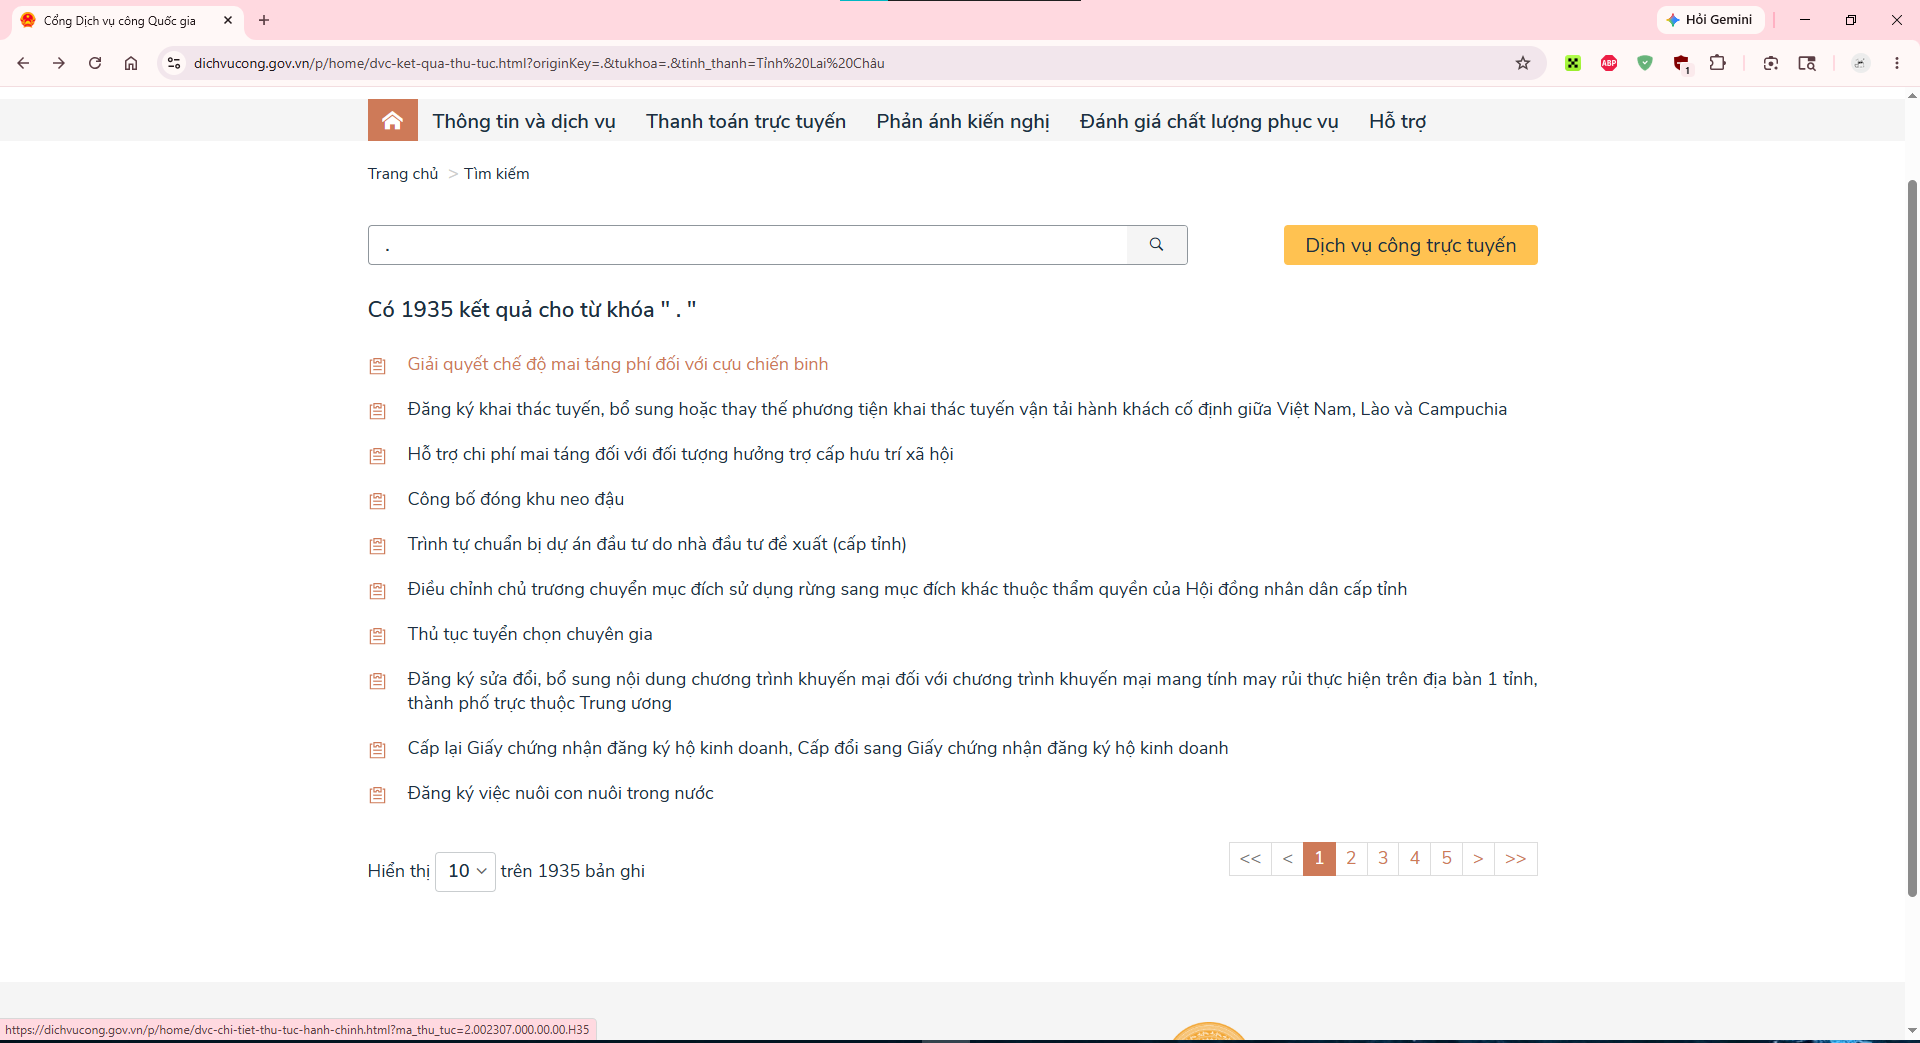
\includegraphics[width=0.92\textwidth]{tai_nguyen/media/image1.png}
\caption{Ảnh màn hình trang tra cứu TTHC trên Cổng Dịch vụ công tỉnh Lai Châu}
\label{fig:2-1}
\end{figure}

\begin{figure}[H]
\centering
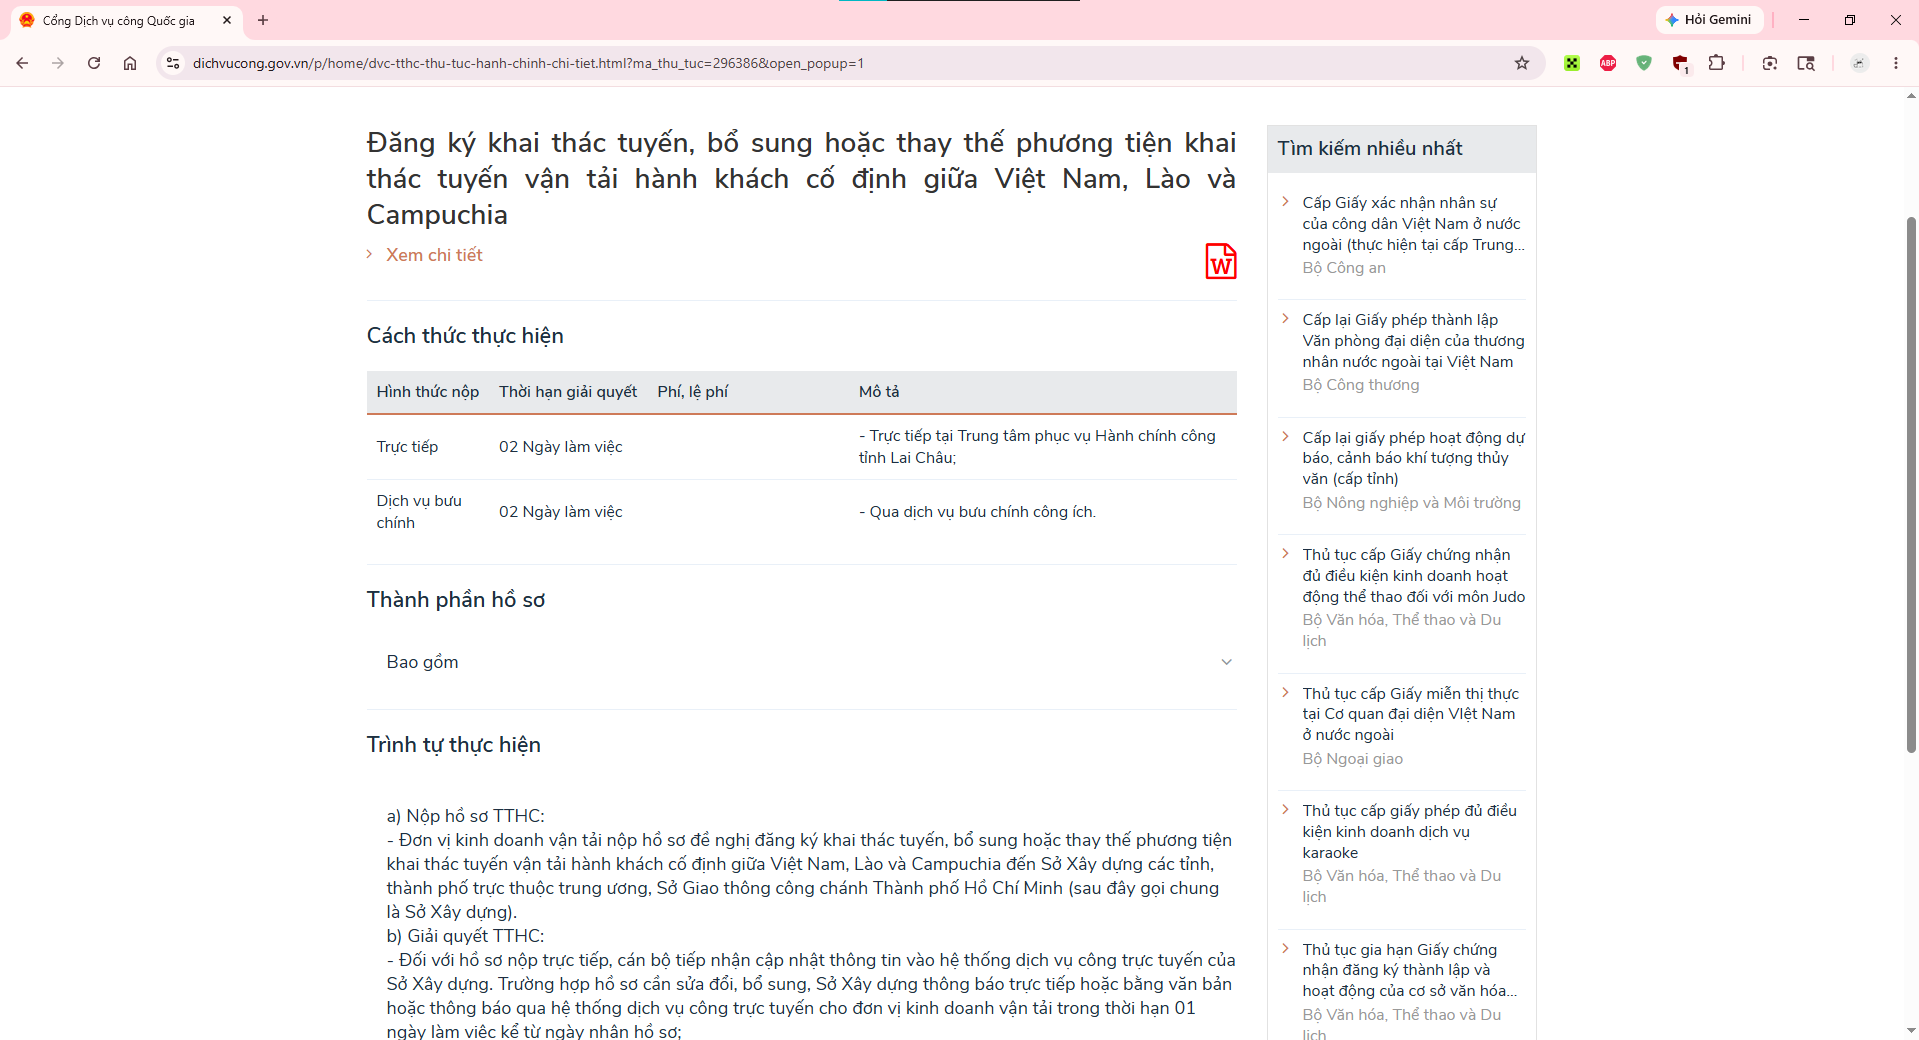
\includegraphics[width=0.92\textwidth]{tai_nguyen/media/image2.png}
\caption{Ảnh màn hình trang chi tiết một TTHC trước khi chuẩn hóa dữ liệu}
\label{fig:2-2}
\end{figure}

\begin{longtable}[]{|
  >{\raggedright\arraybackslash}p{(\columnwidth - 2\tabcolsep) * \real{0.2491}}|
  >{\raggedright\arraybackslash}p{(\columnwidth - 2\tabcolsep) * \real{0.7509}}|}
\caption{Minh chứng nguồn dữ liệu và xử lý dữ liệu đầu vào}\\
\hline
\begin{minipage}[b]{\linewidth}\raggedright
\textbf{Nội dung}
\end{minipage} & \begin{minipage}[b]{\linewidth}\raggedright
\textbf{Mô tả trong đồ án}
\end{minipage} \\
\hline
\endfirsthead
\continuedcaption{Minh chứng nguồn dữ liệu và xử lý dữ liệu đầu vào}
\hline
\begin{minipage}[b]{\linewidth}\raggedright
\textbf{Nội dung}
\end{minipage} & \begin{minipage}[b]{\linewidth}\raggedright
\textbf{Mô tả trong đồ án}
\end{minipage} \\
\hline
\endhead
\hline
\endlastfoot
Nguồn dữ liệu & Cổng Dịch vụ công tỉnh Lai Châu và trang chi tiết thủ
tục hành chính công khai. \\
\hline
Thời điểm chốt dữ liệu & Tháng 10/05/2026, phục vụ phiên bản thử nghiệm
của đồ án. \\
\hline
Định dạng ban đầu & Dữ liệu chi tiết thủ tục dạng văn bản/bảng trên
trang web, sau đó chuẩn hóa sang JSON. \\
\hline
Quy mô dữ liệu & 1950 thủ tục, 176 lĩnh vực, 1950 nhóm thực thể nhận
diện tên thủ tục. \\
\hline
Kiểm tra trùng/lỗi & Không ghi nhận mã thủ tục trùng; loại bỏ giá trị
rỗng/không quy định; chuẩn hóa cách biểu diễn phí, lệ phí và thành phần
hồ sơ. \\
\hline
\end{longtable}

Từ khảo sát thực tế, các khó khăn chính của người dùng nằm ở việc không
biết đúng tên thủ tục, nội dung thủ tục dài, văn phong pháp lý khó đọc
và thông tin cần tìm nằm rải rác. Điều này dẫn tới yêu cầu hệ thống phải
hỗ trợ hỏi bằng ngôn ngữ tự nhiên, truy xuất theo ngữ nghĩa và trình bày
lại câu trả lời ngắn gọn hơn văn bản gốc.

\begin{longtable}[]{|
  >{\raggedright\arraybackslash}p{(\columnwidth - 4\tabcolsep) * \real{0.2497}}|
  >{\raggedright\arraybackslash}p{(\columnwidth - 4\tabcolsep) * \real{0.3409}}|
  >{\raggedright\arraybackslash}p{(\columnwidth - 4\tabcolsep) * \real{0.4094}}|}
\caption{Tổng hợp vấn đề trong quá trình tra cứu TTHC}\\
\hline
\begin{minipage}[b]{\linewidth}\raggedright
\textbf{Nhóm vấn đề}
\end{minipage} & \begin{minipage}[b]{\linewidth}\raggedright
\textbf{Biểu hiện}
\end{minipage} & \begin{minipage}[b]{\linewidth}\raggedright
\textbf{Tác động đến thiết kế hệ thống}
\end{minipage} \\
\hline
\endfirsthead
\continuedcaption{Tổng hợp vấn đề trong quá trình tra cứu TTHC}
\hline
\begin{minipage}[b]{\linewidth}\raggedright
\textbf{Nhóm vấn đề}
\end{minipage} & \begin{minipage}[b]{\linewidth}\raggedright
\textbf{Biểu hiện}
\end{minipage} & \begin{minipage}[b]{\linewidth}\raggedright
\textbf{Tác động đến thiết kế hệ thống}
\end{minipage} \\
\hline
\endhead
\hline
\endlastfoot
Tên thủ tục khó nhớ & Người dân mô tả nhu cầu bằng ngôn ngữ đời thường.
& Cần nhận diện biến thể từ khóa và tìm kiếm theo ngữ nghĩa. \\
\hline
Thông tin nằm rải rác & Hồ sơ, phí, thời hạn, cơ quan tiếp nhận ở các
mục khác nhau. & Cần chunk dữ liệu theo nhóm thông tin. \\
\hline
Văn phong pháp lý & Nhiều đoạn dài, khó đọc với người dùng phổ thông. &
Cần LLM diễn giải lại nhưng phải bám nguồn. \\
\hline
Dữ liệu thay đổi & Thủ tục có thể được cập nhật theo văn bản mới. & Cần
cơ chế cập nhật JSON và build lại VectorDB. \\
\hline
Độ chính xác cao & Trả lời sai có thể làm người dân chuẩn bị sai hồ sơ.
& Prompt phải ràng buộc, không trả lời ngoài context. \\
\hline
\end{longtable}

\section{Phân tích dữ liệu đầu
vào}

Dữ liệu đầu vào chính của hệ thống là file procedures.json, được chuẩn
hóa từ các trang chi tiết TTHC. Mỗi thủ tục gồm mã thủ tục, tên thủ tục
và phần content chứa các trường nghiệp vụ như lĩnh vực, đối tượng thực
hiện, cơ quan thực hiện, cách thức thực hiện, thành phần hồ sơ, thời hạn
giải quyết, phí, lệ phí, kết quả thực hiện và căn cứ pháp lý.

Bộ dữ liệu thử nghiệm được chốt trong tháng 05/2026, gồm 1950 TTHC thuộc
176 lĩnh vực. Trong quá trình làm sạch, các bản ghi được kiểm tra theo
mã thủ tục và tên thủ tục để hạn chế trùng lặp. Các giá trị rỗng, không
quy định hoặc không có thông tin được xử lý riêng để tránh đưa nội dung
nhiễu vào ChromaDB.

\begin{longtable}[]{|
  >{\raggedright\arraybackslash}p{(\columnwidth - 2\tabcolsep) * \real{0.2967}}|
  >{\raggedright\arraybackslash}p{(\columnwidth - 2\tabcolsep) * \real{0.7033}}|}
\caption{Ví dụ thủ tục thật trước và sau khi đưa vào hệ thống}\\
\hline
\begin{minipage}[b]{\linewidth}\raggedright
\textbf{Trạng thái dữ liệu}
\end{minipage} & \begin{minipage}[b]{\linewidth}\raggedright
\textbf{Ví dụ mô tả}
\end{minipage} \\
\hline
\endfirsthead
\continuedcaption{Ví dụ thủ tục thật trước và sau khi đưa vào hệ thống}
\hline
\begin{minipage}[b]{\linewidth}\raggedright
\textbf{Trạng thái dữ liệu}
\end{minipage} & \begin{minipage}[b]{\linewidth}\raggedright
\textbf{Ví dụ mô tả}
\end{minipage} \\
\hline
\endhead
\hline
\endlastfoot
Trên cổng dịch vụ công & Người dùng phải đọc trang chi tiết thủ tục, tự
tìm các mục hồ sơ, thời hạn, cơ quan thực hiện và căn cứ pháp lý. \\
\hline
Trong procedures.json & Thông tin được lưu theo các trường có cấu trúc:
id, name, content, trong đó content chứa Lĩnh vực, Cách thức thực hiện,
Thành phần hồ sơ, Phí, Lệ phí, Căn cứ pháp lý... \\
\hline
Trong ChromaDB & Mỗi nhóm thông tin được chuyển thành chunk riêng, ví dụ
chunk tổng quan, chunk cách thức thực hiện, chunk thành phần hồ sơ và
chunk căn cứ pháp lý. \\
\hline
Khi hỏi chatbot & Câu hỏi ``mai táng phí cựu chiến binh cần hồ sơ gì?''
được ánh xạ tới chunk Thành phần hồ sơ thay vì trả lại toàn bộ thủ
tục. \\
\hline
\end{longtable}

\begin{longtable}[]{|
  >{\raggedright\arraybackslash}p{(\columnwidth - 4\tabcolsep) * \real{0.2181}}|
  >{\raggedright\arraybackslash}p{(\columnwidth - 4\tabcolsep) * \real{0.2336}}|
  >{\raggedright\arraybackslash}p{(\columnwidth - 4\tabcolsep) * \real{0.5483}}|}
\caption{Thống kê dữ liệu đầu vào phục vụ hệ thống RAG}\\
\hline
\begin{minipage}[b]{\linewidth}\raggedright
\textbf{Loại dữ liệu}
\end{minipage} & \begin{minipage}[b]{\linewidth}\raggedright
\textbf{Số lượng/quy mô}
\end{minipage} & \begin{minipage}[b]{\linewidth}\raggedright
\textbf{Vai trò trong hệ thống}
\end{minipage} \\
\hline
\endfirsthead
\continuedcaption{Thống kê dữ liệu đầu vào phục vụ hệ thống RAG}
\hline
\begin{minipage}[b]{\linewidth}\raggedright
\textbf{Loại dữ liệu}
\end{minipage} & \begin{minipage}[b]{\linewidth}\raggedright
\textbf{Số lượng/quy mô}
\end{minipage} & \begin{minipage}[b]{\linewidth}\raggedright
\textbf{Vai trò trong hệ thống}
\end{minipage} \\
\hline
\endhead
\hline
\endlastfoot
Thủ tục hành chính & 1950 thủ tục & Dữ liệu gốc để tra cứu và sinh câu
trả lời. \\
\hline
Lĩnh vực thủ tục & 176 lĩnh vực & Hỗ trợ lọc, nhóm và phân tích dữ liệu
theo nghiệp vụ. \\
\hline
Thực thể tên thủ tục & 1950 nhóm thực thể & Nhận diện tên thủ tục và
biến thể từ khóa trong câu hỏi. \\
\hline
Intent hội thoại & 19 intent & Xử lý chào hỏi, cảm ơn, câu hỏi chung và
ngoài phạm vi. \\
\hline
Nhóm từ đồng nghĩa & 10 nhóm & Chuẩn hóa cách người dùng hỏi về hồ sơ,
phí, thời hạn, cơ quan, pháp lý. \\
\hline
Semantic chunk & Khoảng 30125 chunk & Lưu trong ChromaDB để truy xuất
theo ngữ nghĩa. \\
\hline
\end{longtable}

\emph{Các số liệu trong bảng được tổng hợp từ bộ dữ liệu đã chuẩn hóa
của hệ thống. Chi tiết thống kê dữ liệu thử nghiệm được trình bày tại
Phụ lục C.}

Khi build kho tri thức thử nghiệm, semantic chunker tạo các chunk từ dữ
liệu nguồn. Các chunk được phân nhóm thành tổng quan, cách thức thực
hiện, thành phần hồ sơ, căn cứ pháp lý và các trường đơn giản. Mỗi chunk
gắn metadata để pipeline có thể lọc theo thủ tục, lĩnh vực hoặc field
trước khi đưa vào LLM.

\section{Phân tích bài toán và phạm vi hệ
thống}

Bài toán của đề tài là tạo ra một lớp hỗ trợ tra cứu các TTHC bằng hội
thoại. Hệ thống không thay thế cổng dịch vụ công, không tiếp nhận hồ sơ
chính thức, không xử lý thanh toán và không thay thế thẩm quyền chuyên
môn của cán bộ hành chính. Phạm vi phù hợp của hệ thống là hỗ trợ người
dân tìm đúng thông tin cần biết trước khi chuẩn bị hồ sơ.

Người dùng chính gồm người dân và quản trị viên. Người dân sử dụng
chatbot để hỏi thông tin, tra cứu thủ tục, xem chi tiết thủ tục và xem
lại lịch sử hội thoại. Quản trị viên dùng dashboard để quản lý dữ liệu
thủ tục, theo dõi lịch sử, đồng bộ lại vector database và quản lý quyền
admin. Các dịch vụ như Firebase, Firestore, ChromaDB và LLM là thành
phần hỗ trợ kỹ thuật trong luồng xử lý.

\begin{longtable}[]{|
  >{\raggedright\arraybackslash}p{(\columnwidth - 4\tabcolsep) * \real{0.1249}}|
  >{\raggedright\arraybackslash}p{(\columnwidth - 4\tabcolsep) * \real{0.4381}}|
  >{\raggedright\arraybackslash}p{(\columnwidth - 4\tabcolsep) * \real{0.4370}}|}
\caption{Phạm vi thực hiện của hệ thống}\\
\hline
\begin{minipage}[b]{\linewidth}\raggedright
\textbf{Nội dung}
\end{minipage} & \begin{minipage}[b]{\linewidth}\raggedright
\textbf{Trong phạm vi đồ án}
\end{minipage} & \begin{minipage}[b]{\linewidth}\raggedright
\textbf{Ngoài phạm vi đồ án}
\end{minipage} \\
\hline
\endfirsthead
\continuedcaption{Phạm vi thực hiện của hệ thống}
\hline
\begin{minipage}[b]{\linewidth}\raggedright
\textbf{Nội dung}
\end{minipage} & \begin{minipage}[b]{\linewidth}\raggedright
\textbf{Trong phạm vi đồ án}
\end{minipage} & \begin{minipage}[b]{\linewidth}\raggedright
\textbf{Ngoài phạm vi đồ án}
\end{minipage} \\
\hline
\endhead
\hline
\endlastfoot
Tra cứu thông tin & Hỏi đáp về hồ sơ, thời hạn, phí/lệ phí, cơ quan, kết
quả, căn cứ pháp lý. & Không xác nhận tính hợp lệ cuối cùng của hồ sơ
như cán bộ chuyên môn. \\
\hline
Xem chi tiết thủ tục & Hiển thị/tra cứu thông tin chi tiết của một thủ
tục trong kho dữ liệu đã nạp. & Không thay thế văn bản gốc hoặc quyết
định công bố chính thức. \\
\hline
Tương tác & Hỏi đáp văn bản tiếng Việt qua giao diện web. & Chưa xử lý
giọng nói, ảnh giấy tờ hoặc OCR. \\
\hline
Dữ liệu & Sử dụng procedures.json và các file hỗ trợ entities, synonyms,
intents, codes. & Chưa kết nối trực tiếp toàn bộ hệ thống nghiệp vụ của
cơ quan nhà nước. \\
\hline
Triển khai & Chạy local, hosting frontend, backend thử nghiệm qua
server/ngrok. & Chưa vận hành như dịch vụ công chính thức ở quy mô
tỉnh. \\
\hline
\end{longtable}

\section{Phân tích tác nhân và nhu cầu sử
dụng}

Hai tác nhân trực tiếp là người dùng và quản trị viên. Người dùng quan
tâm đến tra cứu, xem chi tiết thủ tục, hỏi đáp chatbot và xem lại lịch
sử. Quản trị viên quan tâm đến quản lý dữ liệu, đồng bộ VectorDB, giám
sát hệ thống và quản lý quyền. Các thành phần Firebase Authentication,
Firestore, ChromaDB và LLM được xem là hệ thống phụ trợ tham gia vào quá
trình thực hiện nghiệp vụ.

\begin{longtable}[]{|
  >{\raggedright\arraybackslash}p{(\columnwidth - 4\tabcolsep) * \real{0.1797}}|
  >{\raggedright\arraybackslash}p{(\columnwidth - 4\tabcolsep) * \real{0.4507}}|
  >{\raggedright\arraybackslash}p{(\columnwidth - 4\tabcolsep) * \real{0.3695}}|}
\caption{Tác nhân và nhu cầu sử dụng}\\
\hline
\begin{minipage}[b]{\linewidth}\raggedright
\textbf{Tác nhân}
\end{minipage} & \begin{minipage}[b]{\linewidth}\raggedright
\textbf{Use Case chính}
\end{minipage} & \begin{minipage}[b]{\linewidth}\raggedright
\textbf{Vai trò}
\end{minipage} \\
\hline
\endfirsthead
\continuedcaption{Tác nhân và nhu cầu sử dụng}
\hline
\begin{minipage}[b]{\linewidth}\raggedright
\textbf{Tác nhân}
\end{minipage} & \begin{minipage}[b]{\linewidth}\raggedright
\textbf{Use Case chính}
\end{minipage} & \begin{minipage}[b]{\linewidth}\raggedright
\textbf{Vai trò}
\end{minipage} \\
\hline
\endhead
\hline
\endlastfoot
Người dùng & UC01 Đăng nhập; UC02 Tra cứu thủ tục; UC03 Xem chi tiết thủ
tục; UC04 Hỏi đáp chatbot; UC05 Xem lịch sử & Tìm hiểu thông tin thủ tục
và quản lý lịch sử hỏi đáp cá nhân. \\
\hline
Quản trị viên & UC06 Quản lý dữ liệu; UC07 Đồng bộ VectorDB; UC08 Quản
lý admin; UC09 Chuyển văn bản sang JSON; UC10 Giám sát hệ thống & Vận
hành kho dữ liệu và theo dõi hoạt động chatbot. \\
\hline
Firebase Auth & Xác thực token & Cung cấp định danh để backend kiểm tra
quyền truy cập. \\
\hline
Firestore & Lưu sessions, messages, OTP, settings & Lưu dữ liệu nghiệp
vụ và cấu hình. \\
\hline
ChromaDB & Truy xuất vector & Lưu embedding và metadata của các chunk
thủ tục. \\
\hline
LLM & Sinh câu trả lời, hỗ trợ JSON & Diễn giải context RAG và hỗ trợ
admin tạo dữ liệu ban đầu. \\
\hline
\end{longtable}

\section{Phân tích quy trình nghiệp
vụ}

Các quy trình nghiệp vụ được phân tách theo ba nhóm chính: quy trình
người dân tra cứu thủ tục, quy trình hỏi đáp bằng chatbot và quy trình
quản trị dữ liệu TTHC. Cách tách này giúp thể hiện rõ hệ thống không chỉ
là một chatbot trả lời câu hỏi mà còn gồm lớp tra cứu có cấu trúc và lớp
vận hành kho tri thức.

\subsection{Quy trình người dân tra cứu thủ tục hành
chính}
Quy trình tra cứu truyền thống trong phạm vi hệ thống bắt đầu khi người
dân nhập từ khóa hoặc nhu cầu thực tế. Frontend gửi yêu cầu tìm kiếm,
backend chuẩn hóa từ khóa và đối chiếu với dữ liệu thủ tục theo tên,
lĩnh vực hoặc metadata. Kết quả trả về là danh sách thủ tục liên quan để
người dùng mở chi tiết hoặc tiếp tục hỏi chatbot.

\begin{itemize}
\item
  Bước 1: Người dân nhập từ khóa, tên thủ tục hoặc mô tả nhu cầu.
\item
  Bước 2: Hệ thống chuẩn hóa truy vấn và tìm thủ tục liên quan trong kho
  dữ liệu.
\item
  Bước 3: Frontend hiển thị danh sách thủ tục phù hợp.
\item
  Bước 4: Người dân chọn một thủ tục để xem thông tin chi tiết hoặc
  chuyển sang hỏi chatbot.
\end{itemize}

\subsection{Quy trình hỏi đáp thủ tục hành chính bằng
chatbot}
Quy trình hỏi đáp được mô tả theo hướng BPMN. Sơ đồ cần có pool/lane,
start event, end event, task, gateway và data store để thể hiện rõ vai
trò của người dân, frontend, backend, kho tri thức và mô hình AI. Trong
bản Word này, sơ đồ BPMN hiện có được chuyển sang đúng mục 2.5.2 để khớp
với luồng hỏi đáp bằng chatbot.

\begin{figure}[H]
\centering
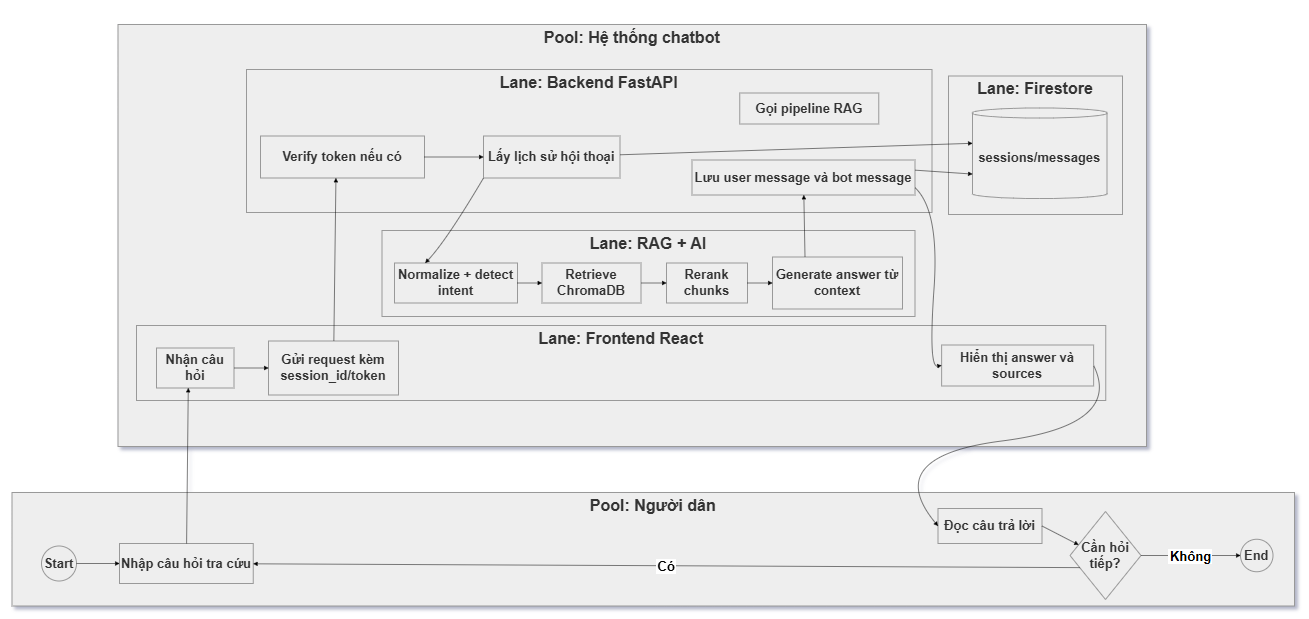
\includegraphics[width=0.92\textwidth]{tai_nguyen/media/image3.png}
\caption{Sơ đồ BPMN quy trình hỏi đáp TTHC bằng chatbot}
\label{fig:2-3}
\end{figure}

Quy trình bắt đầu từ nhu cầu tra cứu của người dân. Sau khi người dân
nhập câu hỏi, frontend gửi request đến backend. Backend kiểm tra xác
thực, lấy lịch sử hội thoại nếu có, gọi pipeline RAG để truy xuất dữ
liệu từ ChromaDB, xếp hạng lại kết quả và đưa context cho LLM sinh câu
trả lời. Sau khi trả kết quả, hệ thống lưu câu hỏi và câu trả lời vào
Firestore.

\subsection{Quy trình quản trị dữ liệu thủ tục hành
chính}
Quy trình quản trị dữ liệu được thực hiện bởi tài khoản có quyền admin.
Quản trị viên có thể thêm, sửa, xóa dữ liệu thủ tục hoặc dùng chức năng
chuyển văn bản thô sang JSON để tạo bản nháp dữ liệu. Sau khi dữ liệu
được kiểm tra, backend lưu thay đổi vào procedures.json và quản trị viên
kích hoạt reload VectorDB để kho tri thức mới có hiệu lực.

\begin{itemize}
\item
  Bước 1: Quản trị viên đăng nhập và được backend kiểm tra quyền admin.
\item
  Bước 2: Quản trị viên thêm, sửa, xóa hoặc chuyển văn bản thủ tục sang
  JSON.
\item
  Bước 3: Dữ liệu được kiểm tra cấu trúc trước khi lưu vào nguồn dữ
  liệu.
\item
  Bước 4: Hệ thống backup ChromaDB cũ, build lại chunk, embedding và
  metadata.
\item
  Bước 5: VectorDB mới được nạp lại để phục vụ truy vấn chatbot.
\end{itemize}

\section{Phân tích yêu cầu hệ
thống}

Yêu cầu hệ thống được xác định từ hai nhóm nhu cầu: người dân cần tra
cứu nhanh và dễ hiểu, còn quản trị viên cần vận hành dữ liệu an toàn.
Trong hệ thống RAG, yêu cầu không chỉ dừng ở chức năng phần mềm mà còn
phải có tiêu chí đánh giá chất lượng truy xuất và chất lượng câu trả
lời.

\subsection{Yêu cầu chức
năng}
Yêu cầu chức năng được xây dựng từ nhu cầu tra cứu của người dân và nhu
cầu vận hành của quản trị viên. Chức năng ``xem chi tiết thông tin thủ
tục'' được tách riêng, không chỉ xem như kết quả phụ của chatbot. Nhờ
vậy hệ thống có thể phục vụ cả kiểu sử dụng tra cứu có cấu trúc và kiểu
hỏi đáp tự nhiên.

\begin{longtable}[]{|
  >{\raggedright\arraybackslash}p{(\columnwidth - 4\tabcolsep) * \real{0.0815}}|
  >{\raggedright\arraybackslash}p{(\columnwidth - 4\tabcolsep) * \real{0.2665}}|
  >{\raggedright\arraybackslash}p{(\columnwidth - 4\tabcolsep) * \real{0.6520}}|}
\caption{Yêu cầu chức năng của hệ thống}\\
\hline
\begin{minipage}[b]{\linewidth}\raggedright
\textbf{Mã}
\end{minipage} & \begin{minipage}[b]{\linewidth}\raggedright
\textbf{Tên yêu cầu}
\end{minipage} & \begin{minipage}[b]{\linewidth}\raggedright
\textbf{Mô tả ngắn gọn}
\end{minipage} \\
\hline
\endfirsthead
\continuedcaption{Yêu cầu chức năng của hệ thống}
\hline
\begin{minipage}[b]{\linewidth}\raggedright
\textbf{Mã}
\end{minipage} & \begin{minipage}[b]{\linewidth}\raggedright
\textbf{Tên yêu cầu}
\end{minipage} & \begin{minipage}[b]{\linewidth}\raggedright
\textbf{Mô tả ngắn gọn}
\end{minipage} \\
\hline
\endhead
\hline
\endlastfoot
FR01 & Đăng nhập và xác thực & Người dùng đăng nhập bằng email/Google;
backend xác minh token bằng Firebase Admin SDK. \\
\hline
FR02 & Tra cứu thủ tục theo ngữ nghĩa & Người dùng nhập từ khóa hoặc nhu
cầu đời thường để tìm thủ tục liên quan. \\
\hline
FR03 & Xem chi tiết thông tin thủ tục & Người dùng xem các mục chi tiết
của một thủ tục: hồ sơ, cơ quan, thời hạn, phí, kết quả, căn cứ pháp
lý. \\
\hline
FR04 & Hỏi đáp chatbot RAG & Người dùng đặt câu hỏi tự nhiên và nhận câu
trả lời dựa trên context đã truy xuất. \\
\hline
FR05 & Lưu và xem lịch sử hội thoại & Câu hỏi và câu trả lời được lưu
theo session trong Firestore. \\
\hline
FR06 & Quản lý dữ liệu thủ tục & Admin thêm, sửa, xóa và xem danh sách
thủ tục trong procedures.json. \\
\hline
FR07 & Đồng bộ VectorDB & Admin build lại ChromaDB sau khi dữ liệu thủ
tục thay đổi, có backup trước khi build. \\
\hline
FR08 & Quản lý quyền admin & Super admin cấp hoặc thu hồi quyền quản trị
theo email. \\
\hline
FR09 & Thống kê và giám sát & Admin xem số user, số phiên, biểu đồ 7
ngày và lịch sử hội thoại. \\
\hline
FR10 & Chuyển văn bản sang JSON & Admin dán văn bản thủ tục thô, hệ
thống dùng AI tạo bản nháp JSON. \\
\hline
\end{longtable}

\subsection{Yêu cầu phi chức năng và tiêu chí chấp
nhận}
Yêu cầu phi chức năng trong hệ thống RAG cần có tiêu chí chấp nhận cụ
thể để phục vụ kiểm thử. Các ngưỡng dưới đây được đặt cho phạm vi đồ án
và môi trường thử nghiệm, không phải cam kết vận hành chính thức. Khi
triển khai quy mô lớn, các ngưỡng này cần được đo lại trên hạ tầng thật
và bộ câu hỏi có đáp án chuẩn.

\begin{longtable}[]{|
  >{\raggedright\arraybackslash}p{(\columnwidth - 4\tabcolsep) * \real{0.2028}}|
  >{\raggedright\arraybackslash}p{(\columnwidth - 4\tabcolsep) * \real{0.4521}}|
  >{\raggedright\arraybackslash}p{(\columnwidth - 4\tabcolsep) * \real{0.3451}}|}
\caption{Yêu cầu phi chức năng và tiêu chí chấp nhận}\\
\hline
\begin{minipage}[b]{\linewidth}\raggedright
\textbf{Nhóm yêu cầu}
\end{minipage} & \begin{minipage}[b]{\linewidth}\raggedright
\textbf{Tiêu chí chấp nhận trong đồ án}
\end{minipage} & \begin{minipage}[b]{\linewidth}\raggedright
\textbf{Cách kiểm tra}
\end{minipage} \\
\hline
\endfirsthead
\continuedcaption{Yêu cầu phi chức năng và tiêu chí chấp nhận}
\hline
\begin{minipage}[b]{\linewidth}\raggedright
\textbf{Nhóm yêu cầu}
\end{minipage} & \begin{minipage}[b]{\linewidth}\raggedright
\textbf{Tiêu chí chấp nhận trong đồ án}
\end{minipage} & \begin{minipage}[b]{\linewidth}\raggedright
\textbf{Cách kiểm tra}
\end{minipage} \\
\hline
\endhead
\hline
\endlastfoot
Độ chính xác truy xuất & Top-5 context chứa đúng thủ tục hoặc đúng
trường thông tin đạt tối thiểu 85\% trên bộ câu hỏi thử nghiệm. & Kiểm
tra thủ công context được truy xuất theo từng câu hỏi mẫu. \\
\hline
Độ đúng câu trả lời & Tỉ lệ câu trả lời đúng theo dữ liệu nguồn đạt tối
thiểu 80\% trên bộ câu hỏi có đáp án đối chiếu. & So sánh câu trả lời
với procedures.json và trang nguồn. \\
\hline
Từ chối khi thiếu dữ liệu & Tối thiểu 90\% câu hỏi ngoài phạm vi phải
trả lời theo hướng ``Dữ liệu hiện tại không đề cập''. & Kiểm thử nhóm
câu hỏi gây nhiễu/ngoài phạm vi. \\
\hline
Thời gian phản hồi & Câu xã giao dưới 1 giây; câu hỏi RAG thông thường
trung bình dưới 8 giây trong môi trường thử nghiệm. & Ghi log thời gian
từ lúc gửi request đến lúc nhận answer. \\
\hline
Người dùng đồng thời & Phục vụ thử nghiệm 5-10 người dùng đồng thời với
các truy vấn ngắn, không treo giao diện. & Kiểm thử tải nhẹ bằng nhiều
phiên trình duyệt hoặc công cụ gửi request. \\
\hline
Bảo mật & Endpoint admin trả 403 với tài khoản thường; endpoint cần đăng
nhập trả 401 khi không có token. & Gọi API bằng tài khoản thường và
request không có Authorization. \\
\hline
Khả năng mở rộng dữ liệu & Có thể thêm/sửa thủ tục và reload VectorDB mà
không sửa mã nguồn pipeline. & Cập nhật procedures.json qua dashboard
rồi build lại ChromaDB. \\
\hline
\end{longtable}

\section{Sơ đồ Use Case và đặc tả Use Case
chính}

Use Case được dùng để mô tả hệ thống từ góc nhìn tác nhân sử dụng. Trong
chương này, sơ đồ Use Case tổng quát cho biết toàn bộ chức năng chính
của hệ thống, còn sơ đồ phân rã Use Case tách riêng nhóm chức năng của
người dùng và nhóm chức năng của quản trị viên.

\subsection{Sơ đồ Use Case tổng
quát}
\begin{figure}[H]
\centering
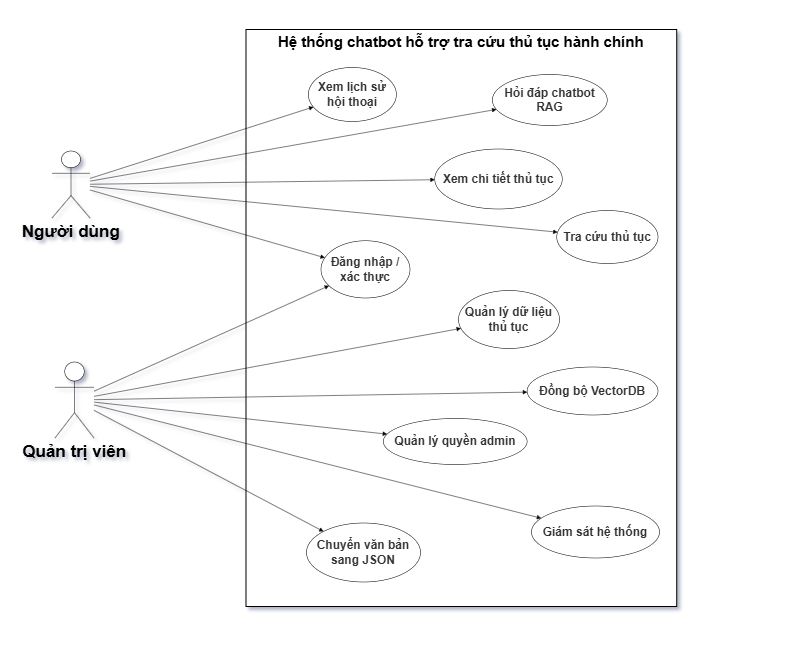
\includegraphics[width=0.92\textwidth]{tai_nguyen/media/image4.png}
\caption{Sơ đồ Use Case tổng quát của hệ thống}
\label{fig:2-4}
\end{figure}

Sơ đồ Use Case tổng quát thể hiện hai tác nhân chính và các chức năng
bắt buộc: tra cứu thủ tục, xem chi tiết thông tin thủ tục, hỏi đáp bằng
chatbot, lưu/xem lịch sử, quản lý dữ liệu thủ tục và quản lý hoạt động
hệ thống. Use Case ``Xem chi tiết thông tin thủ tục'' được tách riêng vì
đây là chức năng độc lập với luồng hỏi đáp chatbot.

\subsection{Sơ đồ Use Case nhóm người
dùng}
\begin{figure}[H]
\centering
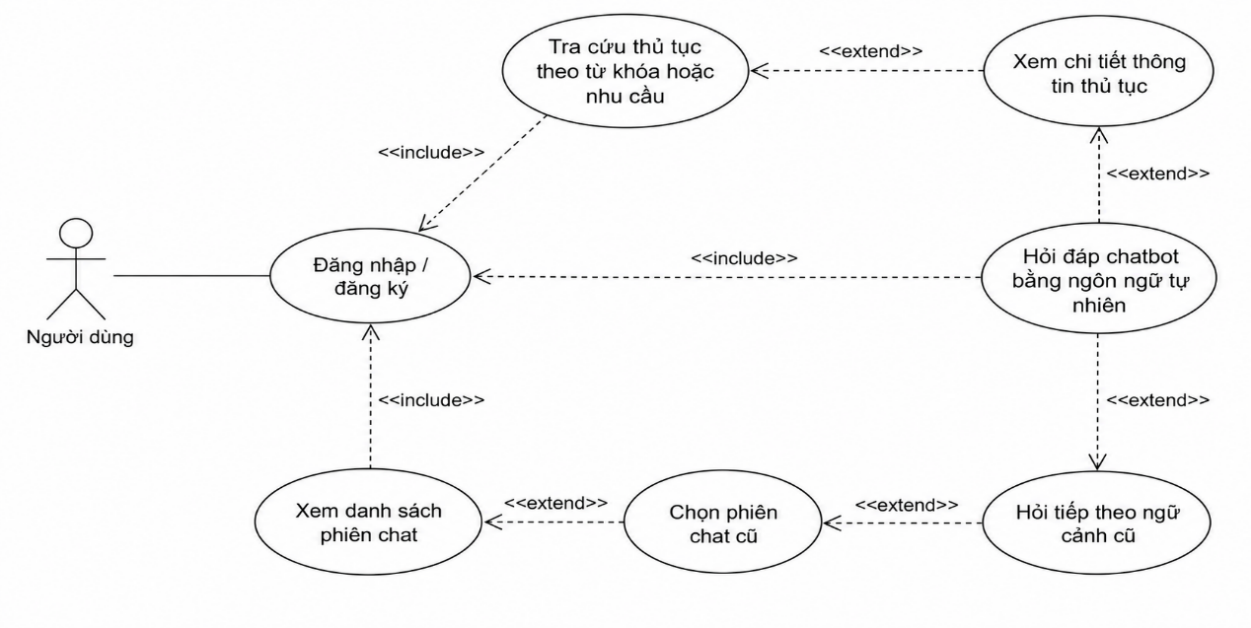
\includegraphics[width=0.92\textwidth]{tai_nguyen/media/image5.png}
\caption{Sơ đồ Use Case nhóm người dùng}
\label{fig:2-5}
\end{figure}

Nhóm Use Case của người dùng thể hiện rõ đường đi từ tra cứu đến xem chi
tiết và hỏi đáp. Người dùng có thể tìm thủ tục theo nhu cầu, mở thông
tin chi tiết, hỏi tiếp các trường cụ thể hoặc quay lại lịch sử hội thoại
đã lưu.

\subsection{Sơ đồ Use Case nhóm quản trị
viên}
\begin{figure}[H]
\centering
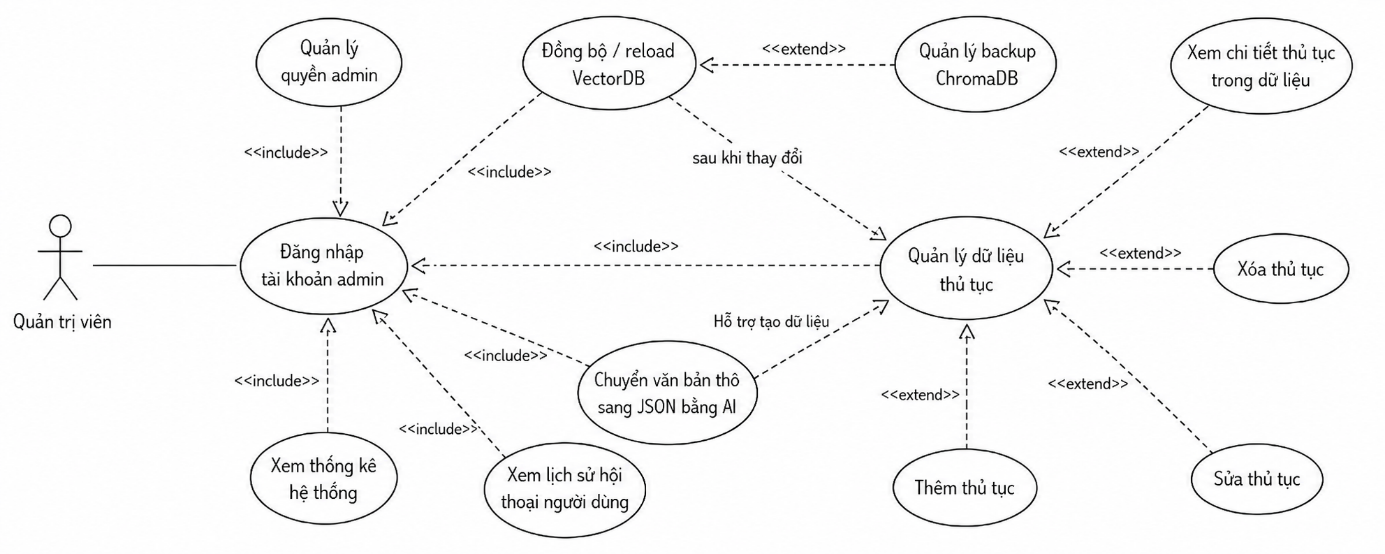
\includegraphics[width=0.92\textwidth]{tai_nguyen/media/image6.png}
\caption{Sơ đồ Use Case nhóm quản trị viên}
\label{fig:2-6}
\end{figure}

Nhóm Use Case của quản trị viên tập trung vào vận hành dữ liệu. Các chức
năng thêm/sửa/xóa thủ tục, chuyển văn bản sang JSON, đồng bộ VectorDB và
quản lý backup có tác động trực tiếp đến chất lượng kho tri thức, vì vậy
phải được bảo vệ bằng quyền admin ở backend.

\subsection{Đặc tả các Use Case
chính}

\begin{longtable}[]{|
  >{\raggedright\arraybackslash}p{(\columnwidth - 4\tabcolsep) * \real{0.1500}}|
  >{\raggedright\arraybackslash}p{(\columnwidth - 4\tabcolsep) * \real{0.4752}}|
  >{\raggedright\arraybackslash}p{(\columnwidth - 4\tabcolsep) * \real{0.3749}}|}
\caption{Tác nhân và Use Case chính}\\
\hline
\begin{minipage}[b]{\linewidth}\raggedright
\textbf{Tác nhân}
\end{minipage} & \begin{minipage}[b]{\linewidth}\raggedright
\textbf{Use Case chính}
\end{minipage} & \begin{minipage}[b]{\linewidth}\raggedright
\textbf{Vai trò}
\end{minipage} \\
\hline
\endfirsthead
\continuedcaption{Tác nhân và Use Case chính}
\hline
\begin{minipage}[b]{\linewidth}\raggedright
\textbf{Tác nhân}
\end{minipage} & \begin{minipage}[b]{\linewidth}\raggedright
\textbf{Use Case chính}
\end{minipage} & \begin{minipage}[b]{\linewidth}\raggedright
\textbf{Vai trò}
\end{minipage} \\
\hline
\endhead
\hline
\endlastfoot
Người dùng & UC01 Đăng nhập; UC02 Tra cứu thủ tục; UC03 Xem chi tiết thủ
tục; UC04 Hỏi đáp chatbot; UC05 Xem lịch sử & Tìm hiểu thông tin thủ tục
và quản lý lịch sử hỏi đáp cá nhân. \\
\hline
Quản trị viên & UC06 Quản lý dữ liệu; UC07 Đồng bộ VectorDB; UC08 Quản
lý admin; UC09 Chuyển văn bản sang JSON; UC10 Giám sát hệ thống & Vận
hành kho dữ liệu và theo dõi hoạt động chatbot. \\
\hline
Firebase Auth & Xác thực token & Cung cấp định danh để backend kiểm tra
quyền truy cập. \\
\hline
Firestore & Lưu sessions, messages, OTP, settings & Lưu dữ liệu nghiệp
vụ và cấu hình. \\
\hline
ChromaDB & Truy xuất vector & Lưu embedding và metadata của các chunk
thủ tục. \\
\hline
LLM & Sinh câu trả lời, hỗ trợ JSON & Diễn giải context RAG và hỗ trợ
admin tạo dữ liệu ban đầu. \\
\hline
\end{longtable}

\begin{longtable}[]{|
  >{\raggedright\arraybackslash}p{(\columnwidth - 2\tabcolsep) * \real{0.1559}}|
  >{\raggedright\arraybackslash}p{(\columnwidth - 2\tabcolsep) * \real{0.8441}}|}
\caption{Đặc tả UC01 - Đăng nhập và xác thực người dùng}\\
\hline
\begin{minipage}[b]{\linewidth}\raggedright
\textbf{Mục}
\end{minipage} & \begin{minipage}[b]{\linewidth}\raggedright
\textbf{Nội dung}
\end{minipage} \\
\hline
\endfirsthead
\continuedcaption{Đặc tả UC01 - Đăng nhập và xác thực người dùng}
\hline
\begin{minipage}[b]{\linewidth}\raggedright
\textbf{Mục}
\end{minipage} & \begin{minipage}[b]{\linewidth}\raggedright
\textbf{Nội dung}
\end{minipage} \\
\hline
\endhead
\hline
\endlastfoot
Tác nhân chính & Người dùng, Firebase Authentication, Backend
FastAPI. \\
\hline
Mục tiêu & Người dùng truy cập hệ thống bằng tài khoản hợp lệ và có
token để gọi API cần bảo vệ. \\
\hline
Tiền điều kiện & Người dùng có tài khoản Google/email; backend đã cấu
hình Firebase Admin SDK. \\
\hline
Luồng chính & \begin{minipage}[t]{\linewidth}\raggedright
1. Người dùng chọn phương thức đăng nhập.\\
2. Firebase xác thực tài khoản.\\
3. Frontend nhận ID Token.\\
4. Frontend gửi Bearer Token khi gọi API.\\
5. Backend xác minh token và cho phép truy cập.\strut
\end{minipage} \\
\hline
Ngoại lệ & 3.1Token hết hạn, sai định dạng hoặc tài khoản không tồn tại
thì backend từ chối request. \\
\hline
Hậu điều kiện & Người dùng vào giao diện chatbot và có thể lưu lịch sử
hội thoại. \\
\hline
\end{longtable}

\begin{longtable}[]{|
  >{\raggedright\arraybackslash}p{(\columnwidth - 2\tabcolsep) * \real{0.1403}}|
  >{\raggedright\arraybackslash}p{(\columnwidth - 2\tabcolsep) * \real{0.8597}}|}
\caption{Đặc tả UC02 - Tra cứu TTHC}\\
\hline
\begin{minipage}[b]{\linewidth}\raggedright
\textbf{Mục}
\end{minipage} & \begin{minipage}[b]{\linewidth}\raggedright
\textbf{Nội dung}
\end{minipage} \\
\hline
\endfirsthead
\continuedcaption{Đặc tả UC02 - Tra cứu TTHC}
\hline
\begin{minipage}[b]{\linewidth}\raggedright
\textbf{Mục}
\end{minipage} & \begin{minipage}[b]{\linewidth}\raggedright
\textbf{Nội dung}
\end{minipage} \\
\hline
\endhead
\hline
\endlastfoot
Tác nhân chính & Người dùng, Backend, dữ liệu
procedures.json/ChromaDB. \\
\hline
Mục tiêu & Người dùng tìm thủ tục liên quan khi chỉ biết từ khóa hoặc
nhu cầu thực tế. \\
\hline
Tiền điều kiện & Kho dữ liệu thủ tục đã được nạp; frontend kết nối được
backend. \\
\hline
Luồng chính & \begin{minipage}[t]{\linewidth}\raggedright
1. Người dùng nhập từ khóa hoặc nhu cầu.\\
2. Hệ thống chuẩn hóa truy vấn.\\
3. Backend tìm thủ tục liên quan theo tên, biến thể từ khóa hoặc ngữ
nghĩa.\\
4. Frontend hiển thị danh sách hoặc thủ tục phù hợp nhất.\strut
\end{minipage} \\
\hline
Ngoại lệ & 3.1 Không tìm thấy thủ tục phù hợp thì hệ thống gợi ý người
dùng nhập rõ hơn. \\
\hline
Hậu điều kiện & Người dùng có thể chọn thủ tục để xem chi tiết hoặc hỏi
chatbot. \\
\hline
\end{longtable}

\begin{longtable}[]{|
  >{\raggedright\arraybackslash}p{(\columnwidth - 2\tabcolsep) * \real{0.1714}}|
  >{\raggedright\arraybackslash}p{(\columnwidth - 2\tabcolsep) * \real{0.8286}}|}
\caption{Đặc tả UC03 - Xem chi tiết thông tin thủ tục}\\
\hline
\begin{minipage}[b]{\linewidth}\raggedright
\textbf{Mục}
\end{minipage} & \begin{minipage}[b]{\linewidth}\raggedright
\textbf{Nội dung}
\end{minipage} \\
\hline
\endfirsthead
\continuedcaption{Đặc tả UC03 - Xem chi tiết thông tin thủ tục}
\hline
\begin{minipage}[b]{\linewidth}\raggedright
\textbf{Mục}
\end{minipage} & \begin{minipage}[b]{\linewidth}\raggedright
\textbf{Nội dung}
\end{minipage} \\
\hline
\endhead
\hline
\endlastfoot
Tác nhân chính & Người dùng, Frontend, Backend, procedures.json. \\
\hline
Mục tiêu & Hiển thị thông tin chi tiết của một thủ tục độc lập với luồng
hỏi đáp chatbot. \\
\hline
Tiền điều kiện & Thủ tục tồn tại trong dữ liệu nguồn hoặc được tìm thấy
qua tra cứu. \\
\hline
Luồng chính & \begin{minipage}[t]{\linewidth}\raggedright
1. Người dùng chọn một thủ tục.\\
2. Frontend yêu cầu thông tin chi tiết.\\
3. Backend trả các trường hồ sơ, cơ quan, thời hạn, phí/lệ phí, kết quả,
căn cứ pháp lý.\\
4. Frontend hiển thị theo từng nhóm thông tin.\strut
\end{minipage} \\
\hline
Ngoại lệ & 3.1 Nếu thủ tục không tồn tại, hệ thống thông báo không tìm
thấy dữ liệu. \\
\hline
Hậu điều kiện & Người dùng xem được thông tin đầy đủ và có thể tiếp tục
đặt câu hỏi về thủ tục đó. \\
\hline
\end{longtable}

\begin{longtable}[]{|
  >{\raggedright\arraybackslash}p{(\columnwidth - 2\tabcolsep) * \real{0.1715}}|
  >{\raggedright\arraybackslash}p{(\columnwidth - 2\tabcolsep) * \real{0.8285}}|}
\caption{Đặc tả UC04 - Hỏi đáp TTHC bằng chatbot}\\
\hline
\begin{minipage}[b]{\linewidth}\raggedright
\textbf{Mục}
\end{minipage} & \begin{minipage}[b]{\linewidth}\raggedright
\textbf{Nội dung}
\end{minipage} \\
\hline
\endfirsthead
\continuedcaption{Đặc tả UC04 - Hỏi đáp TTHC bằng chatbot}
\hline
\begin{minipage}[b]{\linewidth}\raggedright
\textbf{Mục}
\end{minipage} & \begin{minipage}[b]{\linewidth}\raggedright
\textbf{Nội dung}
\end{minipage} \\
\hline
\endhead
\hline
\endlastfoot
Tác nhân chính & Người dùng, Backend, ChromaDB, Reranker, LLM. \\
\hline
Mục tiêu & Người dùng đặt câu hỏi tự nhiên và nhận câu trả lời dựa trên
dữ liệu đã truy xuất. \\
\hline
Tiền điều kiện & Backend đã khởi động; vector database đã được load hoặc
build thành công. \\
\hline
Luồng chính & \begin{minipage}[t]{\linewidth}\raggedright
1. Người dùng nhập câu hỏi.\\
2. Frontend gửi request đến /user/chat.\\
3. Backend lấy lịch sử session.\\
4. Pipeline RAG truy xuất và rerank dữ liệu.\\
5. LLM sinh câu trả lời từ context.\\
6. Hệ thống trả kết quả và lưu lịch sử.\strut
\end{minipage} \\
\hline
Ngoại lệ & \begin{minipage}[t]{\linewidth}\raggedright
4.1 DB chưa sẵn sàng thì báo đang khởi tạo;\\
6.1 Không có dữ liệu phù hợp thì trả ``Dữ liệu hiện tại không đề
cập''.\strut
\end{minipage} \\
\hline
Hậu điều kiện & Câu hỏi và câu trả lời được lưu vào Firestore theo
session. \\
\hline
\end{longtable}

\begin{longtable}[]{|
  >{\raggedright\arraybackslash}p{(\columnwidth - 2\tabcolsep) * \real{0.1714}}|
  >{\raggedright\arraybackslash}p{(\columnwidth - 2\tabcolsep) * \real{0.8286}}|}
\caption{Đặc tả UC05 - Xem lịch sử hội thoại}\\
\hline
\begin{minipage}[b]{\linewidth}\raggedright
\textbf{Mục}
\end{minipage} & \begin{minipage}[b]{\linewidth}\raggedright
\textbf{Nội dung}
\end{minipage} \\
\hline
\endfirsthead
\continuedcaption{Đặc tả UC05 - Xem lịch sử hội thoại}
\hline
\begin{minipage}[b]{\linewidth}\raggedright
\textbf{Mục}
\end{minipage} & \begin{minipage}[b]{\linewidth}\raggedright
\textbf{Nội dung}
\end{minipage} \\
\hline
\endhead
\hline
\endlastfoot
Tác nhân chính & Người dùng, Frontend, Backend, Firestore. \\
\hline
Mục tiêu & Người dùng mở lại phiên chat đã lưu và tiếp tục hội thoại. \\
\hline
Tiền điều kiện & Người dùng đã đăng nhập và có session đã được tạo. \\
\hline
Luồng chính & \begin{minipage}[t]{\linewidth}\raggedright
1. Frontend gọi /user/sessions.\\
2. Backend truy vấn sessions theo uid.\\
3. Người dùng chọn session.\\
4. Frontend gọi /user/chat/history.\\
5. Tin nhắn được hiển thị theo thứ tự thời gian.\strut
\end{minipage} \\
\hline
Ngoại lệ & \begin{minipage}[t]{\linewidth}\raggedright
2.1 Không có session thì sidebar trống;\\
4.1 Lỗi Firestore thì hệ thống trả danh sách rỗng.\strut
\end{minipage} \\
\hline
Hậu điều kiện & Người dùng có thể tiếp tục hỏi trong session hiện
tại. \\
\hline
\end{longtable}

\begin{longtable}[]{|
  >{\raggedright\arraybackslash}p{(\columnwidth - 2\tabcolsep) * \real{0.1714}}|
  >{\raggedright\arraybackslash}p{(\columnwidth - 2\tabcolsep) * \real{0.8286}}|}
\caption{Đặc tả UC06 - Quản lý dữ liệu TTHC}\\
\hline
\begin{minipage}[b]{\linewidth}\raggedright
\textbf{Mục}
\end{minipage} & \begin{minipage}[b]{\linewidth}\raggedright
\textbf{Nội dung}
\end{minipage} \\
\hline
\endfirsthead
\continuedcaption{Đặc tả UC06 - Quản lý dữ liệu TTHC}
\hline
\begin{minipage}[b]{\linewidth}\raggedright
\textbf{Mục}
\end{minipage} & \begin{minipage}[b]{\linewidth}\raggedright
\textbf{Nội dung}
\end{minipage} \\
\hline
\endhead
\hline
\endlastfoot
Tác nhân chính & Quản trị viên, Backend FastAPI, procedures.json,
Firestore \\
\hline
Mục tiêu & Quản trị viên quản lý danh sách thủ tục hành chính trong hệ
thống, bao gồm thêm, sửa, xóa và kiểm tra dữ liệu trước khi đồng bộ kho
tri thức. \\
\hline
Tiền điều kiện & Tài khoản đã được cấp quyền admin; backend kết nối được
dữ liệu nguồn. \\
\hline
Luồng chính & 1. Quản trị viên truy cập giao diện quản lý dữ liệu.

2. Frontend gửi request lấy danh sách thủ tục.

3. Backend đọc dữ liệu từ procedures.json hoặc collection liên quan.

4. Quản trị viên thực hiện thêm, sửa hoặc xóa thủ tục.

5. Backend kiểm tra dữ liệu đầu vào.

6. Hệ thống lưu dữ liệu mới và cập nhật metadata cần thiết. \\
\hline
Ngoại lệ & \begin{minipage}[t]{\linewidth}\raggedright
5.a Dữ liệu thiếu trường bắt buộc hoặc sai cấu trúc thì hệ thống từ chối
lưu.\\
6.a File dữ liệu đang bị khóa hoặc lỗi ghi thì backend trả thông báo
thất bại.\strut
\end{minipage} \\
\hline
Hậu điều kiện & Dữ liệu thủ tục được cập nhật và sẵn sàng cho quá trình
build lại VectorDB. \\
\hline
\end{longtable}

\begin{longtable}[]{|
  >{\raggedright\arraybackslash}p{(\columnwidth - 2\tabcolsep) * \real{0.1714}}|
  >{\raggedright\arraybackslash}p{(\columnwidth - 2\tabcolsep) * \real{0.8286}}|}
\caption{Đặc tả UC07 - Đồng bộ và xây dựng lại VectorDB}\\
\hline
\begin{minipage}[b]{\linewidth}\raggedright
\textbf{Mục}
\end{minipage} & \begin{minipage}[b]{\linewidth}\raggedright
\textbf{Nội dung}
\end{minipage} \\
\hline
\endfirsthead
\continuedcaption{Đặc tả UC07 - Đồng bộ và xây dựng lại VectorDB}
\hline
\begin{minipage}[b]{\linewidth}\raggedright
\textbf{Mục}
\end{minipage} & \begin{minipage}[b]{\linewidth}\raggedright
\textbf{Nội dung}
\end{minipage} \\
\hline
\endhead
\hline
\endlastfoot
Tác nhân chính & Quản trị viên, Backend FastAPI, ChromaDB, Embedding
Model \\
\hline
Mục tiêu & Đồng bộ lại kho vector sau khi dữ liệu thủ tục thay đổi nhằm
đảm bảo chatbot truy xuất đúng dữ liệu mới nhất. \\
\hline
Tiền điều kiện & Dữ liệu procedures.json hợp lệ; embedding model và
ChromaDB đã được khởi tạo. \\
\hline
Luồng chính & 1. Quản trị viên chọn chức năng đồng bộ VectorDB.

2. Backend kiểm tra dữ liệu JSON đầu vào.

3. Hệ thống backup thư mục ChromaDB hiện tại.

4. Backend thực hiện chunking dữ liệu thủ tục.

5. Embedding model sinh vector cho từng chunk.

6. Hệ thống nạp vector và metadata vào ChromaDB mới.

7. Backend lưu database mới xuống bộ nhớ.

8. Hệ thống trả trạng thái build thành công. \\
\hline
Ngoại lệ & 2.a JSON không hợp lệ thì dừng quá trình đồng bộ.

5.a Embedding model lỗi hoặc hết tài nguyên RAM thì quá trình build bị
hủy.

6.a Không ghi được dữ liệu xuống ChromaDB thì rollback về bản backup
trước đó. \\
\hline
Hậu điều kiện & Kho vector mới được kích hoạt và chatbot sử dụng dữ liệu
đã cập nhật cho các truy vấn tiếp theo. \\
\hline
\end{longtable}

Các Use Case quản trị gồm quản lý dữ liệu thủ tục, đồng bộ VectorDB,
quản lý quyền admin, chuyển văn bản sang JSON và giám sát hệ thống. Các
Use Case này được bảo vệ bằng quyền admin ở backend vì có thể tác động
trực tiếp đến dữ liệu nguồn, lịch sử hội thoại hoặc kho vector của hệ
thống.

\section{Tổng hợp phân tích và lựa chọn giải
pháp
RAG}

Từ các phần khảo sát, phân tích dữ liệu, phạm vi hệ thống, tác nhân, quy
trình nghiệp vụ và yêu cầu hệ thống, có thể thấy bài toán tra cứu TTHC
cần một giải pháp vừa hiểu được ngôn ngữ tự nhiên vừa bám dữ liệu nguồn.
Nếu chỉ dùng tìm kiếm từ khóa, hệ thống khó xử lý các câu hỏi đời thường
hoặc câu hỏi không nêu đúng tên thủ tục. Nếu chỉ dùng LLM thuần túy, câu
trả lời có thể trôi khỏi dữ liệu hành chính công và khó kiểm chứng.

So với chatbot rule-based, RAG linh hoạt hơn khi người dân diễn đạt khác
mẫu câu. So với LLM thuần túy, RAG an toàn hơn vì câu trả lời bị ràng
buộc bởi dữ liệu nguồn. Vì vậy, RAG là phương án phù hợp nhất với mục
tiêu của đề tài: hỗ trợ tra cứu bằng ngôn ngữ tự nhiên nhưng vẫn giữ
được căn cứ dữ liệu hành chính công.

\begin{longtable}[]{|
  >{\raggedright\arraybackslash}p{(\columnwidth - 6\tabcolsep) * \real{0.1582}}|
  >{\raggedright\arraybackslash}p{(\columnwidth - 6\tabcolsep) * \real{0.2424}}|
  >{\raggedright\arraybackslash}p{(\columnwidth - 6\tabcolsep) * \real{0.2401}}|
  >{\raggedright\arraybackslash}p{(\columnwidth - 6\tabcolsep) * \real{0.3592}}|}
\caption{So sánh các giải pháp chatbot cho bài toán tra cứu TTHC}\\
\hline
\begin{minipage}[b]{\linewidth}\raggedright
\textbf{Tiêu chí}
\end{minipage} & \begin{minipage}[b]{\linewidth}\raggedright
\textbf{Rule-based chatbot}
\end{minipage} & \begin{minipage}[b]{\linewidth}\raggedright
\textbf{LLM thuần túy}
\end{minipage} & \begin{minipage}[b]{\linewidth}\raggedright
\textbf{Chatbot RAG đề xuất}
\end{minipage} \\
\hline
\endfirsthead
\continuedcaption{So sánh các giải pháp chatbot cho bài toán tra cứu TTHC}
\hline
\begin{minipage}[b]{\linewidth}\raggedright
\textbf{Tiêu chí}
\end{minipage} & \begin{minipage}[b]{\linewidth}\raggedright
\textbf{Rule-based chatbot}
\end{minipage} & \begin{minipage}[b]{\linewidth}\raggedright
\textbf{LLM thuần túy}
\end{minipage} & \begin{minipage}[b]{\linewidth}\raggedright
\textbf{Chatbot RAG đề xuất}
\end{minipage} \\
\hline
\endhead
\hline
\endlastfoot
Cơ chế & So khớp từ khóa và kịch bản cố định. & Sinh câu trả lời từ kiến
thức mô hình. & Truy xuất dữ liệu liên quan rồi sinh câu trả lời từ
context. \\
\hline
Hiểu ngôn ngữ tự nhiên & Hạn chế, phụ thuộc mẫu câu. & Tốt nhưng khó
kiểm soát nguồn. & Tốt, kết hợp semantic search và LLM. \\
\hline
Độ chính xác hành chính & Đúng khi khớp kịch bản, khó mở rộng. & Không
ổn định, có nguy cơ hallucination. & Cao hơn vì bị ràng buộc bởi dữ liệu
nguồn. \\
\hline
Cập nhật dữ liệu & Phải sửa luật/kịch bản. & Có thể cần fine-tune hoặc
phụ thuộc dữ liệu huấn luyện. & Cập nhật JSON và build lại vector
database. \\
\hline
Khả năng mở rộng & Kém khi số thủ tục tăng. & Phụ thuộc chi phí mô hình.
& Phù hợp hơn với kho dữ liệu lớn có metadata. \\
\hline
\end{longtable}

Lựa chọn RAG cũng phù hợp với khả năng cập nhật dữ liệu của hệ thống.
Khi thủ tục thay đổi, quản trị viên có thể cập nhật dữ liệu JSON và
build lại VectorDB thay vì phải viết lại toàn bộ kịch bản hỏi đáp. Đây
là điểm quan trọng đối với hệ thống hành chính công, nơi dữ liệu có thể
thay đổi theo văn bản pháp lý mới.


\clearpage
\mychapter{3}{CHƯƠNG 3: THIẾT KẾ HỆ THỐNG}
\addcontentsline{toc}{chapter}{CHƯƠNG 3: THIẾT KẾ HỆ THỐNG}
\section{Thiết kế kiến trúc tổng
thể}

Hệ thống được thiết kế theo kiến trúc phân tầng. Tầng giao diện tiếp
nhận thao tác của người dùng và quản trị viên; tầng backend xử lý xác
thực, định tuyến API, quản trị dữ liệu và điều phối pipeline RAG; tầng
AI/RAG thực hiện chuẩn hóa truy vấn, truy xuất ngữ nghĩa, rerank và sinh
câu trả lời; tầng lưu trữ gồm Firestore cho dữ liệu nghiệp vụ và
ChromaDB cho vector tri thức. Cách chia này giúp khóa dịch vụ, service
account và logic AI không bị đưa ra phía trình duyệt.

Trong mã nguồn, backend FastAPI được chia thành ba router chính: auth,
user và admin. Router auth xử lý token Firebase, kiểm tra quyền admin,
gửi OTP và xác minh OTP. Router user xử lý chat, session và lịch sử hội
thoại. Router admin xử lý thống kê, người dùng, tài liệu, backup, quản
lý admin, chuyển văn bản sang JSON và reload vector database. Các module
RAG như pipeline, chunker, intent, normalizer, memory và vectorstore
được tách riêng để dễ kiểm thử và thay đổi.

\begin{itemize}
\item
  Frontend: React, TypeScript, Vite và Tailwind CSS; gồm ChatBox,
  Sidebar, LoginPage, InputBox, Message và AdminDashboard.
\item
  Backend: FastAPI; chia nhóm API thành auth, user và admin; kiểm tra
  Firebase ID Token trước khi xử lý các chức năng cần bảo vệ.
\item
  AI/RAG: xử lý intent, rewrite câu hỏi theo lịch sử, chuẩn hóa synonym,
  semantic retrieval, CrossEncoder rerank, prompt ràng buộc và LLM
  fallback.
\item
  Lưu trữ: Firestore lưu session, message, OTP và settings; ChromaDB lưu
  embedding và metadata của các chunk thủ tục.
\end{itemize}

\begin{figure}[H]
\centering
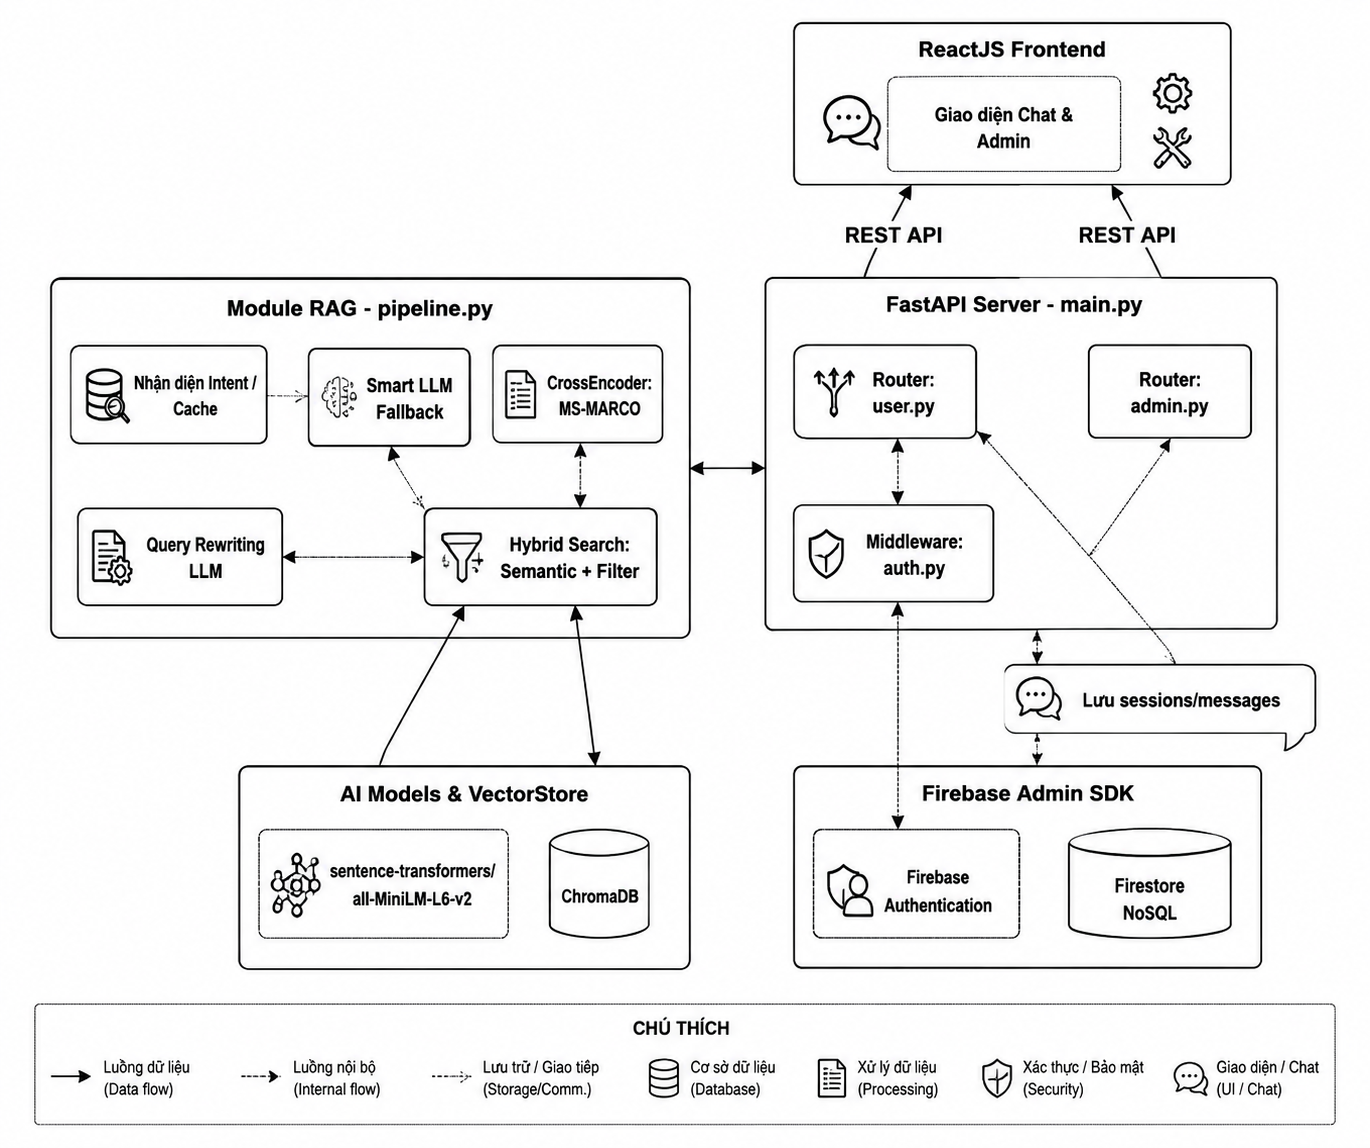
\includegraphics[width=0.92\textwidth]{tai_nguyen/media/image7.png}
\caption{Kiến trúc tổng thể của hệ thống chatbot RAG}
\label{fig:3-1}
\end{figure}

\section{Thiết kế mô hình lớp thực thể và
quan
hệ}

Để đáp ứng yêu cầu về Entity Class Diagram, hệ thống được mô hình hóa ở
mức thực thể nghiệp vụ thay vì chỉ trình bày bảng collection Firestore.
Các thực thể chính gồm User, Admin, Session, Message, Procedure,
ProcedureChunk, OTPCode, AdminSetting, BackupSetting và BackupRecord. Mô
hình này phản ánh cả dữ liệu người dùng, dữ liệu hội thoại, dữ liệu thủ
tục và dữ liệu vận hành vector database.

\begin{figure}[H]
\centering
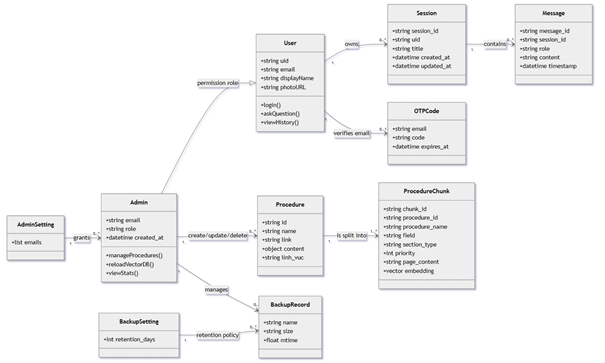
\includegraphics[width=0.92\textwidth]{tai_nguyen/media/image8.png}
\caption{Entity Class Diagram của hệ thống}
\label{fig:3-2}
\end{figure}

Quan hệ dữ liệu cốt lõi của hệ thống có thể hiểu như sau: một User có
nhiều Session; một Session có nhiều Message; một Procedure được chia
thành nhiều ProcedureChunk; Admin là người dùng có quyền đặc biệt để
quản lý Procedure và BackupRecord. ChromaDB không phải cơ sở dữ liệu
quan hệ, nhưng về thiết kế logic, mỗi chunk vẫn cần gắn với một thủ tục
thông qua procedure\_id để phục vụ truy xuất và trích dẫn nguồn.

\begin{figure}[H]
\centering
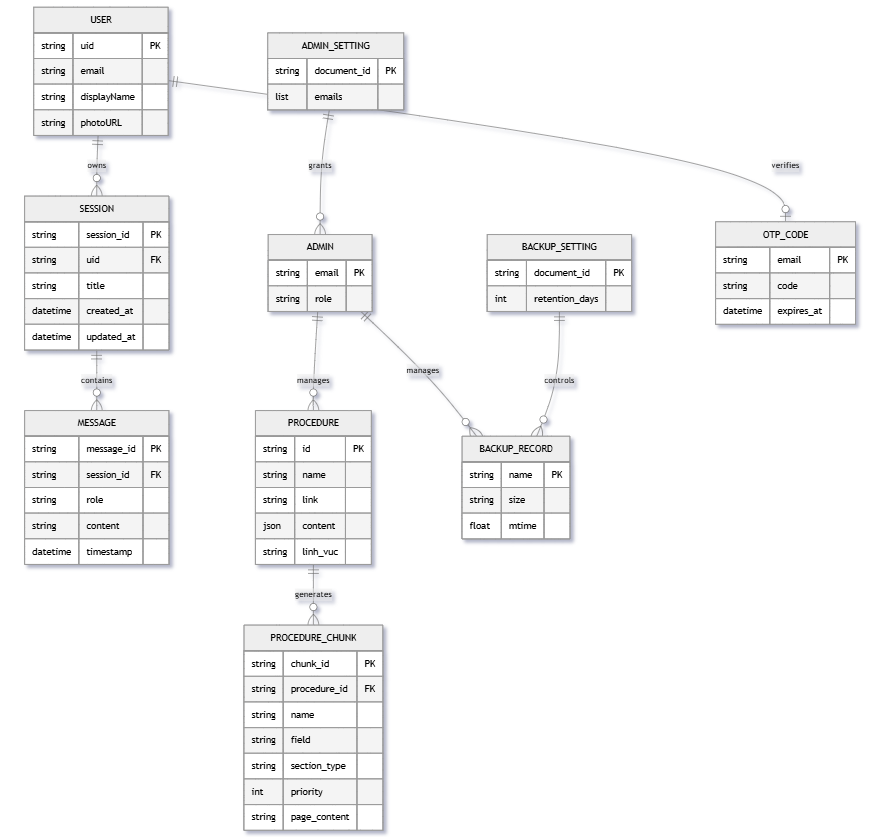
\includegraphics[width=0.92\textwidth]{tai_nguyen/media/image9.png}
\caption{Sơ đồ quan hệ dữ liệu User - Session - Message - Procedure - Chunk - Admin}
\label{fig:3-3}
\end{figure}

\begin{longtable}[]{|
  >{\raggedright\arraybackslash}p{(\columnwidth - 4\tabcolsep) * \real{0.2167}}|
  >{\raggedright\arraybackslash}p{(\columnwidth - 4\tabcolsep) * \real{0.3827}}|
  >{\raggedright\arraybackslash}p{(\columnwidth - 4\tabcolsep) * \real{0.4006}}|}
\caption{Thiết kế lớp thực thể chính}\\
\hline
\begin{minipage}[b]{\linewidth}\raggedright
\textbf{Lớp thực thể}
\end{minipage} & \begin{minipage}[b]{\linewidth}\raggedright
\textbf{Thuộc tính tiêu biểu}
\end{minipage} & \begin{minipage}[b]{\linewidth}\raggedright
\textbf{Vai trò}
\end{minipage} \\
\hline
\endfirsthead
\continuedcaption{Thiết kế lớp thực thể chính}
\hline
\begin{minipage}[b]{\linewidth}\raggedright
\textbf{Lớp thực thể}
\end{minipage} & \begin{minipage}[b]{\linewidth}\raggedright
\textbf{Thuộc tính tiêu biểu}
\end{minipage} & \begin{minipage}[b]{\linewidth}\raggedright
\textbf{Vai trò}
\end{minipage} \\
\hline
\endhead
\hline
\endlastfoot
User & uid, email, displayName, photoURL & Đại diện người dùng đã xác
thực qua Firebase. \\
\hline
Admin & email, role, created\_at & Người dùng có quyền truy cập
dashboard và API quản trị. \\
\hline
Session & session\_id, uid, title, created\_at, updated\_at & Phiên hội
thoại giữa người dùng và chatbot. \\
\hline
Message & message\_id, session\_id, role, content, timestamp & Tin nhắn
trong một phiên; role có thể là user hoặc bot. \\
\hline
Procedure & id, name, link, content, linh\_vuc & Thủ tục hành chính
trong procedures.json. \\
\hline
ProcedureChunk & chunk\_id, procedure\_id, field, section\_type,
priority, page\_content & Đoạn tri thức đã được chia nhỏ và lưu trong
ChromaDB. \\
\hline
OTPCode & email, code, expires\_at & Mã xác minh tạm thời khi đăng ký
tài khoản email. \\
\hline
BackupRecord & name, size, mtime & Bản sao lưu ChromaDB tạo trước khi
reload. \\
\hline
\end{longtable}

\section{Thiết kế cơ sở dữ
liệu}

Firestore và ChromaDB được sử dụng song song vì hai nhóm dữ liệu có bản
chất khác nhau. Firestore phù hợp với dữ liệu nghiệp vụ có định danh,
thời gian và quan hệ theo người dùng. ChromaDB phù hợp với dữ liệu văn
bản đã được nhúng thành vector để phục vụ tìm kiếm ngữ nghĩa. Thiết kế
này giúp hệ thống vừa quản lý được lịch sử hội thoại, vừa truy xuất được
dữ liệu thủ tục theo ý nghĩa câu hỏi.

Trong mã nguồn, lịch sử hội thoại được lưu theo collection sessions và
sub-collection messages. Hàm save\_message tạo hoặc cập nhật document
session, sau đó thêm từng tin nhắn vào sub-collection messages với role,
content và timestamp. Hàm get\_history chỉ lấy một số tin nhắn gần nhất
để đưa vào prompt, tránh làm prompt quá dài và giảm rủi ro đưa dư dữ
liệu cá nhân vào LLM.

\begin{longtable}[]{|
  >{\raggedright\arraybackslash}p{(\columnwidth - 4\tabcolsep) * \real{0.2921}}|
  >{\raggedright\arraybackslash}p{(\columnwidth - 4\tabcolsep) * \real{0.2929}}|
  >{\raggedright\arraybackslash}p{(\columnwidth - 4\tabcolsep) * \real{0.4150}}|}
\caption{Thiết kế các collection chính trên Firestore}\\
\hline
\begin{minipage}[b]{\linewidth}\raggedright
\textbf{Collection}
\end{minipage} & \begin{minipage}[b]{\linewidth}\raggedright
\textbf{Trường chính}
\end{minipage} & \begin{minipage}[b]{\linewidth}\raggedright
\textbf{Mục đích}
\end{minipage} \\
\hline
\endfirsthead
\continuedcaption{Thiết kế các collection chính trên Firestore}
\hline
\begin{minipage}[b]{\linewidth}\raggedright
\textbf{Collection}
\end{minipage} & \begin{minipage}[b]{\linewidth}\raggedright
\textbf{Trường chính}
\end{minipage} & \begin{minipage}[b]{\linewidth}\raggedright
\textbf{Mục đích}
\end{minipage} \\
\hline
\endhead
\hline
\endlastfoot
sessions & uid, title, created\_at, updated\_at & Lưu thông tin phiên
hội thoại. \\
\hline
sessions/\{id\}/messages & role, content, timestamp & Lưu từng tin nhắn
trong một phiên chat. \\
\hline
otp\_codes & code, expires\_at & Lưu OTP tạm thời, hết hạn sau 5
phút. \\
\hline
settings/admins & emails & Lưu danh sách email có quyền quản trị. \\
\hline
settings/backup & retention\_days & Lưu số ngày giữ backup ChromaDB. \\
\hline
\end{longtable}

Đối với ChromaDB, mỗi chunk lưu page\_content và metadata. Metadata được
tạo từ chunker.py, trong đó có procedure\_id, name, field,
section\_type, priority và chunk\_id. Các chunk được tạo theo nhóm tổng
quan, cách thức thực hiện, thành phần hồ sơ, căn cứ pháp lý và các
trường đơn giản. Với phí và lệ phí, chunker xử lý liên kết phí theo từng
hình thức thực hiện để tránh mất ngữ cảnh.

\begin{longtable}[]{|
  >{\raggedright\arraybackslash}p{(\columnwidth - 4\tabcolsep) * \real{0.2433}}|
  >{\raggedright\arraybackslash}p{(\columnwidth - 4\tabcolsep) * \real{0.2492}}|
  >{\raggedright\arraybackslash}p{(\columnwidth - 4\tabcolsep) * \real{0.5075}}|}
\caption{Thiết kế metadata cho dữ liệu trong ChromaDB}\\
\hline
\begin{minipage}[b]{\linewidth}\raggedright
\textbf{Trường metadata}
\end{minipage} & \begin{minipage}[b]{\linewidth}\raggedright
\textbf{Ý nghĩa}
\end{minipage} & \begin{minipage}[b]{\linewidth}\raggedright
\textbf{Ví dụ}
\end{minipage} \\
\hline
\endfirsthead
\continuedcaption{Thiết kế metadata cho dữ liệu trong ChromaDB}
\hline
\begin{minipage}[b]{\linewidth}\raggedright
\textbf{Trường metadata}
\end{minipage} & \begin{minipage}[b]{\linewidth}\raggedright
\textbf{Ý nghĩa}
\end{minipage} & \begin{minipage}[b]{\linewidth}\raggedright
\textbf{Ví dụ}
\end{minipage} \\
\hline
\endhead
\hline
\endlastfoot
procedure\_id / id & Mã thủ tục hành chính. & 2.002307.000.00.00.H35 \\
\hline
name / procedure\_name & Tên thủ tục. & Giải quyết chế độ mai táng phí
đối với cựu chiến binh \\
\hline
linh\_vuc & Lĩnh vực quản lý. & Người có công \\
\hline
field & Trường dữ liệu gốc. & Thành phần hồ sơ \\
\hline
section\_type & Loại chunk ngữ nghĩa. & summary, method, document,
legal, simple \\
\hline
chunk\_id & Định danh chunk. & 2.002307.000.00.00.H35\_document\_1 \\
\hline
priority & Mức ưu tiên khi truy xuất. & 10 \\
\hline
\end{longtable}

\section{Thiết kế pipeline RAG và trích dẫn
nguồn}

\begin{figure}[H]
\centering
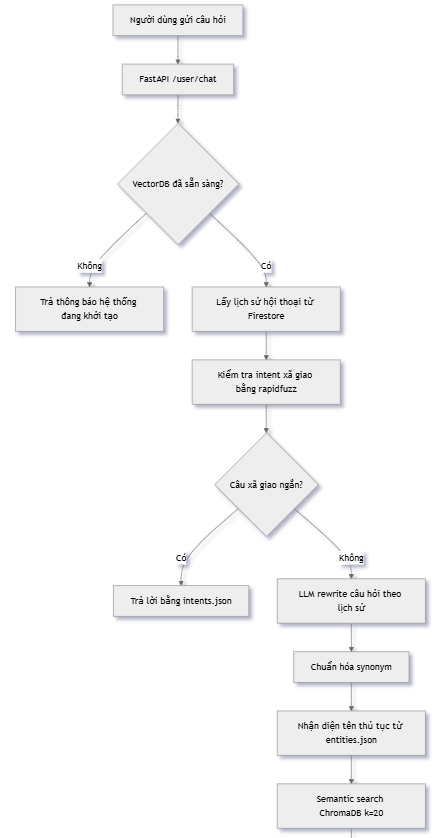
\includegraphics[height=0.74\textheight,keepaspectratio]{tai_nguyen/media/image10.png}
\caption{Luồng xử lý câu hỏi bằng pipeline RAG (a)}
\label{fig:3-4}
\end{figure}
Pipeline
RAG gồm hai pha: nạp dữ liệu và hỏi đáp. Pha nạp dữ liệu đọc
procedures.json, làm sạch văn bản, chia semantic chunks, gắn metadata,
sinh embedding và lưu vào ChromaDB. Pha hỏi đáp nhận câu hỏi của người
dùng, lấy lịch sử gần nhất, xử lý intent, rewrite câu hỏi nếu cần, chuẩn
hóa synonym, truy xuất ChromaDB, rerank bằng CrossEncoder, chọn context
và gọi LLM để sinh câu trả lời.

Trong code hiện tại, endpoint chat gọi ask\_rag với db, query,
session\_id và history. Bên trong pipeline, câu hỏi ngắn thuộc nhóm xã
giao được handle\_intent xử lý sớm. Nếu là câu nghiệp vụ, hệ thống có
thể dùng LLM nhẹ để rewrite câu hỏi dựa trên lịch sử, sau đó
normalize\_query, detect\_procedure\_name và detect\_field. Retrieval
gồm semantic search k=20 và truy xuất bổ sung có filter theo tên thủ tục
k=10 nếu nhận diện được thủ tục. Các tài liệu được loại trùng, rerank
bằng CrossEncoder và chọn tối đa 10 chunk làm context.

\begin{figure}[H]
\centering
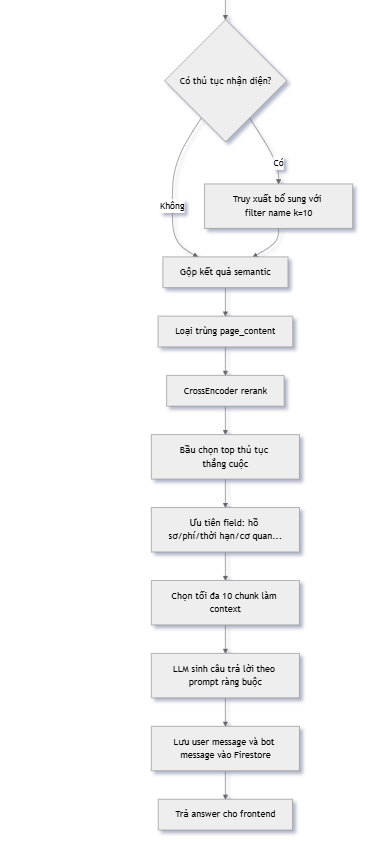
\includegraphics[height=0.74\textheight,keepaspectratio]{tai_nguyen/media/image11.png}
\caption{Luồng xử lý câu hỏi bằng pipeline RAG (b)}
\label{fig:3-5}
\end{figure}
Để
khắc phục hạn chế về việc chưa hiển thị nguồn chi tiết cho từng câu trả
lời, hệ thống có thể được mở rộng thêm cơ chế trích dẫn nguồn. Theo
thiết kế đề xuất, kết quả trả về của pipeline RAG không chỉ gồm nội dung
trả lời mà còn kèm danh sách nguồn dữ liệu đã được sử dụng trong quá
trình sinh câu trả lời.

Danh sách nguồn có thể được lấy từ metadata của các chunk sau bước truy
xuất, rerank và lọc theo trường thông tin. Mỗi nguồn gồm các thông tin
như mã thủ tục, tên thủ tục, mục dữ liệu được sử dụng, mã chunk và đường
dẫn trang nguồn nếu dữ liệu gốc có cung cấp. Khi hiển thị trên giao
diện, frontend có thể đặt phần ``Nguồn tham khảo'' ở cuối câu trả lời để
người dùng kiểm chứng lại thông tin.

Cách thiết kế này giúp tăng tính minh bạch của chatbot hành chính công.
Người dân có thể biết câu trả lời được tổng hợp từ thủ tục nào, còn quản
trị viên có thêm căn cứ để kiểm tra khi hệ thống truy xuất nhầm chunk
hoặc dữ liệu nguồn chưa được chuẩn hóa tốt.

\begin{figure}[H]
\centering
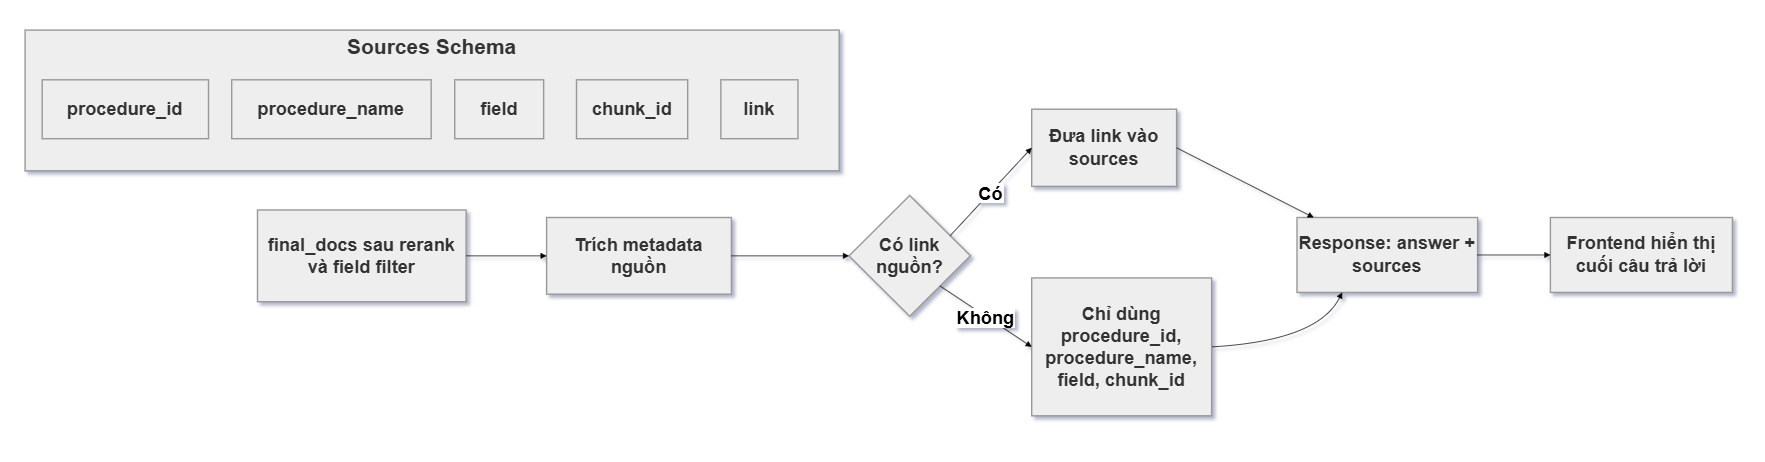
\includegraphics[width=0.92\textwidth]{tai_nguyen/media/image12.png}
\caption{Thiết kế trích dẫn nguồn trong câu trả lời}
\label{fig:3-6}
\end{figure}

\begin{longtable}{|>{\raggedright\arraybackslash}p{0.27\textwidth}|>{\raggedright\arraybackslash}p{0.35\textwidth}|>{\raggedright\arraybackslash}p{0.30\textwidth}|}
\caption{Thiết kế nguồn trích dẫn trong câu trả lời}\\
\hline
\textbf{Trường} & \textbf{Mô tả} & \textbf{Ví dụ} \\
\hline
\endfirsthead
\continuedcaption{Thiết kế nguồn trích dẫn trong câu trả lời}
\hline
\textbf{Trường} & \textbf{Mô tả} & \textbf{Ví dụ} \\
\hline
\endhead
\hline
\endlastfoot
\codepathraw{answer} & Câu trả lời cuối cùng của chatbot. & Hồ sơ gồm... \\
\hline
\codepath{sources[].procedure_id} & Mã thủ tục dùng làm nguồn. & \codepathraw{2.002307.000.00.00.H35} \\
\hline
\codepath{sources[].procedure_name} & Tên thủ tục dùng làm nguồn. & Giải quyết chế độ mai táng phí đối với cựu chiến binh \\
\hline
\codepath{sources[].field} & Mục thông tin được sử dụng. & Thành phần hồ sơ \\
\hline
\codepath{sources[].chunk_id} & Chunk cụ thể trong ChromaDB. & \codepathraw{2.002307.000.00.00.H35_document_1} \\
\hline
\codepath{sources[].link} & Đường dẫn trang nguồn nếu có. & URL trang chi tiết thủ tục \\
\hline
\end{longtable}

\section{Thiết kế API và request/response
mẫu}

API của hệ thống được chia thành ba nhóm chính: auth, user và admin.
Nhóm auth phục vụ xác thực người dùng, gửi OTP và kiểm tra quyền quản
trị; nhóm user phục vụ các chức năng phía người dân như hỏi đáp chatbot,
lấy danh sách phiên và xem lịch sử hội thoại; nhóm admin phục vụ thống
kê, quản lý dữ liệu thủ tục, chuyển văn bản sang JSON, quản lý backup và
đồng bộ lại vector database. Cách tách nhóm API này giúp backend kiểm
soát quyền truy cập rõ ràng, đồng thời giúp frontend gọi đúng nhóm chức
năng theo vai trò người dùng.

Trong mã nguồn hiện tại, endpoint /user/chat đang được cài đặt bằng
phương thức GET với tham số q và session\_id. Endpoint này kiểm tra
token Firebase, lấy lịch sử hội thoại, gọi pipeline RAG, sau đó lưu tin
nhắn của người dùng và câu trả lời của bot vào Firestore bằng background
task. Tuy nhiên, nếu xét theo thiết kế REST hoàn thiện, nghiệp vụ gửi
câu hỏi nên chuyển sang POST vì request có nội dung nghiệp vụ, cần xác
thực, có thể truyền body JSON và phát sinh tác động ghi lịch sử hội
thoại. Do đó, phần thiết kế dưới đây ghi rõ cả hiện trạng mã nguồn và
phương án đề xuất để thuận lợi khi nâng cấp.

Ngoài API hỏi đáp chatbot, hệ thống nên bổ sung thêm hai API phía người
dùng để bám đầy đủ Use Case tra cứu thủ tục và xem chi tiết thông tin
thủ tục. Trong phiên bản hiện tại, người dùng chủ yếu tra cứu qua
chatbot RAG; dữ liệu thủ tục đầy đủ đang được quản lý ở phía admin thông
qua /admin/documents. Khi hoàn thiện sản phẩm, có thể bổ sung GET
/user/procedures để tra cứu danh sách thủ tục và GET
/user/procedures/\{procedure\_id\} để xem chi tiết một thủ tục cụ thể.
Hai API này không thay thế chatbot mà đóng vai trò bổ trợ, giúp người
dùng có thêm cách tiếp cận dữ liệu theo kiểu tra cứu truyền thống.

\begin{longtable}[]{|
  >{\raggedright\arraybackslash}p{(\columnwidth - 6\tabcolsep) * \real{0.0985}}|
  >{\raggedright\arraybackslash}p{(\columnwidth - 6\tabcolsep) * \real{0.3805}}|
  >{\raggedright\arraybackslash}p{(\columnwidth - 6\tabcolsep) * \real{0.3196}}|
  >{\raggedright\arraybackslash}p{(\columnwidth - 6\tabcolsep) * \real{0.2014}}|}
\caption{Danh sách API chính và API đề xuất của hệ thống}\\
\hline
\begin{minipage}[b]{\linewidth}\raggedright
\textbf{Nhóm}
\end{minipage} & \begin{minipage}[b]{\linewidth}\raggedright
\textbf{Endpoint}
\end{minipage} & \begin{minipage}[b]{\linewidth}\raggedright
\textbf{Phương thức thiết kế}
\end{minipage} & \begin{minipage}[b]{\linewidth}\raggedright
\textbf{Chức năng / Ghi chú}
\end{minipage} \\
\hline
\endfirsthead
\continuedcaption{Danh sách API chính và API đề xuất của hệ thống}
\hline
\begin{minipage}[b]{\linewidth}\raggedright
\textbf{Nhóm}
\end{minipage} & \begin{minipage}[b]{\linewidth}\raggedright
\textbf{Endpoint}
\end{minipage} & \begin{minipage}[b]{\linewidth}\raggedright
\textbf{Phương thức thiết kế}
\end{minipage} & \begin{minipage}[b]{\linewidth}\raggedright
\textbf{Chức năng / Ghi chú}
\end{minipage} \\
\hline
\endhead
\hline
\endlastfoot
Auth & /auth/check-admin & GET & Kiểm tra tài khoản hiện tại có quyền
admin hay không. \\
\hline
Auth & /auth/send-otp & POST & Sinh và lưu OTP cho email đăng ký. \\
\hline
Auth & /auth/verify-otp & POST & Xác minh OTP và tạo tài khoản
Firebase. \\
\hline
User & /user/chat & POST đề xuất; code hiện tại GET & Gửi câu hỏi đến
chatbot, nhận câu trả lời và lưu lịch sử hội thoại. \\
\hline
User & /user/sessions & GET & Lấy danh sách phiên chat theo người dùng
đã đăng nhập. \\
\hline
User & /user/chat/history & GET & Lấy lịch sử tin nhắn của một
session. \\
\hline
User & /user/procedures & GET đề xuất & Tra cứu danh sách thủ tục theo
từ khóa, lĩnh vực hoặc tên gần đúng. \\
\hline
User & /user/procedures/\{procedure\_id\} & GET đề xuất & Lấy chi tiết
một thủ tục hành chính theo mã thủ tục. \\
\hline
Admin & /admin/documents & GET/POST/PUT/DELETE & Quản lý dữ liệu thủ tục
hành chính trong procedures.json. \\
\hline
Admin & /admin/reload-vectordb & POST & Build lại ChromaDB từ dữ liệu
procedures.json và tạo backup trước khi build. \\
\hline
Admin & /admin/backups & GET/DELETE & Quản lý bản sao lưu vector
database. \\
\hline
Admin & /admin/convert-json & POST & Dùng AI chuyển văn bản thủ tục thô
thành JSON. \\
\hline
\end{longtable}

\begin{enumerate}
\def\labelenumi{\arabic{enumi}.}
\item
  \textbf{Thiết kế API tra cứu và xem chi tiết thủ tục}
\end{enumerate}

Luồng tra cứu thủ tục cho phép người dùng nhập từ khóa hoặc mô tả nhu
cầu đời thường để tìm các thủ tục liên quan. Backend có thể tìm theo tên
thủ tục, lĩnh vực, metadata hoặc kết hợp với dữ liệu đã chuẩn hóa trong
entities.json. Kết quả trả về nên gồm các thông tin ngắn như mã thủ tục,
tên thủ tục, lĩnh vực và đường dẫn nguồn nếu có. Sau đó, người dùng có
thể chọn một thủ tục để xem chi tiết theo từng nhóm thông tin.

GET /user/procedures?keyword=nuôi con nuôi\&limit=10\\
Authorization: Bearer \textless Firebase\_ID\_Token\textgreater{}\\
\strut \\
Response body:\\
\{\\
"procedures": {[}\\
\{\\
"id": "2.002307.000.00.00.H35",\\
"name": "Đăng ký việc nuôi con nuôi trong nước",\\
"linh\_vuc": "Nuôi con nuôi",\\
"link": "URL trang nguồn nếu có"\\
\}\\
{]}\\
\}

Luồng xem chi tiết thủ tục được thiết kế để trả về đầy đủ dữ liệu của
một thủ tục cụ thể. API này phù hợp với Use Case ``Xem chi tiết thông
tin thủ tục'' đã tách ở Chương 2. Khi nhận procedure\_id, backend tìm
bản ghi tương ứng trong procedures.json và trả về các trường như thành
phần hồ sơ, thời hạn giải quyết, cơ quan thực hiện, phí, lệ phí, kết quả
và căn cứ pháp lý. Nếu không tìm thấy mã thủ tục, hệ thống cần trả thông
báo lỗi rõ ràng để frontend hiển thị cho người dùng.

GET /user/procedures/2.002307.000.00.00.H35\\
Authorization: Bearer \textless Firebase\_ID\_Token\textgreater{}\\
\strut \\
Response body:\\
\{\\
"id": "2.002307.000.00.00.H35",\\
"name": "Đăng ký việc nuôi con nuôi trong nước",\\
"link": "URL trang nguồn nếu có",\\
"content": \{\\
"Lĩnh vực": "Nuôi con nuôi",\\
"Thành phần hồ sơ": {[}{]},\\
"Thời hạn giải quyết": "...",\\
"Cơ quan thực hiện": "...",\\
"Phí": {[}{]},\\
"Lệ phí": {[}{]},\\
"Kết quả thực hiện": "...",\\
"Căn cứ pháp lý": {[}{]}\\
\}\\
\}

\begin{figure}[H]
\centering
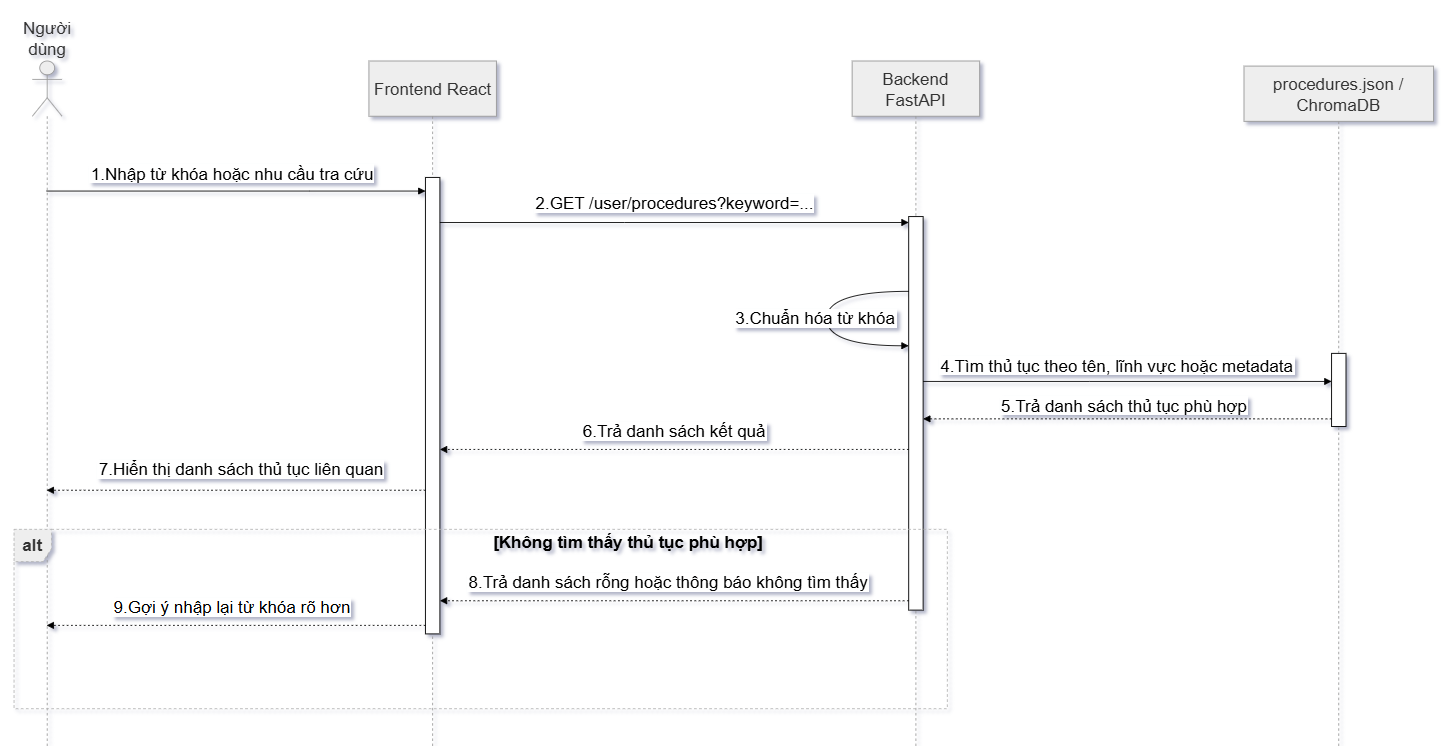
\includegraphics[width=0.92\textwidth]{tai_nguyen/media/image13.png}
\caption{Sơ đồ tuần tự luồng tra cứu TTHC}
\label{fig:3-7}
\end{figure}

\begin{figure}[H]
\centering
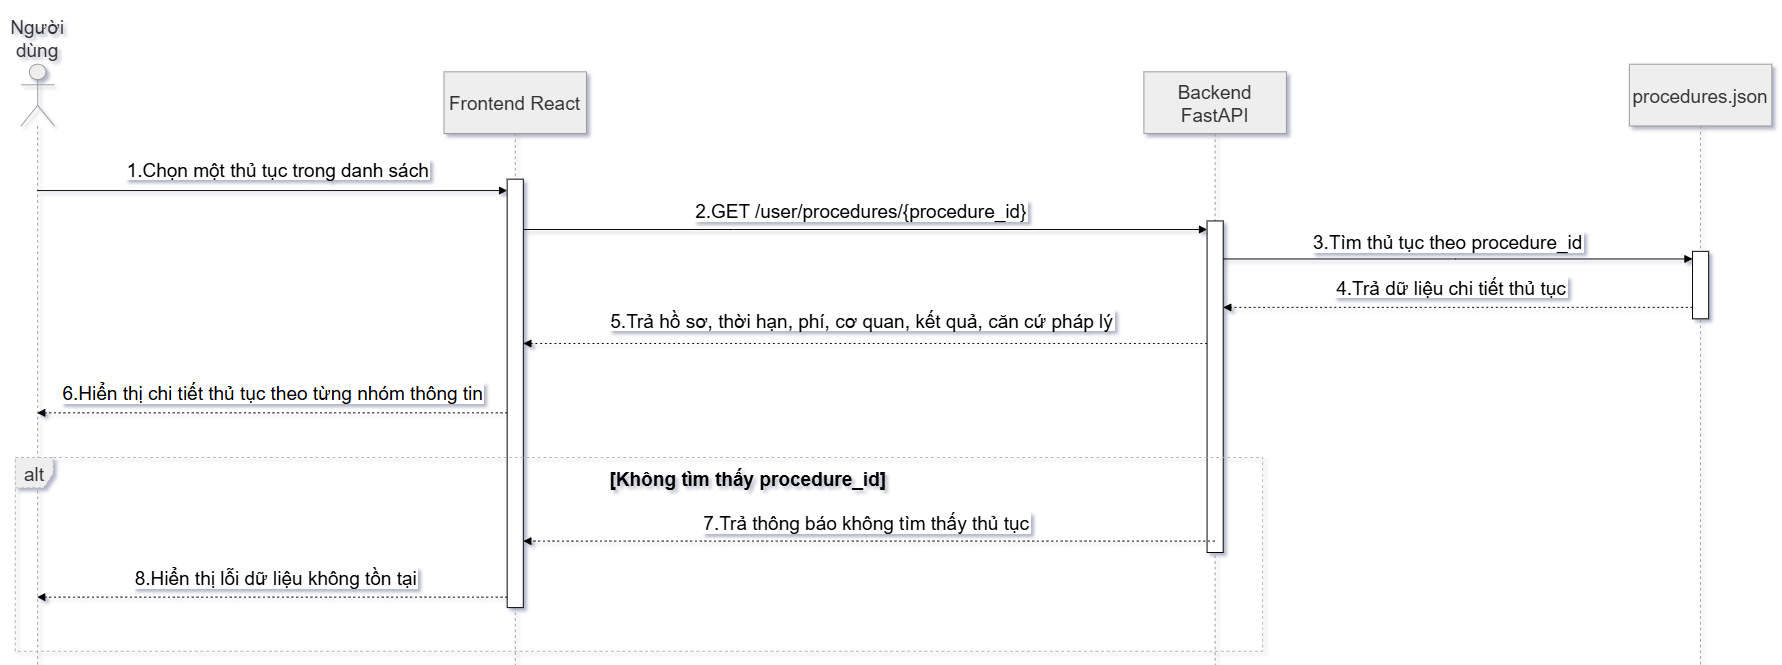
\includegraphics[width=0.92\textwidth]{tai_nguyen/media/image14.png}
\caption{Sơ đồ tuần tự luồng xem chi tiết thông tin thủ tục}
\label{fig:3-8}
\end{figure}

\begin{enumerate}
\def\labelenumi{\arabic{enumi}.}
\setcounter{enumi}{1}
\item
  \textbf{Thiết kế API hỏi đáp chatbot RAG}
\end{enumerate}

API /user/chat là luồng quan trọng nhất vì kết nối trực tiếp giao diện
hội thoại với pipeline RAG. Với thiết kế đề xuất, frontend gửi câu hỏi
và session\_id trong body JSON. Backend xác thực Firebase ID Token, lấy
lịch sử hội thoại gần nhất, gọi ask\_rag để tạo câu trả lời, sau đó lưu
tin nhắn vào Firestore. Response nên mở rộng thêm trường sources để hỗ
trợ trích dẫn nguồn trong tương lai.

\begin{figure}[H]
\centering
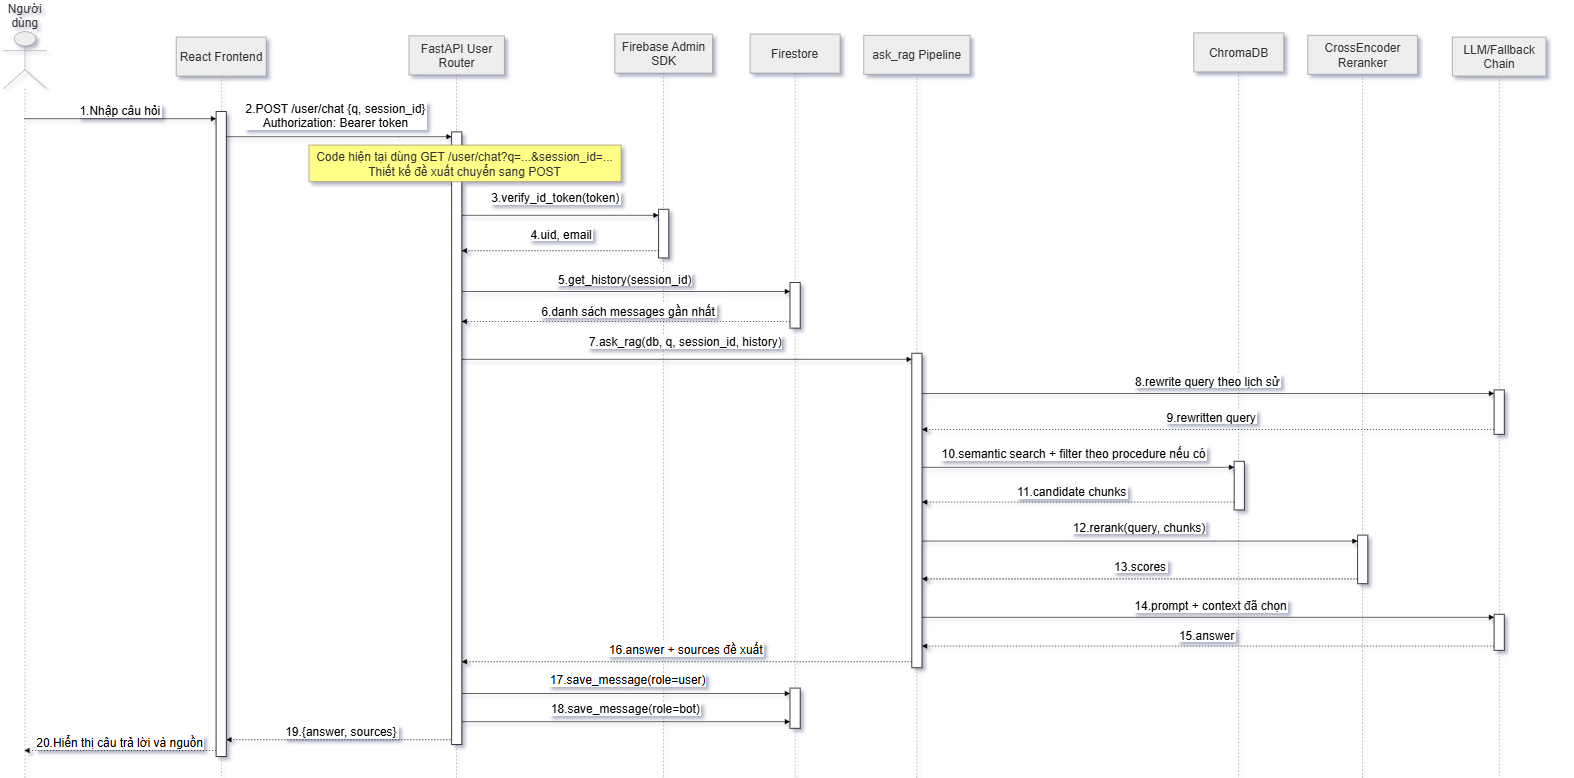
\includegraphics[width=0.92\textwidth]{tai_nguyen/media/image15.png}
\caption{Sơ đồ tuần tự xử lý API /user/chat}
\label{fig:3-9}
\end{figure}

\begin{enumerate}
\def\labelenumi{\arabic{enumi}.}
\setcounter{enumi}{2}
\item
  \textbf{Thiết kế API quản lý tài liệu và đồng bộ VectorDB}
\end{enumerate}

Nhóm API quản trị được bảo vệ bằng quyền admin ở backend. API
/admin/documents phục vụ xem, thêm, sửa, xóa dữ liệu thủ tục trong
procedures.json. Sau khi dữ liệu thay đổi, admin cần gọi
/admin/reload-vectordb để hệ thống đọc lại dữ liệu, tạo semantic chunks,
backup ChromaDB cũ và build lại vector database mới. Đây là luồng quan
trọng để kho tri thức của chatbot luôn đồng bộ với dữ liệu nguồn.

\begin{figure}[H]
\centering
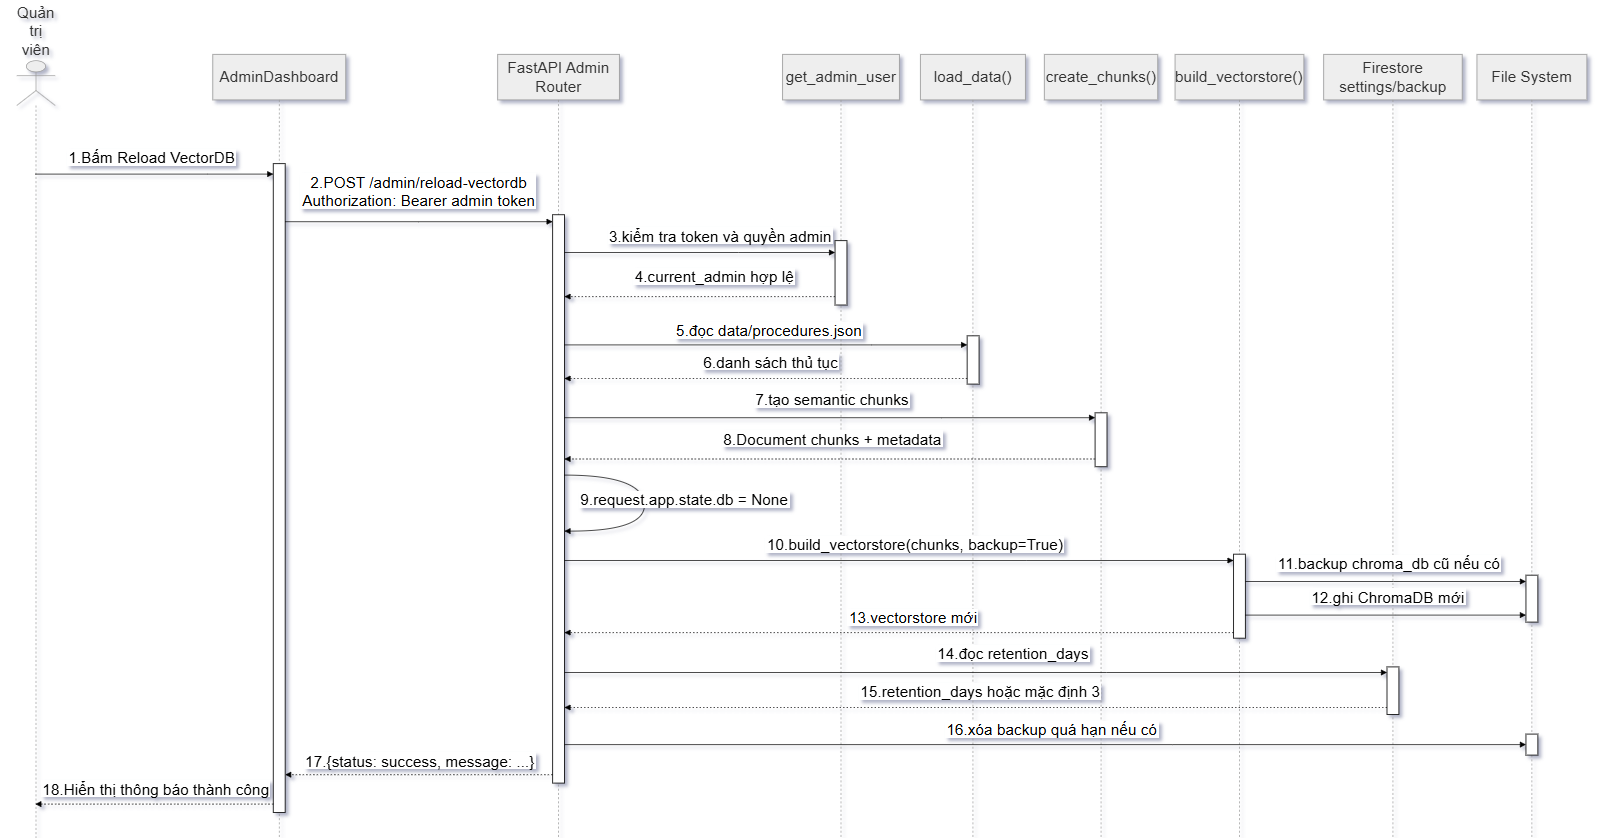
\includegraphics[width=0.92\textwidth]{tai_nguyen/media/image16.png}
\caption{Sơ đồ tuần tự đồng bộ VectorDB}
\label{fig:3-10}
\end{figure}

Như vậy, phần thiết kế API cần phân biệt rõ ba mức: API đã có trong mã
nguồn hiện tại, API nên chuyển đổi để đúng REST hơn và API đề xuất để
hoàn thiện Use Case tra cứu/xem chi tiết thủ tục. Cách trình bày này
giúp báo cáo vừa trung thực với code đã triển khai, vừa thể hiện được
hướng hoàn thiện hợp lý cho hệ thống.

\section{Thiết kế giao diện người dùng và
quản
trị}

Giao diện người dùng lấy khung hội thoại làm trung tâm. Người dân nhìn
thấy danh sách tin nhắn, ô nhập câu hỏi, câu hỏi gợi ý và sidebar lịch
sử. Khi câu trả lời dài, hệ thống ưu tiên xuống dòng và gạch đầu dòng để
người dùng dễ đọc trên điện thoại. Giao diện quản trị được tổ chức theo
tab để tách các nhóm chức năng: thống kê, lịch sử, tài liệu, backup và
quản lý admin.

Các component React phản ánh đúng trách nhiệm giao diện. App điều phối
trạng thái đăng nhập và phân quyền; LoginPage xử lý đăng nhập, đăng ký
và OTP; ChatBox điều phối hội thoại; Sidebar hiển thị session; InputBox
nhập câu hỏi; Message hiển thị tin nhắn; AdminDashboard phục vụ thao tác
quản trị. Cách chia component này giúp giao diện dễ bảo trì và dễ mở
rộng.

\begin{figure}[H]
\centering
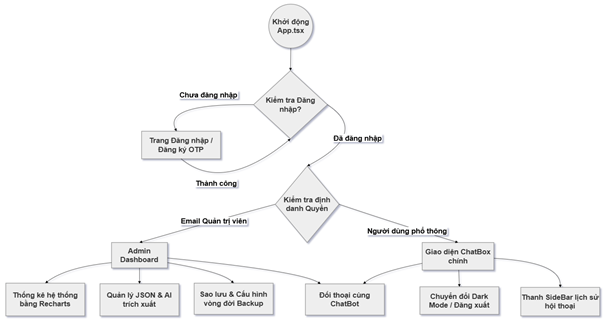
\includegraphics[width=0.92\textwidth]{tai_nguyen/media/image17.png}
\caption{Sitemap giao diện người dùng và quản trị viên thiết kế bảo mật và phân quyền}
\label{fig:3-11}
\end{figure}

\begin{figure}[H]
\centering
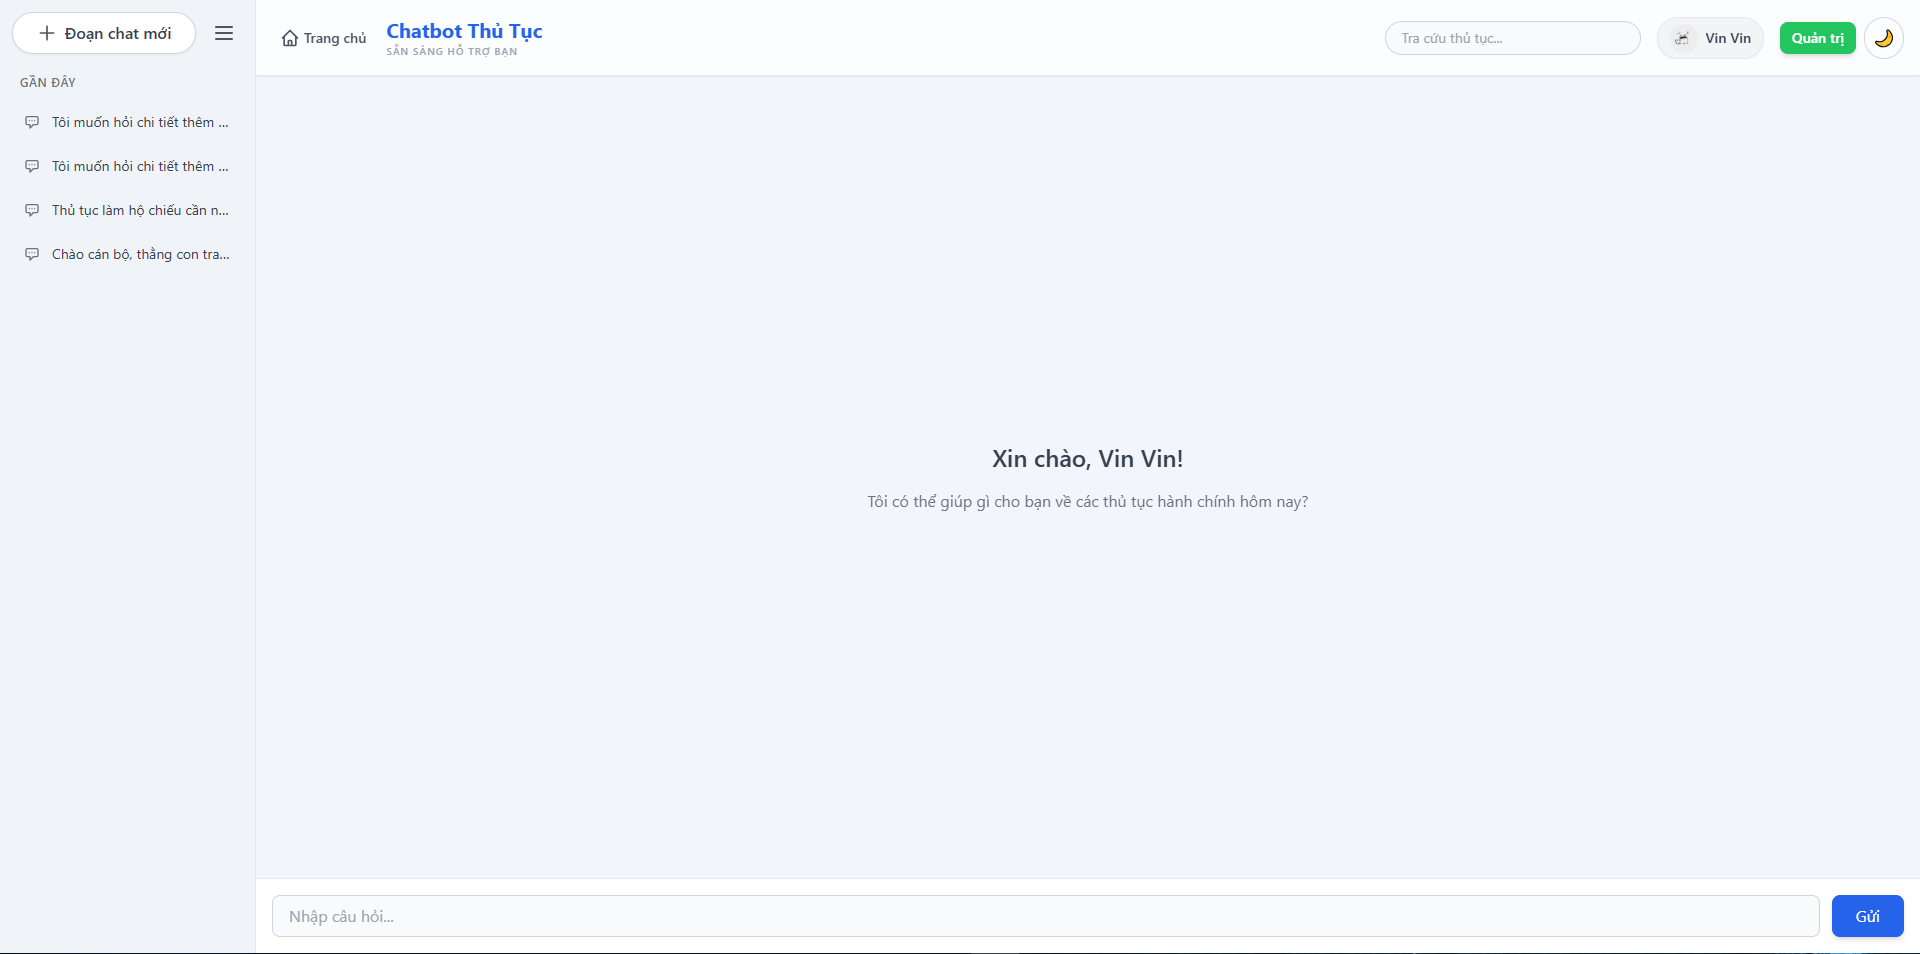
\includegraphics[width=0.92\textwidth]{tai_nguyen/media/image18.png}
\caption{Giao diện hỏi đáp TTHC bằng chatbot}
\label{fig:3-12}
\end{figure}

\begin{figure}[H]
\centering
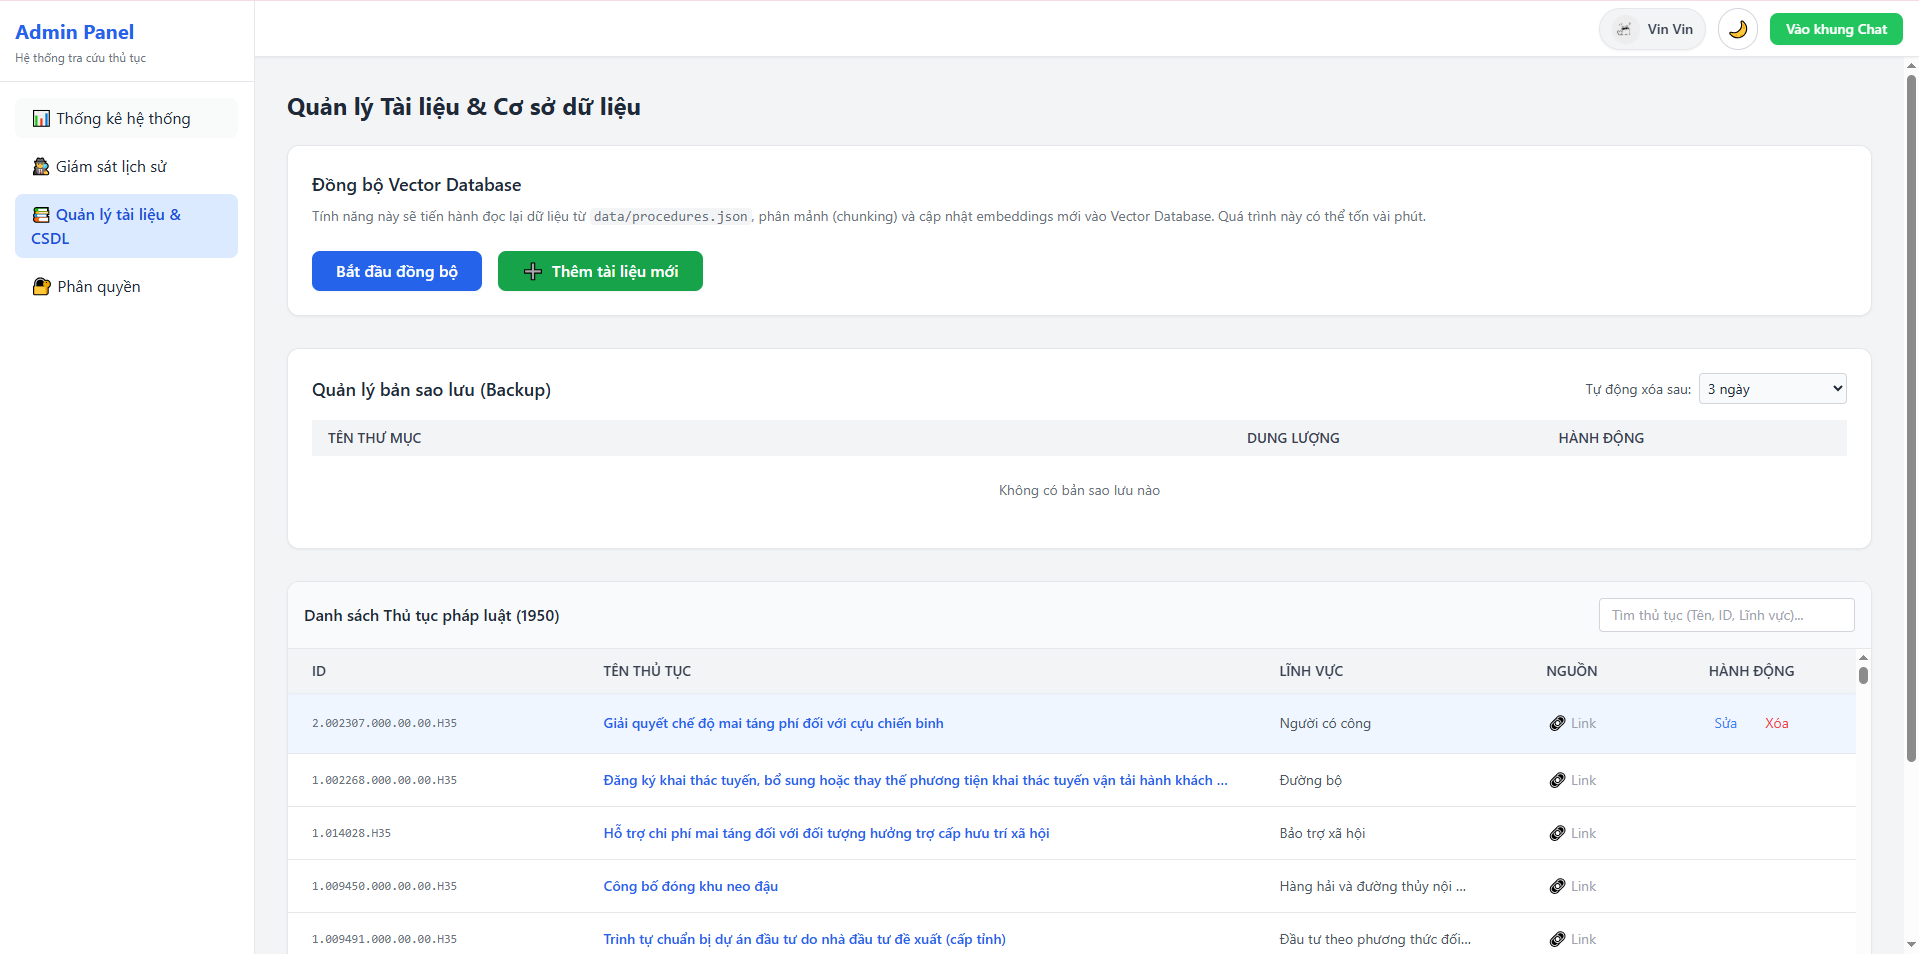
\includegraphics[width=0.92\textwidth]{tai_nguyen/media/image19.png}
\caption{Giao diện quản lý dữ liệu TTHC}
\label{fig:3-13}
\end{figure}

Bảo mật được kiểm soát chủ yếu ở backend. Frontend lấy Firebase ID Token
sau khi đăng nhập và gửi trong header Authorization. Backend dùng
Firebase Admin SDK để xác minh token. Với các endpoint /admin, backend
tiếp tục kiểm tra email trong danh sách admin hoặc custom claim thông
qua dependency get\_admin\_user. Cách làm này tránh tình trạng người
dùng chỉ cần sửa giao diện là truy cập được chức năng quản trị.

Dữ liệu nhạy cảm như serviceAccountKey, API key, sender password và
token không được đưa vào frontend. Các giá trị này cần đặt trong .env
hoặc secret của môi trường triển khai. Với ChromaDB, trước khi reload dữ
liệu cần backup thư mục cũ; sau khi build lại, hệ thống có thể dọn
backup quá hạn theo retention\_days để tránh tăng dung lượng không kiểm
soát.

Bảo mật RAG cũng được thiết kế ở tầng prompt. Mô hình chỉ được trả lời
theo context đã truy xuất; nếu dữ liệu không có, chatbot phải từ chối
trả lời thay vì suy đoán. Đây vừa là yêu cầu kỹ thuật, vừa là yêu cầu
nghiệp vụ trong hệ thống hành chính công.

\section{Thiết kế triển khai và cấu trúc mã
nguồn}

Hệ thống được triển khai theo kiến trúc web tách lớp. Người dùng thao
tác trên trình duyệt hoặc thiết bị di động thông qua giao diện React.
Backend FastAPI tiếp nhận request, xác thực người dùng, điều phối
pipeline RAG, gọi mô hình AI và ghi dữ liệu vận hành. Firebase
Authentication và Firestore phục vụ xác thực, lưu session, tin nhắn, OTP
và cấu hình quản trị. ChromaDB lưu vector embedding cùng metadata của
các đoạn dữ liệu TTHC.

\begin{figure}[H]
\centering
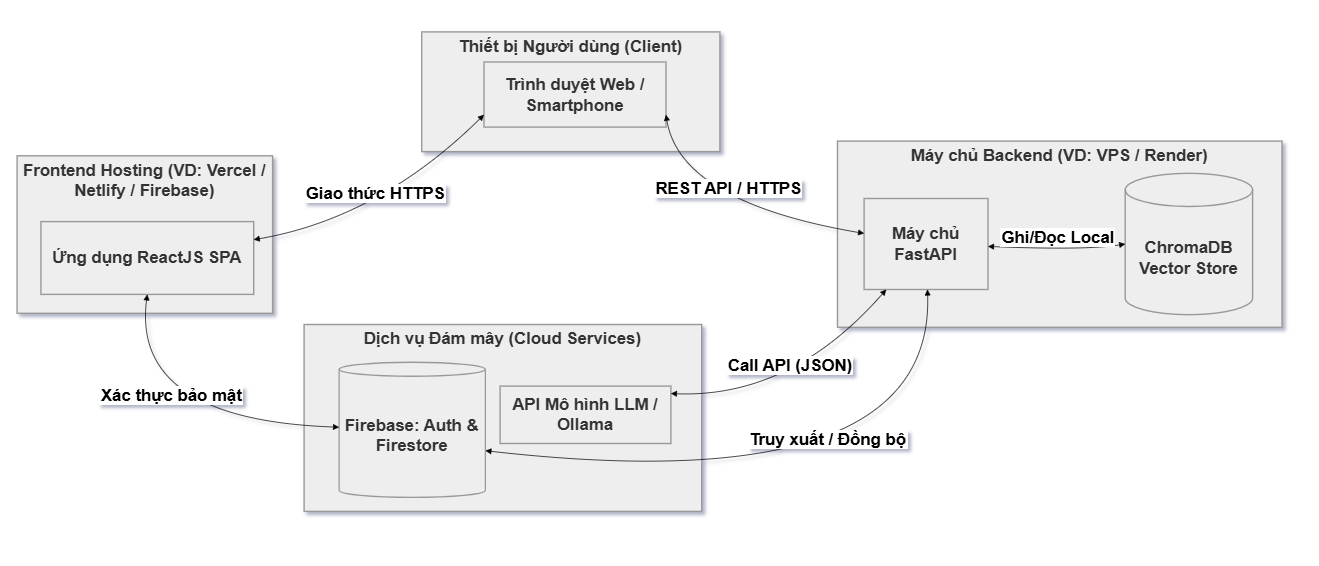
\includegraphics[width=0.92\textwidth]{tai_nguyen/media/image20.png}
\caption{Biểu đồ triển khai hệ thống (Deployment Diagram)}
\label{fig:3-14}
\end{figure}

Trong phạm vi thử nghiệm của đồ án, backend được khởi chạy bằng Uvicorn
trên cổng 8000. Khi cần truy cập từ môi trường bên ngoài hoặc demo trên
thiết bị khác, backend được mở ra Internet thông qua tunnel ngrok.
Frontend chạy bằng Vite và kết nối tới API URL tương ứng với backend
đang hoạt động.

\begin{longtable}[]{|
  >{\raggedright\arraybackslash}p{(\columnwidth - 4\tabcolsep) * \real{0.1514}}|
  >{\raggedright\arraybackslash}p{(\columnwidth - 4\tabcolsep) * \real{0.2659}}|
  >{\raggedright\arraybackslash}p{(\columnwidth - 4\tabcolsep) * \real{0.5827}}|}
\caption{Môi trường và thành phần triển khai}\\
\hline
\begin{minipage}[b]{\linewidth}\raggedright
\textbf{Thành phần}
\end{minipage} & \begin{minipage}[b]{\linewidth}\raggedright
\textbf{Công nghệ/công cụ}
\end{minipage} & \begin{minipage}[b]{\linewidth}\raggedright
\textbf{Vai trò}
\end{minipage} \\
\hline
\endfirsthead
\continuedcaption{Môi trường và thành phần triển khai}
\hline
\begin{minipage}[b]{\linewidth}\raggedright
\textbf{Thành phần}
\end{minipage} & \begin{minipage}[b]{\linewidth}\raggedright
\textbf{Công nghệ/công cụ}
\end{minipage} & \begin{minipage}[b]{\linewidth}\raggedright
\textbf{Vai trò}
\end{minipage} \\
\hline
\endhead
\hline
\endlastfoot
Backend & Python, FastAPI, Uvicorn & Cung cấp API, xác thực token, xử lý
RAG và quản trị dữ liệu. \\
\hline
Frontend & React, TypeScript, Vite & Xây dựng giao diện chatbot, đăng
nhập, lịch sử và dashboard quản trị. \\
\hline
Giao diện & Tailwind CSS, Recharts & Thiết kế responsive, dark mode và
biểu đồ thống kê. \\
\hline
AI/RAG & Ollama/Qwen, Gemini/OpenRouter, CrossEncoder & Rewrite câu hỏi,
truy xuất, rerank, sinh phản hồi và fallback. \\
\hline
Vector DB & ChromaDB & Lưu embedding và metadata của từng chunk thủ
tục. \\
\hline
Dữ liệu cloud & Firebase Authentication, Firestore & Xác thực, lưu lịch
sử chat, OTP, settings và danh sách admin. \\
\hline
\end{longtable}

\begin{longtable}[]{|
  >{\raggedright\arraybackslash}p{(\columnwidth - 4\tabcolsep) * \real{0.1949}}|
  >{\raggedright\arraybackslash}p{(\columnwidth - 4\tabcolsep) * \real{0.2773}}|
  >{\raggedright\arraybackslash}p{(\columnwidth - 4\tabcolsep) * \real{0.5278}}|}
\caption{Nhóm mã nguồn backend và vai trò}\\
\hline
\begin{minipage}[b]{\linewidth}\raggedright
\textbf{Nhóm}
\end{minipage} & \begin{minipage}[b]{\linewidth}\raggedright
\textbf{File tiêu biểu}
\end{minipage} & \begin{minipage}[b]{\linewidth}\raggedright
\textbf{Vai trò}
\end{minipage} \\
\hline
\endfirsthead
\continuedcaption{Nhóm mã nguồn backend và vai trò}
\hline
\begin{minipage}[b]{\linewidth}\raggedright
\textbf{Nhóm}
\end{minipage} & \begin{minipage}[b]{\linewidth}\raggedright
\textbf{File tiêu biểu}
\end{minipage} & \begin{minipage}[b]{\linewidth}\raggedright
\textbf{Vai trò}
\end{minipage} \\
\hline
\endhead
\hline
\endlastfoot
Khởi động ứng dụng & main.py & Khởi tạo FastAPI, Firebase, CORS, router
và load/build ChromaDB. \\
\hline
Xử lý dữ liệu & loader.py, chunker.py, vectorstore.py & Đọc
procedures.json, chia chunk và lưu embedding vào ChromaDB. \\
\hline
Hỏi đáp RAG & pipeline.py, normalizer.py, intent.py & Chuẩn hóa câu hỏi,
nhận diện intent, retrieval, rerank, prompt và gọi LLM. \\
\hline
Bộ nhớ hội thoại & memory.py & Đọc và ghi lịch sử chat theo session
trong Firestore. \\
\hline
Router API & auth.py, user.py, admin.py & Xác thực, chat người dùng,
quản trị dữ liệu, backup và reload VectorDB. \\
\hline
\end{longtable}

Bảng 3.7 chỉ trình bày các nhóm mã nguồn chính để người đọc nắm được cấu
trúc triển khai. Cấu trúc thư mục backend và frontend được trình bày cụ
thể tại Phụ lục A.

\begin{figure}[H]
\centering
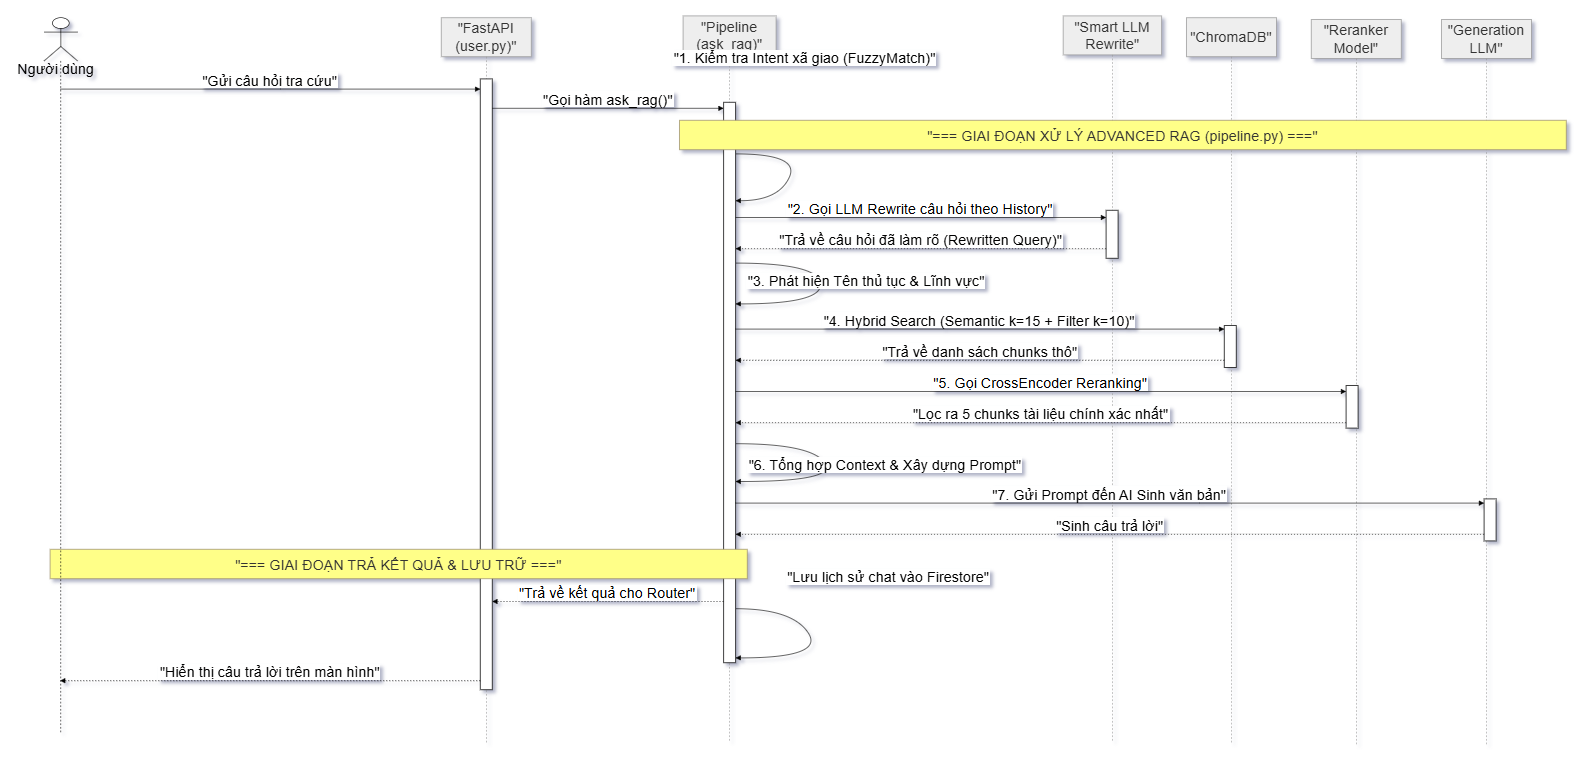
\includegraphics[width=0.92\textwidth]{tai_nguyen/media/image21.png}
\caption{Sơ đồ tuần tự xử lý Pipeline Advanced RAG chi tiết}
\label{fig:3-15}
\end{figure}

Khi backend khởi động, hệ thống ưu tiên nạp ChromaDB đã tồn tại. Nếu
chưa có vector database, backend đọc procedures.json, tạo semantic
chunks, sinh embedding và lưu vào ChromaDB. Trong quá trình hỏi đáp,
pipeline xử lý intent, viết lại câu hỏi theo lịch sử, chuẩn hóa synonym,
truy xuất vector, rerank bằng CrossEncoder và gọi LLM để sinh câu trả
lời dựa trên context.

\begin{figure}[H]
\centering
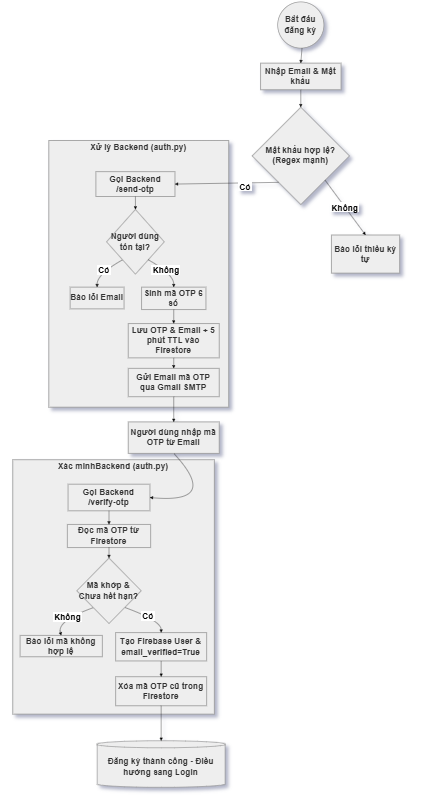
\includegraphics[height=0.74\textheight,keepaspectratio]{tai_nguyen/media/image22.png}
\caption{Lưu đồ thuật toán đăng ký và xác thực OTP}
\label{fig:3-16}
\end{figure}

\begin{figure}[H]
\centering
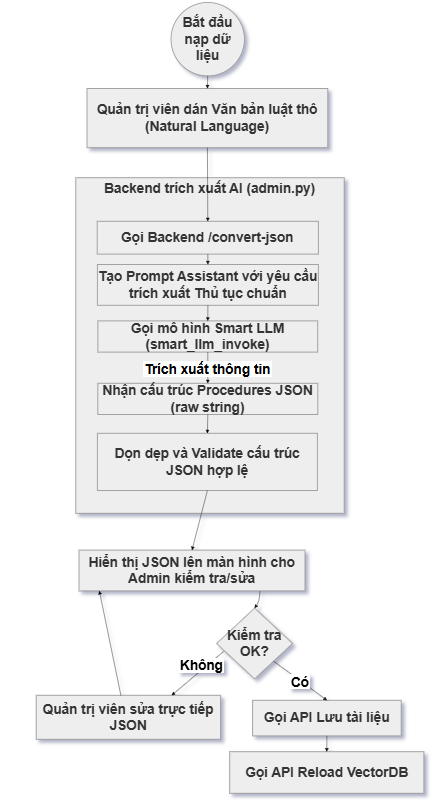
\includegraphics[height=0.74\textheight,keepaspectratio]{tai_nguyen/media/image23.png}
\caption{Lưu đồ trích xuất JSON bằng AI cho quản trị viên}
\label{fig:3-17}
\end{figure}

\begin{figure}[H]
\centering
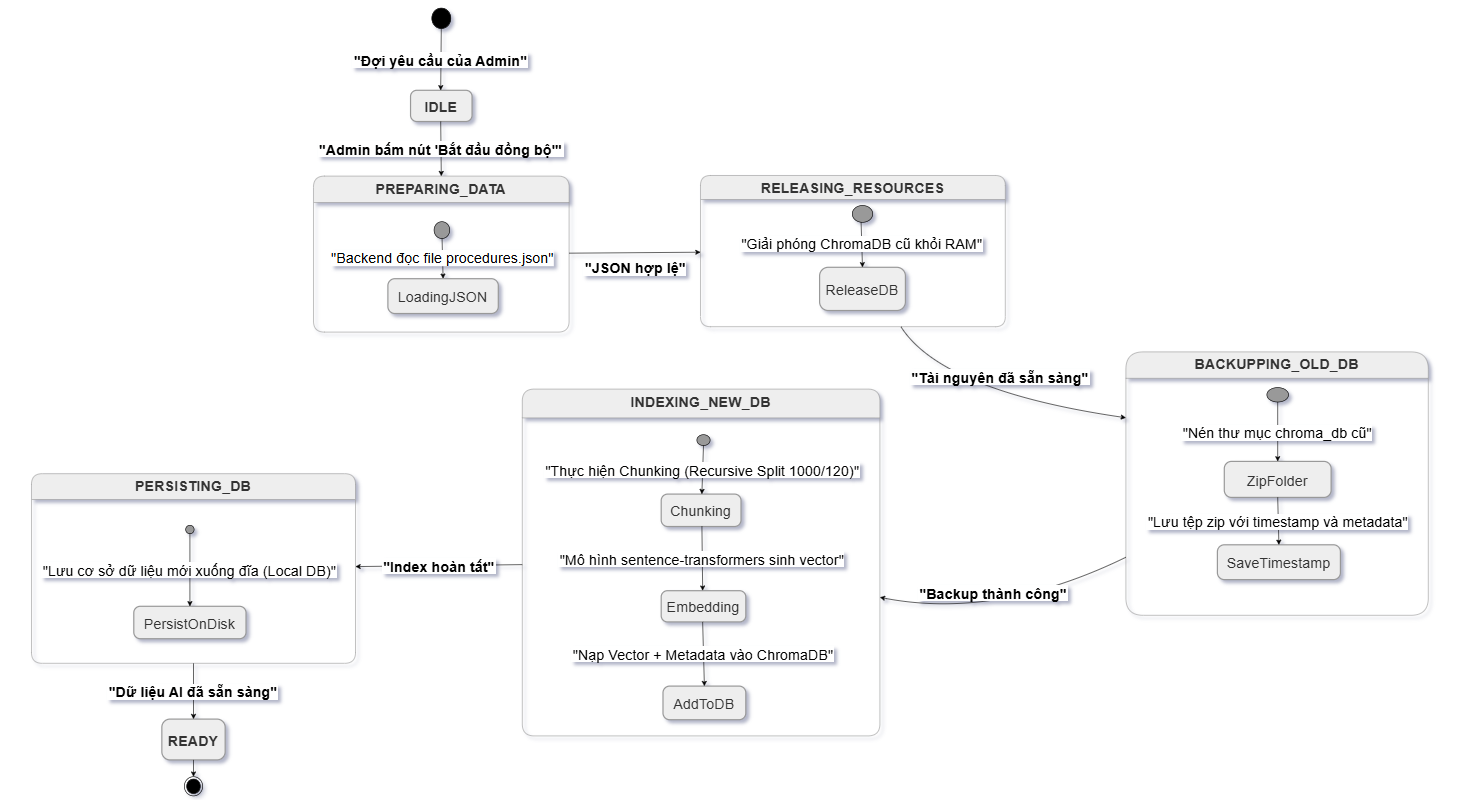
\includegraphics[width=0.92\textwidth]{tai_nguyen/media/image24.png}
\caption{Biểu đồ trạng thái đồng bộ và sao lưu VectorDB}
\label{fig:3-18}
\end{figure}


\clearpage
\mychapter{4}{CHƯƠNG 4: TRIỂN KHAI}
\addcontentsline{toc}{chapter}{CHƯƠNG 4: TRIỂN KHAI}
Chương này trình bày quá trình hiện thực hóa hệ thống chatbot hỗ trợ tra
cứu TTHC cho tỉnh Lai Châu sau giai đoạn phân tích và thiết kế. Nội dung
chương được tổ chức theo trình tự triển khai thực tế: cài đặt backend,
cài đặt frontend, bảo vệ hệ thống, quản trị kho tri thức, kiểm thử chức
năng, đánh giá chatbot RAG và hướng dẫn sử dụng.

Trọng tâm của chương không chỉ là mô tả cách chạy hệ thống mà còn thể
hiện minh chứng vận hành và kết quả đánh giá trên bộ 100 câu hỏi thử
nghiệm. Các kết quả đánh giá được ghi nhận từ file chạy test API, gồm
câu hỏi, câu trả lời thực tế, thời gian phản hồi và nhận xét đối chiếu
với dữ liệu nguồn.

\section{Cài đặt backend và pipeline
RAG}

Backend là thành phần trung tâm của hệ thống. Mọi luồng quan trọng đều
đi qua backend: nhận câu hỏi, kiểm tra đăng nhập, lấy lịch sử hội thoại,
chạy pipeline RAG, gọi mô hình ngôn ngữ, lưu kết quả và xử lý chức năng
quản trị. Quá trình cài đặt backend gồm tạo môi trường ảo Python, cài
thư viện từ requirements.txt, cấu hình .env, đặt serviceAccountKey.json
ở phía backend và chuẩn bị thư mục data chứa procedures.json,
entities.json, synonyms.json, intents.json và all\_laichau\_codes.json.

\section{Cài đặt frontend và kết nối
API}

Frontend là phần người dùng trực tiếp thao tác. Giao diện được tổ chức
theo các component chính như LoginPage, ChatBox, Sidebar, InputBox,
Message và AdminDashboard. Cách chia component giúp quá trình phát
triển, kiểm thử và mở rộng giao diện thuận lợi hơn.

\begin{longtable}[]{|
  >{\raggedright\arraybackslash}p{(\columnwidth - 4\tabcolsep) * \real{0.1651}}|
  >{\raggedright\arraybackslash}p{(\columnwidth - 4\tabcolsep) * \real{0.2568}}|
  >{\raggedright\arraybackslash}p{(\columnwidth - 4\tabcolsep) * \real{0.5781}}|}
\caption{API chính frontend sử dụng}\\
\hline
\begin{minipage}[b]{\linewidth}\raggedright
\textbf{Nhóm}
\end{minipage} & \begin{minipage}[b]{\linewidth}\raggedright
\textbf{Endpoint}
\end{minipage} & \begin{minipage}[b]{\linewidth}\raggedright
\textbf{Mục đích}
\end{minipage} \\
\hline
\endfirsthead
\continuedcaption{API chính frontend sử dụng}
\hline
\begin{minipage}[b]{\linewidth}\raggedright
\textbf{Nhóm}
\end{minipage} & \begin{minipage}[b]{\linewidth}\raggedright
\textbf{Endpoint}
\end{minipage} & \begin{minipage}[b]{\linewidth}\raggedright
\textbf{Mục đích}
\end{minipage} \\
\hline
\endhead
\hline
\endlastfoot
Auth & /auth/send-otp & Gửi mã OTP khi người dùng đăng ký bằng email. \\
\hline
Auth & /auth/verify-otp & Xác minh OTP và hoàn tất tạo tài khoản. \\
\hline
Auth & /auth/check-admin & Kiểm tra tài khoản hiện tại có quyền admin
hay không. \\
\hline
User & /user/chat & Gửi câu hỏi đến chatbot và nhận câu trả lời. \\
\hline
User & /user/sessions & Lấy danh sách phiên hội thoại. \\
\hline
User & /user/chat/history & Lấy lại tin nhắn trong một phiên chat. \\
\hline
Admin & /admin/stats & Lấy số liệu thống kê và dữ liệu biểu đồ. \\
\hline
Admin & /admin/documents & Quản lý dữ liệu thủ tục hành chính. \\
\hline
Admin & /admin/convert-json & Dùng AI trích xuất văn bản thô thành
JSON. \\
\hline
Admin & /admin/reload-vectordb & Đồng bộ lại ChromaDB sau khi dữ liệu
thay đổi. \\
\hline
Admin & /admin/backups & Liệt kê hoặc xóa bản sao lưu VectorDB. \\
\hline
\end{longtable}

\emph{Backend được khởi chạy bằng Uvicorn, frontend được chạy bằng Vite
và backend có thể mở ra môi trường thử nghiệm bằng ngrok (xem các lệnh
chạy hệ thống tại Phụ lục B).}

\section{Bảo vệ hệ thống và dữ
liệu}

Hệ thống lưu lịch sử hội thoại và có khu vực quản trị, vì vậy cơ chế bảo
vệ phải được đặt ở backend. Mọi request cần bảo vệ đều sử dụng Firebase
ID Token và được backend xác minh trước khi xử lý. Các chức năng quản
trị tiếp tục kiểm tra email admin để tránh người dùng thường gọi trực
tiếp API quản trị.

\begin{figure}[H]
\centering
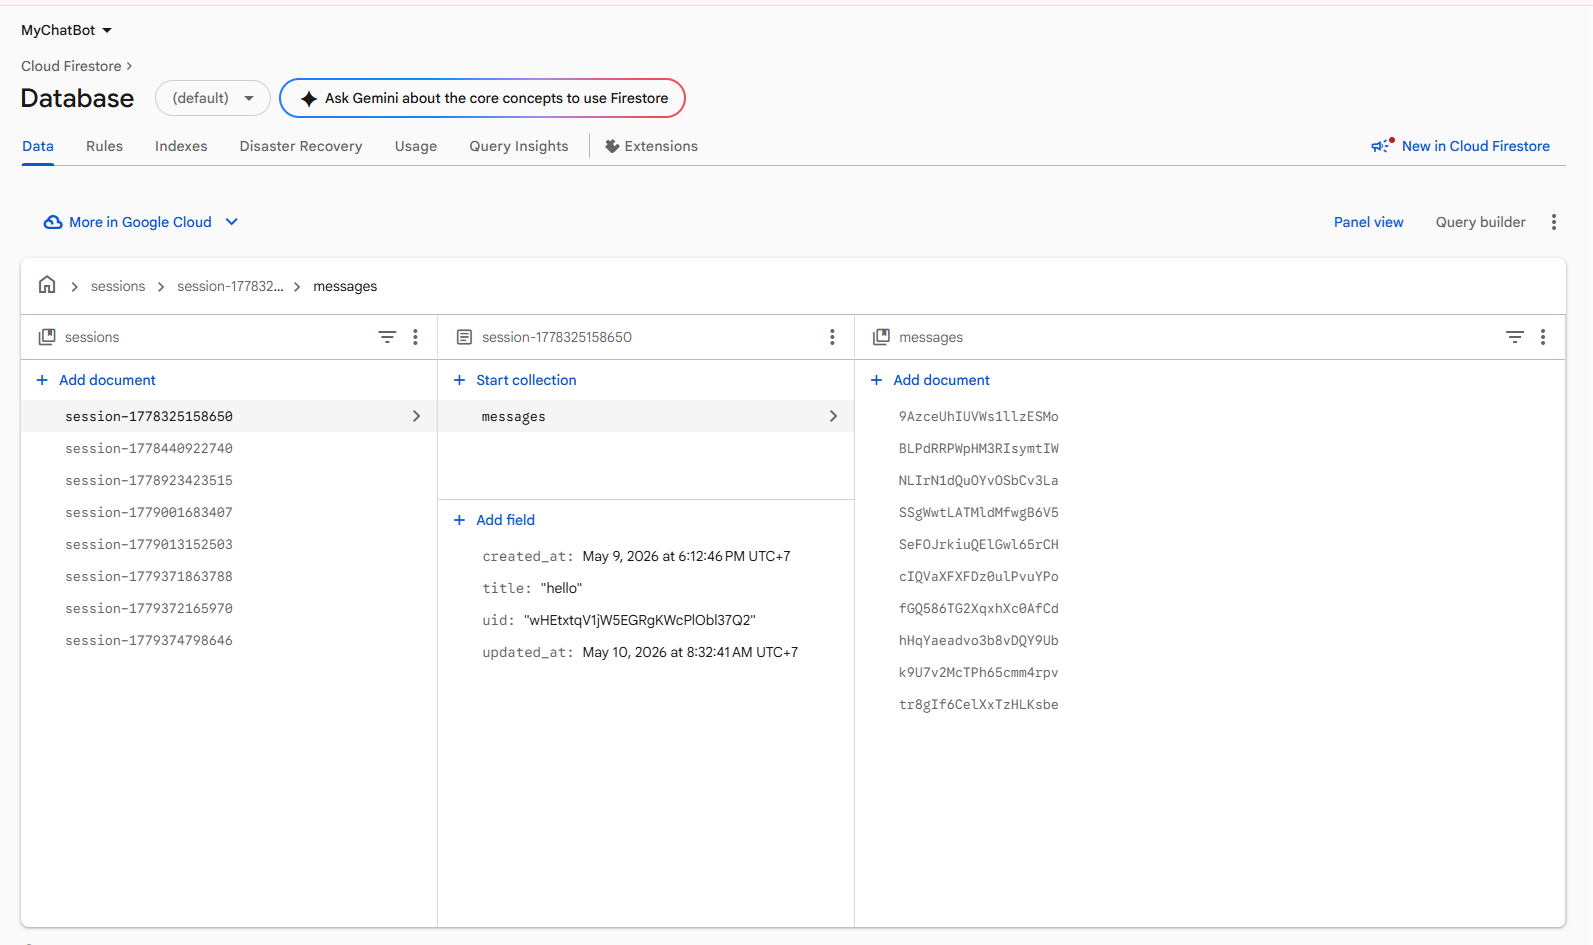
\includegraphics[width=0.92\textwidth]{tai_nguyen/media/image25.png}
\caption{Minh chứng Firestore lưu phiên hội thoại và tin nhắn}
\label{fig:4-1}
\end{figure}

\begin{longtable}[]{|
  >{\raggedright\arraybackslash}p{(\columnwidth - 4\tabcolsep) * \real{0.1823}}|
  >{\raggedright\arraybackslash}p{(\columnwidth - 4\tabcolsep) * \real{0.4415}}|
  >{\raggedright\arraybackslash}p{(\columnwidth - 4\tabcolsep) * \real{0.3762}}|}
\caption{Checklist bảo vệ khi triển khai}\\
\hline
\begin{minipage}[b]{\linewidth}\raggedright
\textbf{Hạng mục}
\end{minipage} & \begin{minipage}[b]{\linewidth}\raggedright
\textbf{Cách triển khai}
\end{minipage} & \begin{minipage}[b]{\linewidth}\raggedright
\textbf{Mục đích}
\end{minipage} \\
\hline
\endfirsthead
\continuedcaption{Checklist bảo vệ khi triển khai}
\hline
\begin{minipage}[b]{\linewidth}\raggedright
\textbf{Hạng mục}
\end{minipage} & \begin{minipage}[b]{\linewidth}\raggedright
\textbf{Cách triển khai}
\end{minipage} & \begin{minipage}[b]{\linewidth}\raggedright
\textbf{Mục đích}
\end{minipage} \\
\hline
\endhead
\hline
\endlastfoot
Token người dùng & Verify Firebase ID Token ở backend & Tránh giả mạo
đăng nhập. \\
\hline
Quyền admin & Kiểm tra email admin trước khi chạy API quản trị & Ngăn
người dùng thường sửa dữ liệu hoặc reload VectorDB. \\
\hline
OTP đăng ký & Lưu OTP có thời hạn và xác minh trước khi tạo tài khoản &
Giảm tài khoản ảo và kiểm tra quyền sở hữu email. \\
\hline
Khóa dịch vụ & Đặt API key và service account ở backend/secret & Tránh
lộ khóa khi nộp mã nguồn hoặc deploy frontend. \\
\hline
Dữ liệu hội thoại & Lưu theo uid/session\_id và giới hạn lịch sử đưa vào
prompt & Giảm rủi ro lộ dữ liệu cá nhân. \\
\hline
VectorDB & Backup trước khi reload và dọn backup quá hạn & Có điểm khôi
phục khi build dữ liệu lỗi. \\
\hline
\end{longtable}

\section{Hoạt động thử nghiệm, kiểm thử và
đánh giá định
lượng}

Kiểm thử hệ thống RAG cần bao phủ cả phần mềm truyền thống và chất lượng
AI. Với phần mềm truyền thống, các luồng xác thực, lưu lịch sử, phân
quyền admin, quản lý dữ liệu và reload VectorDB được kiểm thử bằng kịch
bản đầu vào - kết quả mong đợi. Với chatbot RAG, quá trình đánh giá sử
dụng bộ 100 câu hỏi để xem xét độ đúng của câu trả lời, khả năng từ chối
ngoài phạm vi và thời gian phản hồi.

\begin{longtable}[]{|
  >{\raggedright\arraybackslash}p{(\columnwidth - 10\tabcolsep) * \real{0.1467}}|
  >{\raggedright\arraybackslash}p{(\columnwidth - 10\tabcolsep) * \real{0.1282}}|
  >{\raggedright\arraybackslash}p{(\columnwidth - 10\tabcolsep) * \real{0.1995}}|
  >{\raggedright\arraybackslash}p{(\columnwidth - 10\tabcolsep) * \real{0.2105}}|
  >{\raggedright\arraybackslash}p{(\columnwidth - 10\tabcolsep) * \real{0.2146}}|
  >{\raggedright\arraybackslash}p{(\columnwidth - 10\tabcolsep) * \real{0.1004}}|}
\caption{Kịch bản kiểm thử chức năng có minh chứng}\\
\hline
\begin{minipage}[b]{\linewidth}\raggedright
\textbf{Mã ca}
\end{minipage} & \begin{minipage}[b]{\linewidth}\raggedright
\textbf{Kịch bản}
\end{minipage} & \begin{minipage}[b]{\linewidth}\raggedright
\textbf{Dữ liệu đầu vào}
\end{minipage} & \begin{minipage}[b]{\linewidth}\raggedright
\textbf{Kết quả mong đợi}
\end{minipage} & \begin{minipage}[b]{\linewidth}\raggedright
\textbf{Minh chứng}
\end{minipage} & \begin{minipage}[b]{\linewidth}\raggedright
\textbf{Trạng thái}
\end{minipage} \\
\hline
\endfirsthead
\continuedcaption{Kịch bản kiểm thử chức năng có minh chứng}
\hline
\begin{minipage}[b]{\linewidth}\raggedright
\textbf{Mã ca}
\end{minipage} & \begin{minipage}[b]{\linewidth}\raggedright
\textbf{Kịch bản}
\end{minipage} & \begin{minipage}[b]{\linewidth}\raggedright
\textbf{Dữ liệu đầu vào}
\end{minipage} & \begin{minipage}[b]{\linewidth}\raggedright
\textbf{Kết quả mong đợi}
\end{minipage} & \begin{minipage}[b]{\linewidth}\raggedright
\textbf{Minh chứng}
\end{minipage} & \begin{minipage}[b]{\linewidth}\raggedright
\textbf{Trạng thái}
\end{minipage} \\
\hline
\endhead
\hline
\endlastfoot
AUTH\_01 & Đăng ký email mới và sinh OTP & Email hợp lệ, mật khẩu hợp lệ
& Sinh OTP, lưu tạm trong Firestore và cho phép xác minh tài khoản. &
Ảnh Firebase Auth/Firestore, màn hình OTP & Đạt \\
\hline
AUTH\_02 & Truy cập API không có token & Không gửi Authorization header
& Backend từ chối request bằng lỗi xác thực. & Response API hoặc
Swagger/log backend & Đạt \\
\hline
CHAT\_01 & Hỏi hồ sơ thủ tục cụ thể & Giải quyết chế độ mai táng phí đối
với cựu chiến binh cần giấy tờ gì? & Chatbot trả lời theo thành phần hồ
sơ từ dữ liệu nguồn. & Ảnh màn hình chatbot và dòng kết quả trong CSV &
Đạt \\
\hline
CHAT\_02 & Câu hỏi tiếp nối & Ngữ cảnh trước + câu hỏi: Thế lệ phí bao
nhiêu? & Chatbot dùng lịch sử để hiểu thủ tục đang hỏi. & Kết quả TC 081
trong file test & Đạt \\
\hline
CHAT\_03 & Câu hỏi ngoài phạm vi & Dự đoán giá vàng hoặc kết quả xổ số &
Chatbot từ chối, không tự bịa thủ tục. & Kết quả TC 096-TC\_100 & Đạt \\
\hline
ADM\_01 & Xem thống kê hệ thống & Tài khoản admin hợp lệ & Dashboard
hiển thị số liệu và biểu đồ. & Ảnh trang thống kê admin & Đạt \\
\hline
ADM\_02 & Quản lý dữ liệu thủ tục & JSON thủ tục hợp lệ & Dữ liệu được
cập nhật và có thể reload VectorDB. & Ảnh quản lý dữ liệu và reload
VectorDB & Đạt \\
\hline
\end{longtable}

\begin{longtable}[]{|
  >{\raggedright\arraybackslash}p{(\columnwidth - 2\tabcolsep) * \real{0.5007}}|
  >{\raggedright\arraybackslash}p{(\columnwidth - 2\tabcolsep) * \real{0.4993}}|}
\caption{Phân nhóm bộ 100 câu hỏi thử nghiệm chatbot RAG}\\
\hline
\begin{minipage}[b]{\linewidth}\raggedright
\textbf{Nhóm}
\end{minipage} & \begin{minipage}[b]{\linewidth}\raggedright
\textbf{Số lượng}
\end{minipage} \\
\hline
\endfirsthead
\continuedcaption{Phân nhóm bộ 100 câu hỏi thử nghiệm chatbot RAG}
\hline
\begin{minipage}[b]{\linewidth}\raggedright
\textbf{Nhóm}
\end{minipage} & \begin{minipage}[b]{\linewidth}\raggedright
\textbf{Số lượng}
\end{minipage} \\
\hline
\endhead
\hline
\endlastfoot
Thành phần hồ sơ & 15 \\
\hline
Thời hạn giải quyết & 15 \\
\hline
Phí/lệ phí & 15 \\
\hline
Cơ quan thực hiện & 10 \\
\hline
Cách thức thực hiện & 10 \\
\hline
Căn cứ pháp lý & 10 \\
\hline
Kết quả thực hiện & 5 \\
\hline
Hội thoại tiếp nối & 5 \\
\hline
Câu hỏi bẫy/gây nhiễu & 10 \\
\hline
Ngoài phạm vi & 5 \\
\hline
\end{longtable}

\emph{Bảng 4.4 cho biết cách phân bố 100 câu hỏi theo từng nhóm nội dung
đánh giá. Danh sách đầy đủ 100 câu hỏi kiểm thử, kết quả đánh giá, thời
gian phản hồi và điểm hiệu năng của từng test được trình bày tại Phụ lục
D.}

\begin{figure}[H]
\centering
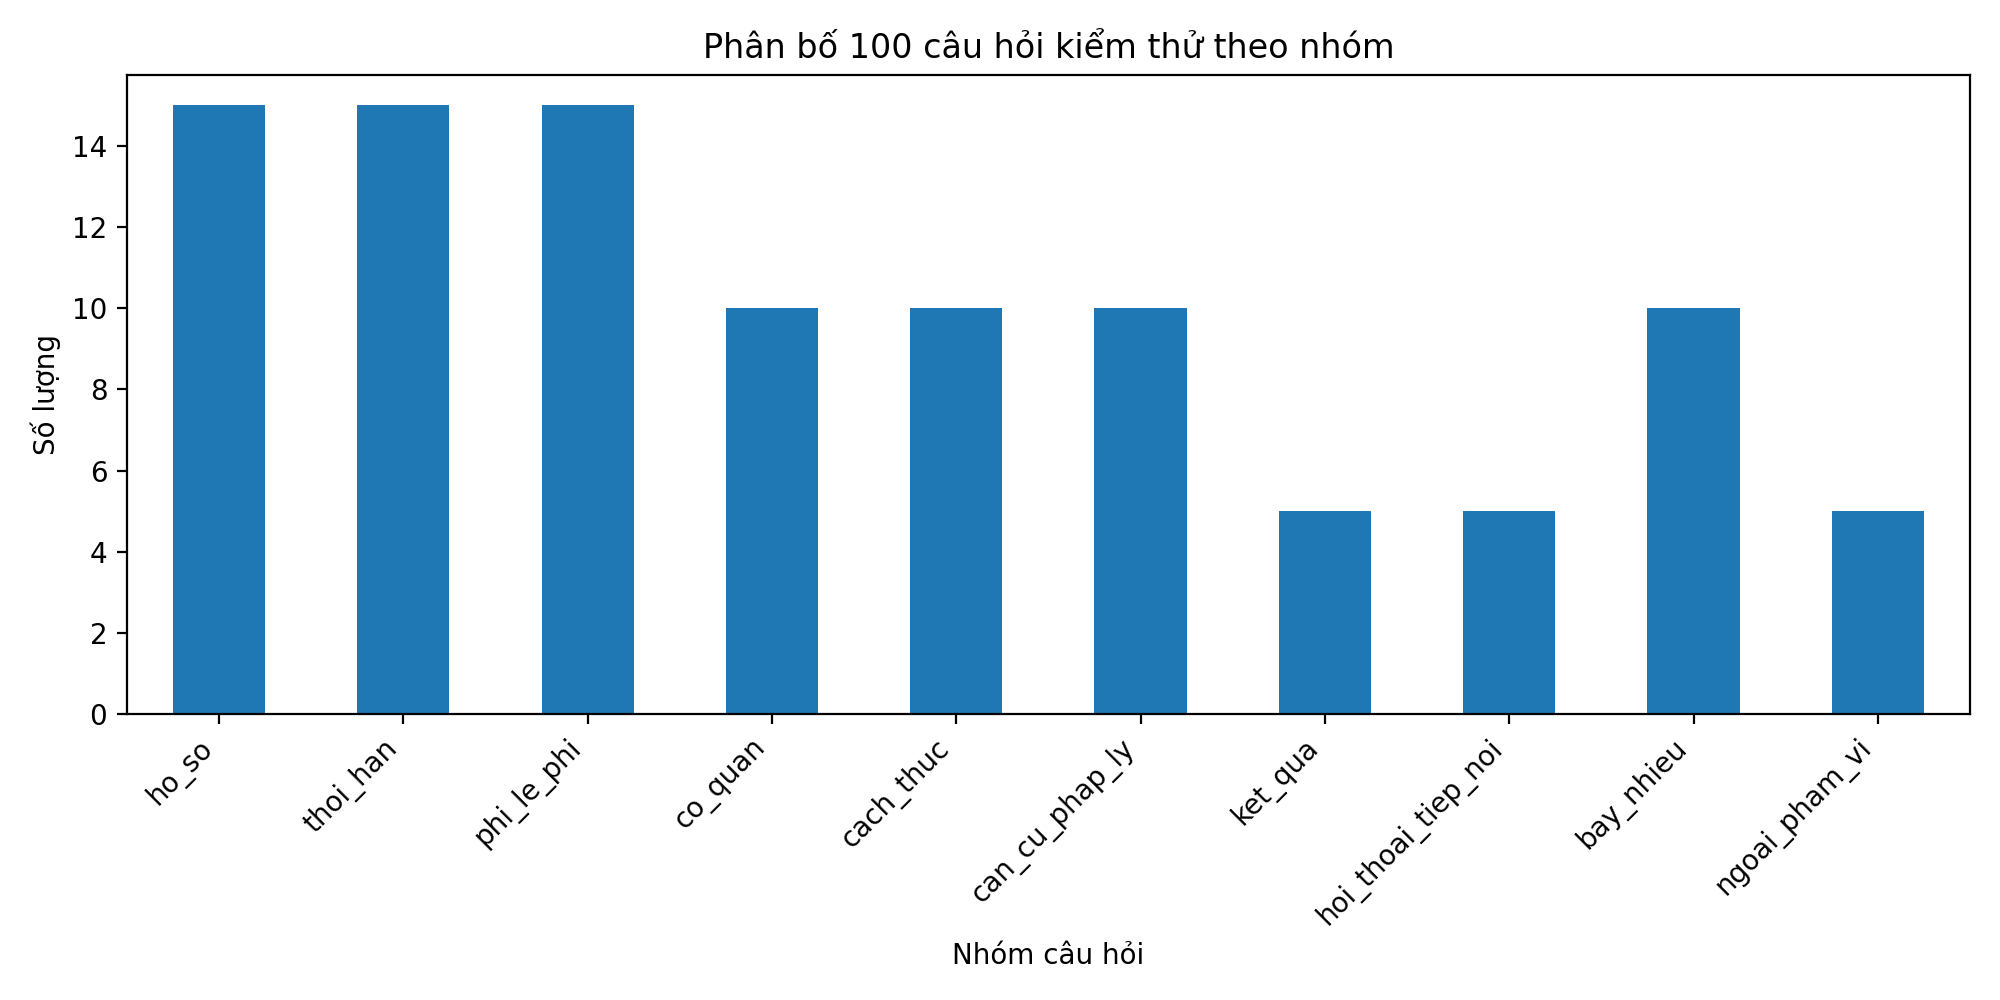
\includegraphics[width=0.92\textwidth]{tai_nguyen/media/image26.png}
\caption{Biểu đồ phân bố 100 câu hỏi kiểm thử theo nhóm}
\label{fig:4-2}
\end{figure}

\begin{longtable}[]{|
  >{\raggedright\arraybackslash}p{(\columnwidth - 4\tabcolsep) * \real{0.2561}}|
  >{\raggedright\arraybackslash}p{(\columnwidth - 4\tabcolsep) * \real{0.1852}}|
  >{\raggedright\arraybackslash}p{(\columnwidth - 4\tabcolsep) * \real{0.5587}}|}
\caption{Kết quả đánh giá định lượng chatbot RAG}\\
\hline
\begin{minipage}[b]{\linewidth}\raggedright
\textbf{Chỉ số}
\end{minipage} & \begin{minipage}[b]{\linewidth}\raggedright
\textbf{Kết quả ghi nhận}
\end{minipage} & \begin{minipage}[b]{\linewidth}\raggedright
\textbf{Nhận xét}
\end{minipage} \\
\hline
\endfirsthead
\continuedcaption{Kết quả đánh giá định lượng chatbot RAG}
\hline
\begin{minipage}[b]{\linewidth}\raggedright
\textbf{Chỉ số}
\end{minipage} & \begin{minipage}[b]{\linewidth}\raggedright
\textbf{Kết quả ghi nhận}
\end{minipage} & \begin{minipage}[b]{\linewidth}\raggedright
\textbf{Nhận xét}
\end{minipage} \\
\hline
\endhead
\hline
\endlastfoot
Số câu hỏi kiểm thử & 100 câu & Bộ test được sinh từ dữ liệu
procedures.json. \\
\hline
Câu trả lời đúng & 82/100 (82.0\%) & Chỉ tính các câu trả lời đúng hoặc
từ chối đúng. \\
\hline
Câu trả lời chấp nhận được & 92/100 (92.0\%) & Gồm đúng, đúng nhưng
thiếu ý và từ chối đúng. \\
\hline
Từ chối đúng ngoài phạm vi & 5/5 (100.0\%) & Áp dụng cho nhóm câu hỏi
ngoài phạm vi. \\
\hline
Latency trung bình & 16.49 giây & Đo từ lúc gửi request đến khi nhận
response. \\
\hline
Latency nhỏ nhất & 6.63 giây & Ghi nhận trong file kết quả test. \\
\hline
Latency lớn nhất & 51.33 giây & Truy vấn chậm nhất trong bộ 100 câu. \\
\hline
Latency P95 & 34.79 giây & 95\% số câu có thời gian phản hồi không vượt
quá giá trị này. \\
\hline
Top-k retrieval accuracy & Chưa đo trực tiếp & API hiện chưa trả danh
sách chunk/sources hoặc log top-k nên chưa tính chính xác từ file kết
quả hiện có. \\
\hline
\end{longtable}

\begin{figure}[H]
\centering
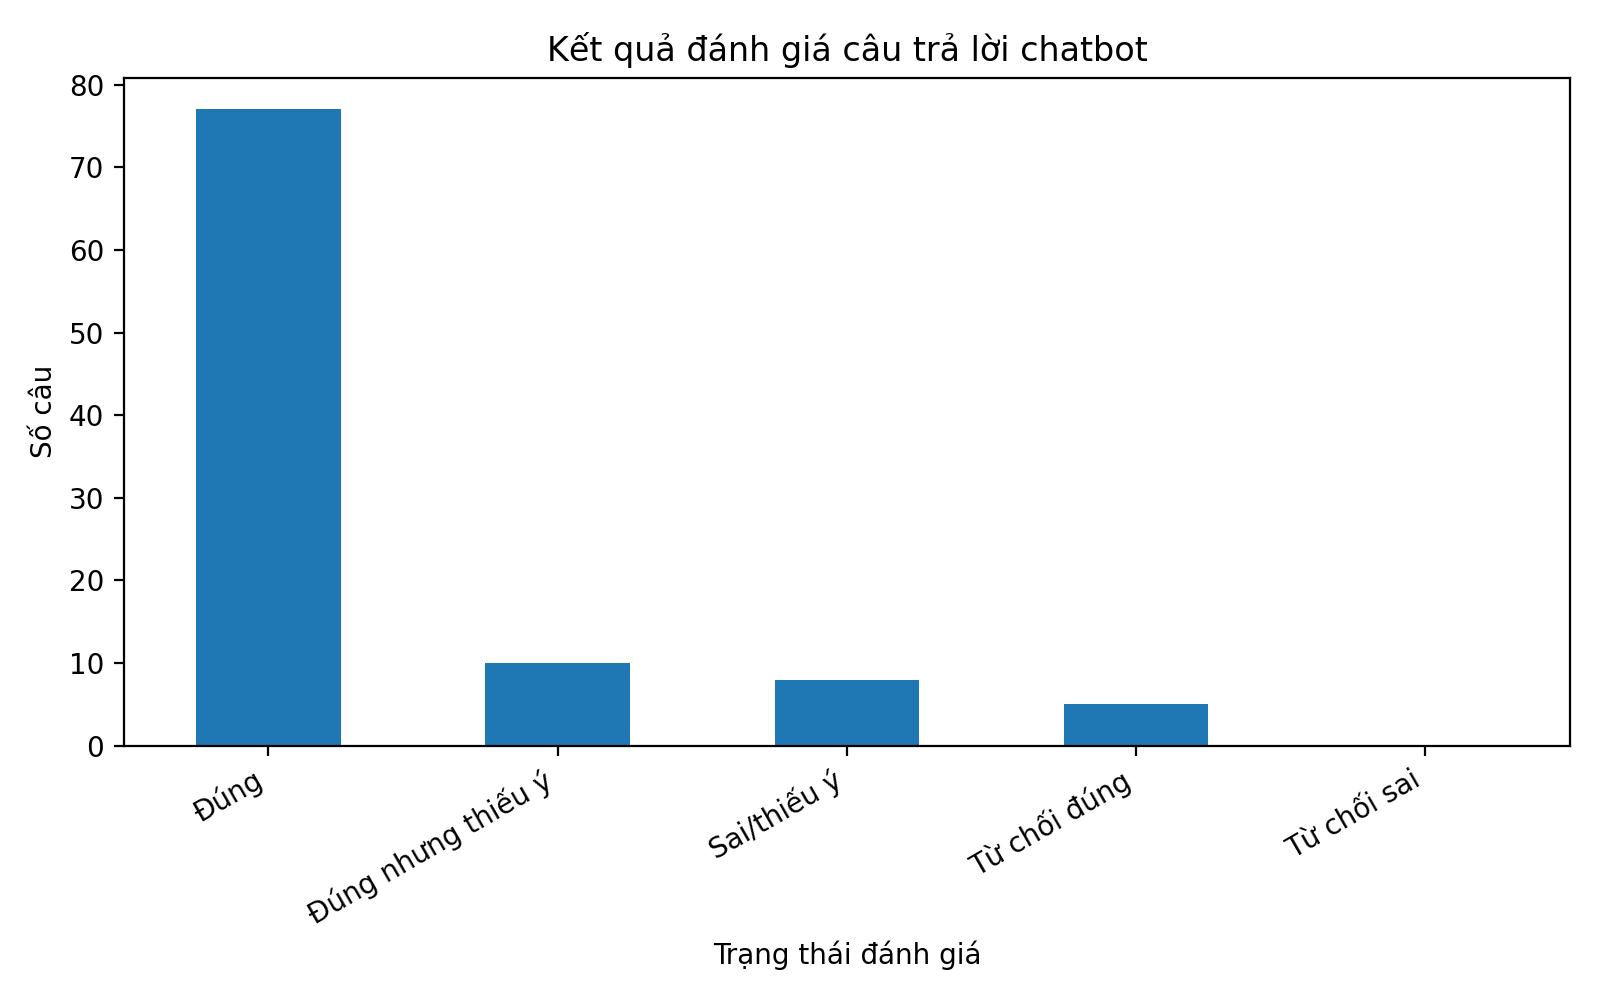
\includegraphics[width=0.92\textwidth]{tai_nguyen/media/image27.png}
\caption{Kết quả đánh giá câu trả lời chatbot}
\label{fig:4-3}
\end{figure}

\begin{figure}[H]
\centering
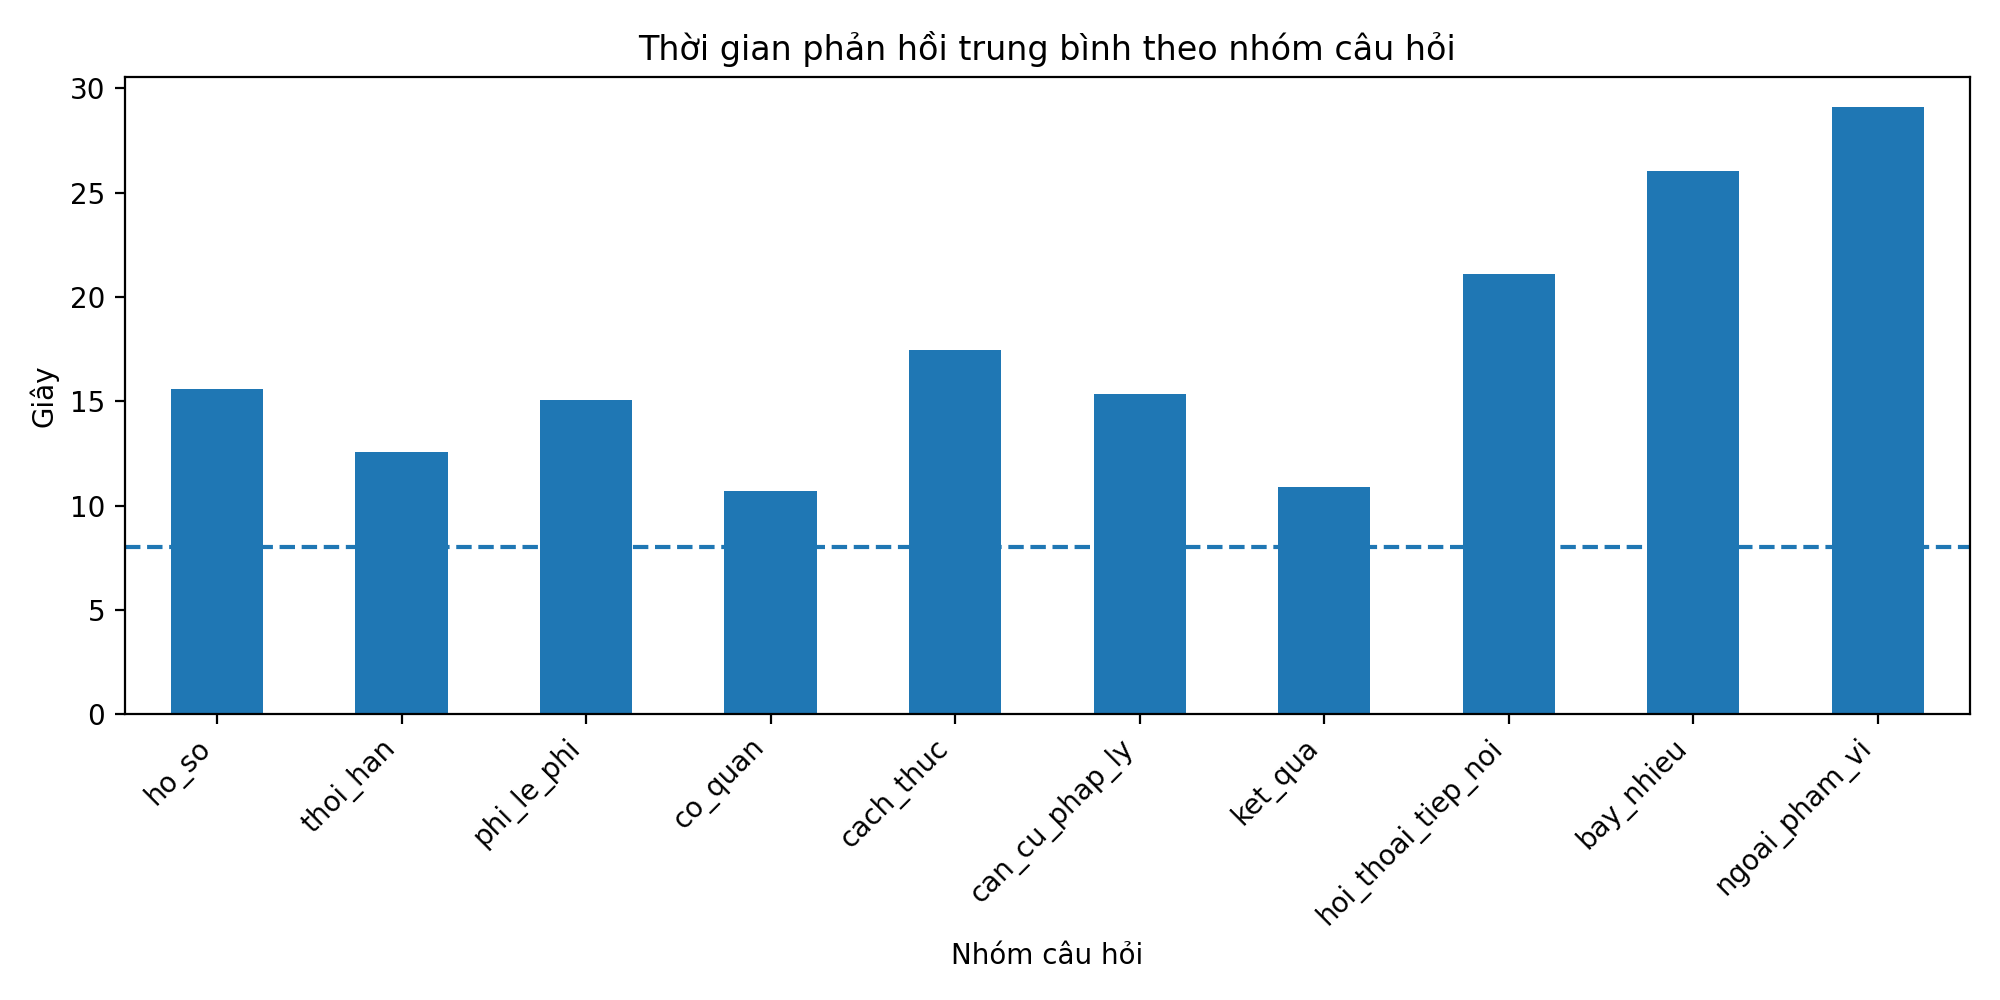
\includegraphics[width=0.92\textwidth]{tai_nguyen/media/image28.png}
\caption{Thời gian phản hồi trung bình theo nhóm câu hỏi}
\label{fig:4-4}
\end{figure}

\begin{longtable}[]{|
  >{\raggedright\arraybackslash}p{(\columnwidth - 10\tabcolsep) * \real{0.2242}}|
  >{\raggedright\arraybackslash}p{(\columnwidth - 10\tabcolsep) * \real{0.0936}}|
  >{\raggedright\arraybackslash}p{(\columnwidth - 10\tabcolsep) * \real{0.2122}}|
  >{\raggedright\arraybackslash}p{(\columnwidth - 10\tabcolsep) * \real{0.1403}}|
  >{\raggedright\arraybackslash}p{(\columnwidth - 10\tabcolsep) * \real{0.1670}}|
  >{\raggedright\arraybackslash}p{(\columnwidth - 10\tabcolsep) * \real{0.1628}}|}
\caption{Tổng hợp trạng thái đánh giá theo nhóm câu hỏi}\\
\hline
\begin{minipage}[b]{\linewidth}\raggedright
\textbf{Nhóm}
\end{minipage} & \begin{minipage}[b]{\linewidth}\raggedright
\textbf{Đúng}
\end{minipage} & \begin{minipage}[b]{\linewidth}\raggedright
\textbf{Đúng nhưng thiếu ý}
\end{minipage} & \begin{minipage}[b]{\linewidth}\raggedright
\textbf{Sai/thiếu ý}
\end{minipage} & \begin{minipage}[b]{\linewidth}\raggedright
\textbf{Từ chối đúng}
\end{minipage} & \begin{minipage}[b]{\linewidth}\raggedright
\textbf{Từ chối sai}
\end{minipage} \\
\hline
\endfirsthead
\continuedcaption{Tổng hợp trạng thái đánh giá theo nhóm câu hỏi}
\hline
\begin{minipage}[b]{\linewidth}\raggedright
\textbf{Nhóm}
\end{minipage} & \begin{minipage}[b]{\linewidth}\raggedright
\textbf{Đúng}
\end{minipage} & \begin{minipage}[b]{\linewidth}\raggedright
\textbf{Đúng nhưng thiếu ý}
\end{minipage} & \begin{minipage}[b]{\linewidth}\raggedright
\textbf{Sai/thiếu ý}
\end{minipage} & \begin{minipage}[b]{\linewidth}\raggedright
\textbf{Từ chối đúng}
\end{minipage} & \begin{minipage}[b]{\linewidth}\raggedright
\textbf{Từ chối sai}
\end{minipage} \\
\hline
\endhead
\hline
\endlastfoot
Câu hỏi bẫy/gây nhiễu & 5 & 1 & 4 & 0 & 0 \\
\hline
Cách thức thực hiện & 10 & 0 & 0 & 0 & 0 \\
\hline
Căn cứ pháp lý & 8 & 1 & 1 & 0 & 0 \\
\hline
Cơ quan thực hiện & 9 & 0 & 1 & 0 & 0 \\
\hline
Thành phần hồ sơ & 10 & 4 & 1 & 0 & 0 \\
\hline
Hội thoại tiếp nối & 4 & 1 & 0 & 0 & 0 \\
\hline
Kết quả thực hiện & 5 & 0 & 0 & 0 & 0 \\
\hline
Ngoài phạm vi & 0 & 0 & 0 & 5 & 0 \\
\hline
Phí/lệ phí & 15 & 0 & 0 & 0 & 0 \\
\hline
Thời hạn giải quyết & 11 & 3 & 1 & 0 & 0 \\
\hline
\end{longtable}

\begin{longtable}[]{|
  >{\raggedright\arraybackslash}p{(\columnwidth - 4\tabcolsep) * \real{0.3478}}|
  >{\raggedright\arraybackslash}p{(\columnwidth - 4\tabcolsep) * \real{0.1366}}|
  >{\raggedright\arraybackslash}p{(\columnwidth - 4\tabcolsep) * \real{0.5156}}|}
\caption{So sánh kết quả với baseline tìm kiếm từ khóa mô phỏng}\\
\hline
\begin{minipage}[b]{\linewidth}\raggedright
\textbf{Phương án/chỉ số}
\end{minipage} & \begin{minipage}[b]{\linewidth}\raggedright
\textbf{Kết quả}
\end{minipage} & \begin{minipage}[b]{\linewidth}\raggedright
\textbf{Ghi chú}
\end{minipage} \\
\hline
\endfirsthead
\continuedcaption{So sánh kết quả với baseline tìm kiếm từ khóa mô phỏng}
\hline
\begin{minipage}[b]{\linewidth}\raggedright
\textbf{Phương án/chỉ số}
\end{minipage} & \begin{minipage}[b]{\linewidth}\raggedright
\textbf{Kết quả}
\end{minipage} & \begin{minipage}[b]{\linewidth}\raggedright
\textbf{Ghi chú}
\end{minipage} \\
\hline
\endhead
\hline
\endlastfoot
Tìm kiếm từ khóa mô phỏng - Top 1 & 24.2\% & Tính bằng trùng khớp từ
khóa trên tên/nội dung thủ tục. \\
\hline
Tìm kiếm từ khóa mô phỏng - Top 3 & 42.1\% & Kiểm tra thủ tục kỳ vọng có
nằm trong 3 kết quả đầu. \\
\hline
Tìm kiếm từ khóa mô phỏng - Top 5 & 53.7\% & Kiểm tra thủ tục kỳ vọng có
nằm trong 5 kết quả đầu. \\
\hline
Chatbot RAG - trả lời đúng & 82.0\% & Đánh giá theo câu trả lời thực tế
của hệ thống. \\
\hline
Chatbot RAG - chấp nhận được & 92.0\% & Tính cả các câu đúng nhưng thiếu
ý. \\
\hline
\end{longtable}

\begin{figure}[H]
\centering
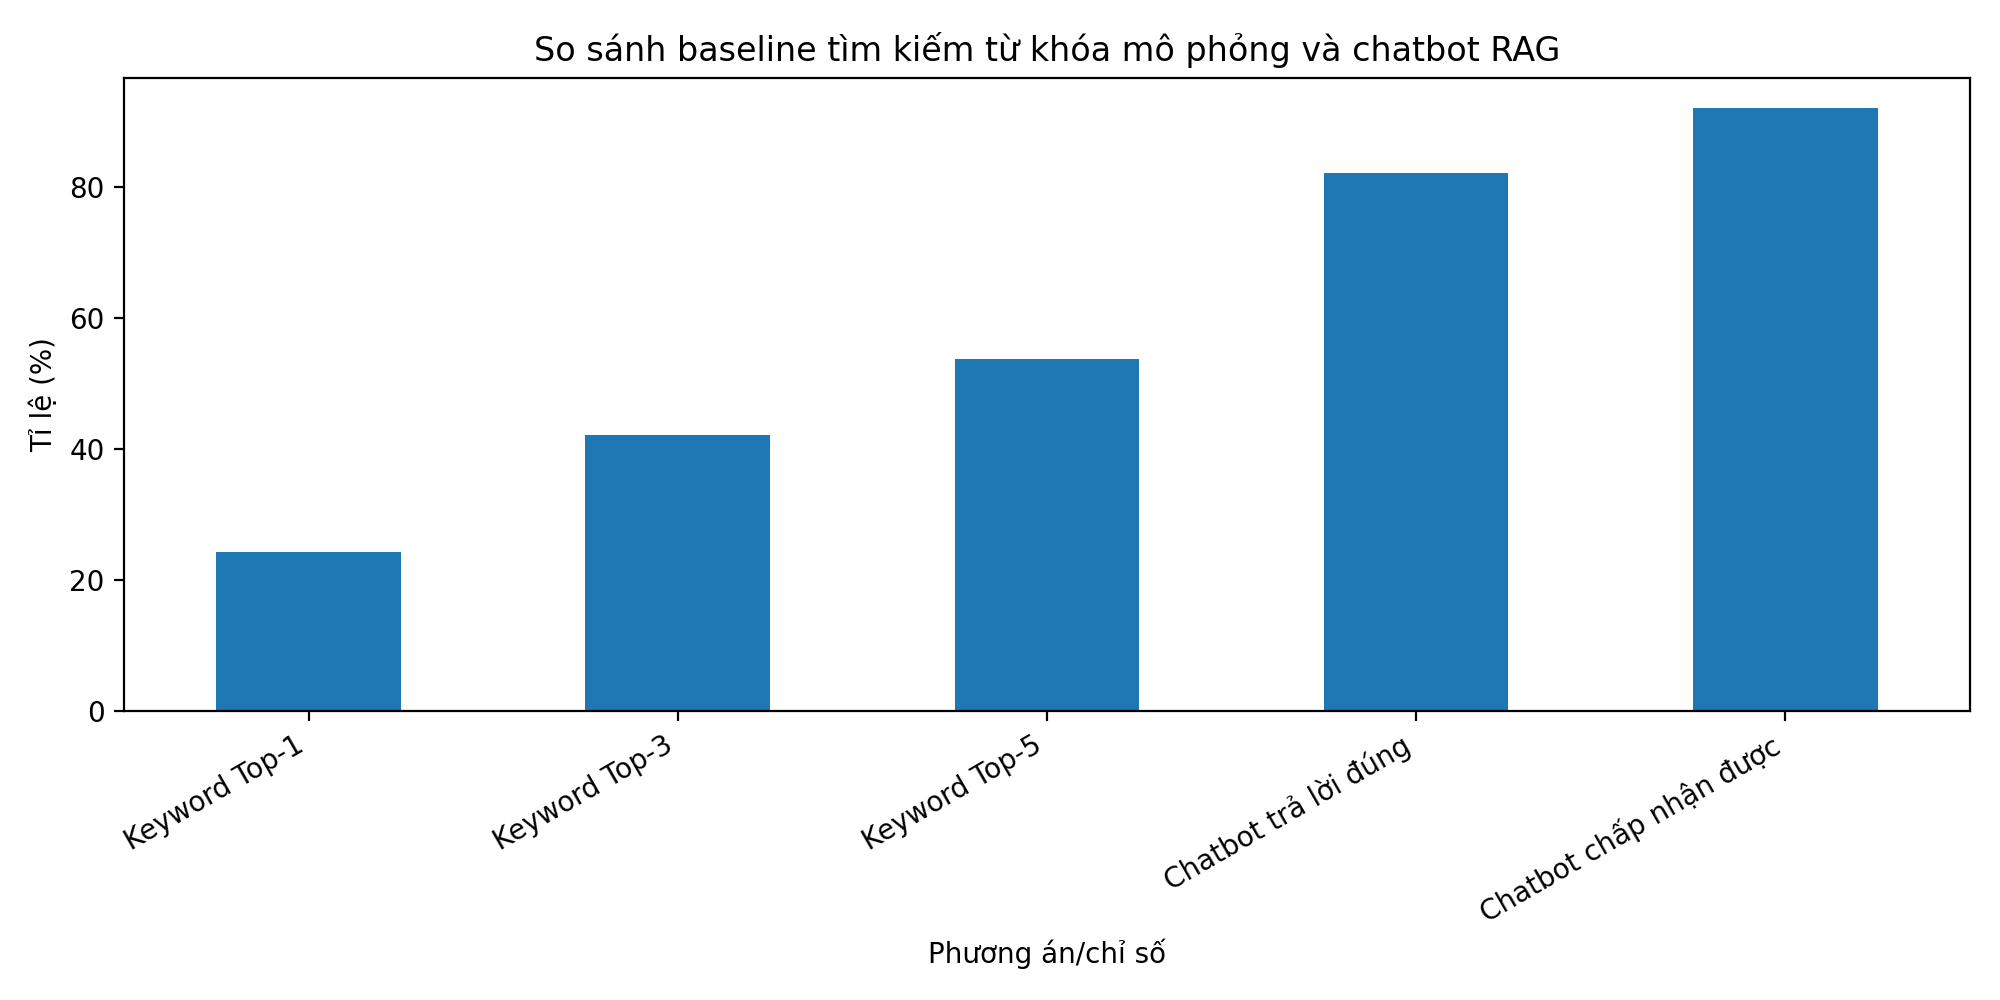
\includegraphics[width=0.92\textwidth]{tai_nguyen/media/image29.png}
\caption{So sánh baseline tìm kiếm từ khóa mô phỏng và chatbot RAG}
\label{fig:4-5}
\end{figure}

\begin{longtable}[]{|
  >{\raggedright\arraybackslash}p{(\columnwidth - 10\tabcolsep) * \real{0.0777}}|
  >{\raggedright\arraybackslash}p{(\columnwidth - 10\tabcolsep) * \real{0.1095}}|
  >{\raggedright\arraybackslash}p{(\columnwidth - 10\tabcolsep) * \real{0.3442}}|
  >{\raggedright\arraybackslash}p{(\columnwidth - 10\tabcolsep) * \real{0.1062}}|
  >{\raggedright\arraybackslash}p{(\columnwidth - 10\tabcolsep) * \real{0.1284}}|
  >{\raggedright\arraybackslash}p{(\columnwidth - 10\tabcolsep) * \real{0.2341}}|}
\caption{Một số kết quả kiểm thử đại diện sau khi chạy API}\\
\hline
\begin{minipage}[b]{\linewidth}\raggedright
\textbf{Mã}
\end{minipage} & \begin{minipage}[b]{\linewidth}\raggedright
\textbf{Nhóm}
\end{minipage} & \begin{minipage}[b]{\linewidth}\raggedright
\textbf{Câu hỏi}
\end{minipage} & \begin{minipage}[b]{\linewidth}\raggedright
\textbf{Đánh giá}
\end{minipage} & \begin{minipage}[b]{\linewidth}\raggedright
\textbf{Latency (ms)}
\end{minipage} & \begin{minipage}[b]{\linewidth}\raggedright
\textbf{Nhận xét}
\end{minipage} \\
\hline
\endfirsthead
\continuedcaption{Một số kết quả kiểm thử đại diện sau khi chạy API}
\hline
\begin{minipage}[b]{\linewidth}\raggedright
\textbf{Mã}
\end{minipage} & \begin{minipage}[b]{\linewidth}\raggedright
\textbf{Nhóm}
\end{minipage} & \begin{minipage}[b]{\linewidth}\raggedright
\textbf{Câu hỏi}
\end{minipage} & \begin{minipage}[b]{\linewidth}\raggedright
\textbf{Đánh giá}
\end{minipage} & \begin{minipage}[b]{\linewidth}\raggedright
\textbf{Latency (ms)}
\end{minipage} & \begin{minipage}[b]{\linewidth}\raggedright
\textbf{Nhận xét}
\end{minipage} \\
\hline
\endhead
\hline
\endlastfoot
TC 001 & Thành phần hồ sơ & Giải quyết chế độ mai táng phí đối với cựu
chiến binh cần chuẩn bị những giấy tờ gì? & Đúng & 13115 & Câu trả lời
bám đúng dữ liệu kỳ vọng. \\
\hline
TC 010 & Thành phần hồ sơ & Đăng ký việc nuôi con nuôi trong nước cần
chuẩn bị những giấy tờ gì? & Đúng nhưng thiếu ý & 11157 & Câu trả lời có
thông tin đúng nhưng còn thiếu một phần chi tiết so với dữ liệu
nguồn. \\
\hline
TC 016 & Thời hạn giải quyết & Thời hạn giải quyết thủ tục Giải quyết
chế độ mai táng phí đối với cựu chiến binh là bao lâu? & Đúng & 12256 &
Câu trả lời bám đúng dữ liệu kỳ vọng. \\
\hline
TC 025 & Thời hạn giải quyết & Thời hạn giải quyết thủ tục Đăng ký việc
nuôi con nuôi trong nước là bao lâu? & Sai/ thiếu ý & 10427 & Câu trả
lời chưa khớp dữ liệu nguồn hoặc truy xuất chưa đúng thủ tục/trường
thông tin. \\
\hline
TC 031 & Phí/lệ phí & Phí hoặc lệ phí của thủ tục Cấp lại Giấy chứng
nhận đăng ký hộ kinh doanh, Cấp đổi sang Giấy chứng nhận đăng ký hộ kinh
doanh là bao nhiêu? & Đúng & 16272 & Câu trả lời bám đúng dữ liệu kỳ
vọng. \\
\hline
TC 041 & Phí/lệ phí & Phí hoặc lệ phí của thủ tục Thủ tục cấp Giấy xác
nhận tình trạng hôn nhân là bao nhiêu? & Đúng & 28281 & Câu trả lời bám
đúng dữ liệu kỳ vọng. \\
\hline
TC 046 & Cơ quan thực hiện & Thủ tục Giải quyết chế độ mai táng phí đối
với cựu chiến binh do cơ quan nào thực hiện? & Đúng & 9034 & Câu trả lời
bám đúng dữ liệu kỳ vọng. \\
\hline
TC 055 & Cơ quan thực hiện & Thủ tục Đăng ký việc nuôi con nuôi trong
nước do cơ quan nào thực hiện? & Sai/thiếu ý & 13582 & Câu trả lời chưa
khớp dữ liệu nguồn hoặc truy xuất chưa đúng thủ tục/trường thông tin. \\
\hline
TC 056 & Cách thức thực hiện & Thủ tục Cấp Giấy chứng nhận xuất xứ hàng
hóa (C/O) mẫu EUR.1 có những hình thức nộp hồ sơ nào? & Đúng & 7345 &
Câu trả lời bám đúng dữ liệu kỳ vọng. \\
\hline
TC 066 & Căn cứ pháp lý & Căn cứ pháp lý của thủ tục Giải quyết chế độ
mai táng phí đối với cựu chiến binh gồm những văn bản nào? & Đúng &
17005 & Câu trả lời bám đúng dữ liệu kỳ vọng. \\
\hline
TC 076 & Kết quả thực hiện & Kết quả nhận được sau khi thực hiện thủ tục
Giải quyết chế độ mai táng phí đối với cựu chiến binh là gì? & Đúng &
7584 & Câu trả lời bám đúng dữ liệu kỳ vọng. \\
\hline
TC 081 & Hội thoại tiếp nối & Thế lệ phí bao nhiêu? & Đúng & 26836 & Câu
trả lời bám đúng dữ liệu kỳ vọng. \\
\hline
TC 086 & Câu hỏi bẫy/gây nhiễu & Tôi nghe nói cứ nhận con nuôi là luôn
phải đóng 400.000 đồng, đúng không? & Sai/thiếu ý & 27767 & Câu trả lời
chưa khớp dữ liệu nguồn hoặc truy xuất chưa đúng thủ tục/trường thông
tin. \\
\hline
TC 087 & Câu hỏi bẫy/gây nhiễu & C/O mẫu EUR.1 nộp trực tuyến có phải
chờ 24 giờ như nộp bưu chính không? & Sai/thiếu ý & 26386 & Câu trả lời
chưa khớp dữ liệu nguồn hoặc truy xuất chưa đúng thủ tục/trường thông
tin. \\
\hline
TC 090 & Câu hỏi bẫy/gây nhiễu & Đăng ký kết hôn lúc nào cũng xong trong
1 ngày, không bao giờ cần xác minh đúng không? & Đúng & 33009 & Câu trả
lời bám đúng dữ liệu kỳ vọng. \\
\hline
TC 092 & Câu hỏi bẫy/gây nhiễu & Đăng ký công ty cổ phần qua mạng có
phải vẫn nộp lệ phí đăng ký doanh nghiệp 50.000 đồng không? & Đúng &
29652 & Câu trả lời bám đúng dữ liệu kỳ vọng. \\
\hline
TC 095 & Câu hỏi bẫy/gây nhiễu & Chuyển mục đích sử dụng rừng lúc nào
cũng 35 ngày, không có trường hợp 48 ngày đúng không? & Đúng & 23900 &
Câu trả lời bám đúng dữ liệu kỳ vọng. \\
\hline
TC 096 & Ngoài phạm vi & Bạn dự đoán giá vàng ngày mai giúp tôi được
không? & Từ chối đúng & 27292 & Chatbot từ chối phù hợp với câu hỏi
ngoài phạm vi hoặc không thuộc dữ liệu thủ tục. \\
\hline
TC 098 & Ngoài phạm vi & Hãy viết cho tôi một bài quảng cáo bán hàng
không liên quan đến thủ tục hành chính. & Từ chối đúng & 40597 & Chatbot
từ chối phù hợp với câu hỏi ngoài phạm vi hoặc không thuộc dữ liệu thủ
tục. \\
\hline
TC 100 & Ngoài phạm vi & Cho tôi biết kết quả xổ số ngày mai ở Lai Châu.
& Từ chối đúng & 22220 & Chatbot từ chối phù hợp với câu hỏi ngoài phạm
vi hoặc không thuộc dữ liệu thủ tục. \\
\hline
\end{longtable}

\emph{Bảng 4.8 chỉ trích một số kết quả kiểm thử đại diện để minh họa
cách đánh giá câu trả lời. Toàn bộ kết quả kiểm thử được tổng hợp tại
Phụ lục D.}

Nhận xét chung: nhóm phí/lệ phí, cách thức thực hiện và kết quả thực
hiện cho kết quả ổn định. Một số lỗi xuất hiện ở nhóm hồ sơ dài, thủ tục
có tên gần giống nhau hoặc câu hỏi bẫy yêu cầu phân biệt thông tin rất
cụ thể. Latency trung bình của bản chạy thử còn cao so với ngưỡng mục
tiêu 8 giây, nguyên nhân chính là thời gian gọi LLM/reranker và cấu hình
chạy thử nghiệm cục bộ. Để đo được Top-k retrieval accuracy chính xác,
backend cần ghi log hoặc trả thêm metadata của các chunk được truy xuất
trước và sau rerank.

\section{Đánh giá kết quả triển khai và hướng
dẫn sử
dụng}

Kết quả triển khai cho thấy hệ thống đã hình thành đủ các thành phần
chính của một chatbot RAG: giao diện người dùng, xác thực, lưu lịch sử
hội thoại, backend API, ChromaDB, pipeline truy xuất và sinh câu trả
lời, cùng dashboard quản trị dữ liệu. Trong phạm vi thử nghiệm của đồ
án, hệ thống phù hợp để minh họa quy trình xây dựng một chatbot hành
chính công có kiểm soát dữ liệu nguồn.

\begin{longtable}[]{|
  >{\raggedright\arraybackslash}p{(\columnwidth - 4\tabcolsep) * \real{0.2403}}|
  >{\raggedright\arraybackslash}p{(\columnwidth - 4\tabcolsep) * \real{0.5504}}|
  >{\raggedright\arraybackslash}p{(\columnwidth - 4\tabcolsep) * \real{0.2092}}|}
\caption{Đối chiếu kết quả triển khai với yêu cầu đề cương}\\
\hline
\begin{minipage}[b]{\linewidth}\raggedright
\textbf{Yêu cầu đề cương}
\end{minipage} & \begin{minipage}[b]{\linewidth}\raggedright
\textbf{Kết quả thực hiện}
\end{minipage} & \begin{minipage}[b]{\linewidth}\raggedright
\textbf{Mức đáp ứng}
\end{minipage} \\
\hline
\endfirsthead
\continuedcaption{Đối chiếu kết quả triển khai với yêu cầu đề cương}
\hline
\begin{minipage}[b]{\linewidth}\raggedright
\textbf{Yêu cầu đề cương}
\end{minipage} & \begin{minipage}[b]{\linewidth}\raggedright
\textbf{Kết quả thực hiện}
\end{minipage} & \begin{minipage}[b]{\linewidth}\raggedright
\textbf{Mức đáp ứng}
\end{minipage} \\
\hline
\endhead
\hline
\endlastfoot
Khảo sát và phân tích nghiệp vụ & Đã phân tích quy trình tra cứu, yêu
cầu chức năng, phi chức năng và Use Case. & Đáp ứng \\
\hline
Thiết kế kiến trúc RAG & Đã thiết kế frontend, backend, vector database,
embedding, reranker và LLM fallback. & Đáp ứng \\
\hline
Thi công backend và frontend & Đã có FastAPI backend, React frontend,
Firebase Auth và Admin Dashboard. & Đáp ứng \\
\hline
Dữ liệu thử nghiệm & Sử dụng 1950 thủ tục và bộ 100 câu hỏi thử nghiệm.
& Đáp ứng \\
\hline
Triển khai thử nghiệm & Có backend/frontend chạy được và có minh chứng
ngrok/Firebase/Firestore. & Đáp ứng trong phạm vi đồ án \\
\hline
Đánh giá chatbot & Có kết quả answer correctness, rejection rate,
latency và baseline tìm kiếm từ khóa mô phỏng. Top-k retrieval cần bổ
sung log truy xuất. & Đáp ứng một phần, có hướng hoàn thiện \\
\hline
\end{longtable}

Ưu điểm của hệ thống là kiến trúc tách lớp rõ ràng, dữ liệu được chia
chunk theo ngữ nghĩa, có xử lý intent/synonym/entity, có query rewrite
cho hội thoại nhiều lượt, có reranker để chọn context, có dashboard quản
trị và có backup trước khi reload VectorDB. Những điểm này giúp hệ thống
dễ bảo trì và phù hợp với bài toán tra cứu TTHC.

Hạn chế hiện tại gồm: hiệu năng còn phụ thuộc cấu hình máy và model AI;
dữ liệu nguồn cần tiếp tục làm sạch; cơ chế trích dẫn nguồn chi tiết cho
từng câu trả lời mới dừng ở thiết kế đề xuất; chức năng tra cứu/xem chi
tiết thủ tục phía người dùng cần hoàn thiện thêm nếu muốn bám đầy đủ mọi
Use Case; Top-k retrieval accuracy chưa đo trực tiếp do response hiện
tại chưa trả danh sách chunk/sources.

\begin{itemize}
\item
  \textbf{Hướng dẫn sử dụng ngắn gọn}
\end{itemize}

\begin{itemize}
\item
  Người dùng truy cập website, đăng nhập bằng Google hoặc email, nhập
  câu hỏi vào khung chat và đọc câu trả lời.
\item
  Người dùng có thể hỏi tiếp các thông tin như phí, thời hạn, cơ quan
  thực hiện hoặc hồ sơ trong cùng phiên hội thoại.
\item
  Quản trị viên đăng nhập bằng email được cấp quyền, vào dashboard để
  xem thống kê, lịch sử, dữ liệu thủ tục, convert JSON, reload VectorDB
  và quản lý backup.
\item
  Khi dữ liệu thủ tục thay đổi, quản trị viên cập nhật dữ liệu rồi
  reload VectorDB để kho tri thức mới có hiệu lực.
\end{itemize}

\begin{longtable}[]{|
  >{\raggedright\arraybackslash}p{(\columnwidth - 4\tabcolsep) * \real{0.2561}}|
  >{\raggedright\arraybackslash}p{(\columnwidth - 4\tabcolsep) * \real{0.3073}}|
  >{\raggedright\arraybackslash}p{(\columnwidth - 4\tabcolsep) * \real{0.4365}}|}
\caption{Một số lỗi thường gặp khi vận hành}\\
\hline
\begin{minipage}[b]{\linewidth}\raggedright
\textbf{Hiện tượng}
\end{minipage} & \begin{minipage}[b]{\linewidth}\raggedright
\textbf{Nguyên nhân có thể}
\end{minipage} & \begin{minipage}[b]{\linewidth}\raggedright
\textbf{Cách xử lý}
\end{minipage} \\
\hline
\endfirsthead
\continuedcaption{Một số lỗi thường gặp khi vận hành}
\hline
\begin{minipage}[b]{\linewidth}\raggedright
\textbf{Hiện tượng}
\end{minipage} & \begin{minipage}[b]{\linewidth}\raggedright
\textbf{Nguyên nhân có thể}
\end{minipage} & \begin{minipage}[b]{\linewidth}\raggedright
\textbf{Cách xử lý}
\end{minipage} \\
\hline
\endhead
\hline
\endlastfoot
Backend báo thiếu API key & File .env thiếu khóa hoặc biến môi trường
chưa được nạp. & Kiểm tra .env, khởi động lại backend và không in đầy đủ
khóa ra log. \\
\hline
Không đăng nhập được & Firebase config sai hoặc provider chưa bật. &
Kiểm tra Firebase Console, authDomain và phương thức đăng nhập. \\
\hline
Chatbot báo hệ thống đang khởi tạo & app.state.db chưa có ChromaDB hoặc
startup chưa hoàn tất. & Chờ hệ thống build xong hoặc reload
VectorDB. \\
\hline
Reload VectorDB thất bại & ChromaDB cũ bị khóa hoặc procedures.json lỗi
định dạng. & Dừng tiến trình cũ, kiểm tra JSON và chạy lại. \\
\hline
Frontend không gọi được backend & Sai API URL, lỗi CORS hoặc lỗi
HTTPS/mixed content. & Kiểm tra allow\_origins, URL backend và giao thức
HTTPS. \\
\hline
\end{longtable}


\clearpage
\chapter*{KẾT LUẬN VÀ HƯỚNG PHÁT TRIỂN}
\addcontentsline{toc}{chapter}{KẾT LUẬN VÀ HƯỚNG PHÁT TRIỂN}
Đề tài đã nghiên cứu và xây dựng hệ thống chatbot hỗ trợ tra cứu TTHC
cho tỉnh Lai Châu dựa trên kỹ thuật Retrieval-Augmented Generation. Hệ
thống kết hợp dữ liệu TTHC đã chuẩn hóa, vector database, mô hình
embedding, reranker và LLM để trả lời câu hỏi của người dùng theo hướng
tự nhiên nhưng vẫn bám sát dữ liệu nguồn.

Về mặt sản phẩm, đề tài đã triển khai backend FastAPI, frontend React,
Firebase Authentication, Firestore lưu lịch sử chat, ChromaDB lưu
vector, cơ chế intent nhanh, chuẩn hóa synonym, RAG pipeline, fallback
LLM và dashboard quản trị. Các chức năng chính như hỏi đáp chatbot, quản
lý phiên hội thoại, xác thực, quản lý tài liệu, đồng bộ vector database
và thống kê hệ thống đã được hiện thực hóa.

Về mặt ý nghĩa thực tiễn, hệ thống giúp giảm khó khăn của người dân khi
tra cứu thông tin hành chính, hỗ trợ đặt câu hỏi bằng ngôn ngữ tự nhiên,
giảm thời gian đọc văn bản dài và hỗ trợ cán bộ quản trị cập nhật dữ
liệu thủ tục linh hoạt hơn.

Trong tương lai, hệ thống có thể được phát triển theo các hướng: tích
hợp trực tiếp với cổng dịch vụ công để tra cứu trạng thái hồ sơ; bổ sung
chức năng hỏi đáp bằng giọng nói; xây dựng bộ đánh giá định lượng lớn
cho từng nhóm thủ tục; tối ưu tốc độ inference bằng cloud AI; bổ sung
chức năng trích dẫn nguồn chi tiết trong câu trả lời; và mở rộng sang
nhiều tỉnh, thành phố khác.


\clearpage
\chapter*{TÀI LIỆU THAM KHẢO}
\addcontentsline{toc}{chapter}{TÀI LIỆU THAM KHẢO}
{[}1{]} P. Lewis \emph{et al.}, "Retrieval-Augmented Generation for
Knowledge-Intensive NLP Tasks," in \emph{Advances in Neural Information
Processing Systems}, vol. 33, 2020, pp. 9459--9474.

{[}2{]} A. Vaswani \emph{et al.}, "Attention Is All You Need," in
\emph{Advances in Neural Information Processing Systems}, vol. 30, 2017,
pp. 5998--6008.

{[}3{]} N. Reimers and I. Gurevych, "Sentence-BERT: Sentence Embeddings
using Siamese BERT-Networks," in \emph{Proceedings of the 2019
Conference on Empirical Methods in Natural Language Processing and the
9th International Joint Conference on Natural Language Processing
(EMNLP-IJCNLP)}, 2019, pp. 3982--3992.

{[}4{]} N. Thakur, N. Reimers, A. Rücklé, A. Srivastava, and I.
Gurevych, "BEIR: A Heterogeneous Benchmark for Zero-shot Evaluation of
Information Retrieval Models," in \emph{Proceedings of the Neural
Information Processing Systems Track on Datasets and Benchmarks}, vol.
1, 2021.

{[}5{]} R. S. Pressman and B. R. Maxim, \emph{Software Engineering: A
Practitioner\textquotesingle s Approach}, 9th ed. New York, NY, USA:
McGraw-Hill Education, 2020.

{[}6{]} FastAPI, "FastAPI Documentation," 2026. {[}Online{]}. Available:
https://fastapi.tiangolo.com/. {[}Accessed: May 21, 2026{]}.

{[}7{]} React, "React Documentation," 2026. {[}Online{]}. Available:
https://react.dev/. {[}Accessed: May 21, 2026{]}.

{[}8{]} Vite, "Vite Documentation," 2026. {[}Online{]}. Available:
https://vite.dev/. {[}Accessed: May 21, 2026{]}.

{[}9{]} Tailwind CSS, "Tailwind CSS Documentation," 2026. {[}Online{]}.
Available: https://tailwindcss.com/docs. {[}Accessed: May 21, 2026{]}.

{[}10{]} Firebase, "Firebase Authentication Documentation," 2026.
{[}Online{]}. Available: https://firebase.google.com/docs/auth.
{[}Accessed: May 21, 2026{]}.

{[}11{]} Firebase, "Cloud Firestore Documentation," 2026. {[}Online{]}.
Available: https://firebase.google.com/docs/firestore. {[}Accessed: May
21, 2026{]}.

{[}12{]} Chroma, "Chroma Docs: Introduction," 2026. {[}Online{]}.
Available: https://docs.trychroma.com/docs/overview/introduction.
{[}Accessed: May 21, 2026{]}.

{[}13{]} LangChain, "LangChain Documentation," 2026. {[}Online{]}.
Available: https://docs.langchain.com/. {[}Accessed: May 21, 2026{]}.

{[}14{]} Ollama, "Ollama Documentation," 2026. {[}Online{]}. Available:
https://docs.ollama.com/. {[}Accessed: May 21, 2026{]}.

{[}15{]} Sentence Transformers, "Sentence Transformers Documentation,"
2026. {[}Online{]}. Available: https://www.sbert.net/. {[}Accessed: May
21, 2026{]}.

{[}16{]} N. V. Hiếu, "Phát triển hệ thống AI Chatbot hỗ trợ khách hàng
Hidemium sử dụng kiến trúc RAG và AI Agent," Đồ án tốt nghiệp, Trường
Đại học Công nghệ Thông tin và Truyền thông, Đại học Thái Nguyên, 2026.
{[}Online{]}. Available:
https://repository.ictu.edu.vn/do-an/phat-trien-he-thong-ai-chatbot-ho-tro-khach-hang-hidemium-su-dung-kien-truc-rag-va-ai-agent/.
{[}Accessed: May 21, 2026{]}.

{[}17{]} N. V. Đình, "Phát triển nền tảng WISEBOT cho phép xây dựng
chatbot AI dựa trên mô hình RAG từ tài liệu người dùng," Đồ án tốt
nghiệp, Trường Đại học Công nghệ Thông tin và Truyền thông, Đại học Thái
Nguyên, 2026. {[}Online{]}. Available:
https://repository.ictu.edu.vn/do-an/phat-trien-nen-tang-wisebot-cho-phep-xay-dung-chatbot-ai-dua-tren-mo-hinh-rag-tu-tai-lieu-nguoi-dung/.
{[}Accessed: May 21, 2026{]}.

{[}18{]} N. Đ. Thiện, "Xây dựng hệ thống chatbot tư vấn và giải thích
kết quả xét nghiệm y khoa sử dụng mô hình ngôn ngữ lớn kết hợp truy xuất
tri thức (RAG)," Đồ án tốt nghiệp, Trường Đại học Công nghệ Thông tin và
Truyền thông, Đại học Thái Nguyên, 2026. {[}Online{]}. Available:
https://repository.ictu.edu.vn/do-an/xay-dung-he-thong-chatbot-tu-van-va-giai-thich-ket-qua-xet-nghiem-y-khoa-su-dung-mo-hinh-ngon-ngu-lon-ket-hop-truy-xuat-tri-thuc-rag/.
{[}Accessed: May 21, 2026{]}.

{[}19{]} V. Q. Huy, "Xây dựng chatbot ứng dụng AI hỗ trợ phân tích log
và phát hiện tấn công mạng cho Security Operations Center," Đồ án tốt
nghiệp, Trường Đại học Công nghệ Thông tin và Truyền thông, Đại học Thái
Nguyên, 2026. {[}Online{]}. Available:
https://repository.ictu.edu.vn/do-an/xay-dung-chatbot-ung-dung-ai-ho-tro-phan-tich-log-va-phat-hien-tan-cong-mang-cho-security-operations-center/.
{[}Accessed: May 21, 2026{]}.

{[}20{]} N. M. Trường, "Xây dựng Website có tích hợp chatbot AI hỗ trợ
tư vấn tuyển sinh cho Trường Mầm non Hoa Mai, phường Kỳ Sơn, tỉnh Phú
Thọ," Đồ án tốt nghiệp, Trường Đại học Công nghệ Thông tin và Truyền
thông, Đại học Thái Nguyên, 2026. {[}Online{]}. Available:
https://repository.ictu.edu.vn/do-an/xay-dung-website-co-tich-hop-chatbot-ai-ho-tro-tu-van-tuyen-sinh-cho-truong-mam-non-hoa-mai-phuong-ky-son-tinh-phu-tho/.
{[}Accessed: May 21, 2026{]}.

{[}21{]} N. P. Nam, "Xây dựng chương trình quản lý bán hàng cho cửa hàng
Fuji Fruit Thái Nguyên có tích hợp AI Chatbot trong gợi ý sản phẩm," Đồ
án tốt nghiệp, Trường Đại học Công nghệ Thông tin và Truyền thông, Đại
học Thái Nguyên, 2026. {[}Online{]}. Available:
https://repository.ictu.edu.vn/do-an/xay-dung-chuong-trinh-quan-ly-ban-hang-cho-cua-hang-fuji-fruit-thai-nguyen-co-tich-hop-ai-chatbot-trong-goi-y-san-pham-2/.
{[}Accessed: May 21, 2026{]}.

{[}22{]} N. T. Nam, "Xây dựng website cho thuê bất động sản tích hợp
chatbot AI trong hỗ trợ và xử lý yêu cầu khách hàng," Đồ án tốt nghiệp,
Trường Đại học Công nghệ Thông tin và Truyền thông, Đại học Thái Nguyên,
2026. {[}Online{]}. Available:
https://repository.ictu.edu.vn/do-an/xay-dung-webiste-cho-thue-bat-dong-san-tich-hop-chatbot-ai-trong-ho-tro-va-xu-ly-yeu-cau-khach-hang/.
{[}Accessed: May 21, 2026{]}.

{[}23{]} Đ. M. Đức, "Xây dựng website bán quần áo tích hợp chatbot AI
trong hỗ trợ và xử lí yêu cầu khách hàng," Đồ án tốt nghiệp, Trường Đại
học Công nghệ Thông tin và Truyền thông, Đại học Thái Nguyên, 2026.
{[}Online{]}. Available:
https://repository.ictu.edu.vn/do-an/xay-dung-website-buan-quan-ao-tich-hop-chatbot-ai-trong-ho-tro-va-xu-li-yeu-cau-khach-hang/.
{[}Accessed: May 21, 2026{]}.

{[}24{]} N. T. Vịnh, N. T. Thắng, N. T. Phương, Đ. N. Phương, và N. T.
Dung, \emph{Giáo trình Công nghệ phát triển ứng dụng: ASP.NET Core MVC,
Entity Framework Core, Identity và tích hợp AI}. Trường Đại học Công
nghệ Thông tin và Truyền thông, Đại học Thái Nguyên, 2026. {[}Online{]}.
Available:
https://repository.ictu.edu.vn/hoc-lieu-so/giao-trinh-cong-nghe-phat-trien-ung-dung/.
{[}Accessed: May 21, 2026{]}.

{[}25{]} N. T. Vịnh, N. T. Thắng, và Q. X. Trưởng, \emph{Giáo trình nhập
môn Công nghệ số}. Trường Đại học Công nghệ Thông tin và Truyền thông,
Đại học Thái Nguyên, 2026. {[}Online{]}. Available:
https://repository.ictu.edu.vn/hoc-lieu-so/giao-trinh-nhap-mon-cong-nghe-so-2/.
{[}Accessed: May 21, 2026{]}.

{[}26{]} N. N. Vinh, "Tài liệu đề cương đồ án tốt nghiệp," Trường Đại
học Công nghệ Thông tin và Truyền thông, Đại học Thái Nguyên, Tài liệu
nội bộ, 2026.

{[}27{]} N. N. Vinh, "Dữ liệu thủ tục hành chính tỉnh Lai Châu sử dụng
trong đồ án: procedures.json, entities.json, synonyms.json, intents.json
và all\_laichau\_codes.json," Dữ liệu thực nghiệm nội bộ, Trường Đại học
Công nghệ Thông tin và Truyền thông, Đại học Thái Nguyên, 2026.


\clearpage
\chapter*{PHỤ LỤC}
\addcontentsline{toc}{chapter}{PHỤ LỤC}
\appendix
\phulucchapter{Cấu trúc mã nguồn chính}

Phụ lục này chỉ liệt kê các nhóm mã nguồn trực tiếp phục vụ triển khai
và kiểm thử hệ thống. Các file cấu hình phụ hoặc tài nguyên giao diện
nhỏ được lược bỏ để tránh làm tài liệu quá dài.

\begin{longtable}[]{|
		>{\raggedright\arraybackslash}p{(\columnwidth - 2\tabcolsep) * \real{0.3738}}|
		>{\raggedright\arraybackslash}p{(\columnwidth - 2\tabcolsep) * \real{0.6262}}|}
	\caption{Cấu trúc mã nguồn chính}\\
	\hline
	\begin{minipage}[b]{\linewidth}\raggedright
		\textbf{File/Nhóm file}
	\end{minipage} & \begin{minipage}[b]{\linewidth}\raggedright
		\textbf{Vai trò}
	\end{minipage} \\
	\hline
	\endfirsthead
	\continuedcaption{Cấu trúc mã nguồn chính}
	\hline
	\begin{minipage}[b]{\linewidth}\raggedright
		\textbf{File/Nhóm file}
	\end{minipage} & \begin{minipage}[b]{\linewidth}\raggedright
		\textbf{Vai trò}
	\end{minipage} \\
	\hline
	\endhead
	\hline
	\endlastfoot
	\codepath{backend/main.py} & Khởi tạo FastAPI, Firebase, CORS, router và
	ChromaDB. \\
	\hline
	\codepath{backend/rag/config.py} & Cấu hình mô hình chính, mô hình dự phòng và tham
	số RAG. \\
	\hline
	\codepath{backend/rag/loader.py} & Đọc dữ liệu thủ tục từ procedures.json. \\
	\hline
	\codepath{backend/rag/chunker.py} & Chia thủ tục thành các semantic chunk gắn
	metadata. \\
	\hline
	\codepath{backend/rag/normalizer.py} & Chuẩn hóa từ đồng nghĩa trong câu hỏi. \\
	\hline
	\codepath{backend/rag/intent.py} & Xử lý intent xã giao, câu hỏi chung và ngoài
	phạm vi. \\
	\hline
	\codepath{backend/rag/pipeline.py} & Điều phối rewrite, retrieval, rerank và
	generate. \\
	\hline
	\codepath{backend/rag/vectorstore.py} & Build/load ChromaDB và embedding. \\
	\hline
	\codepath{backend/rag/memory.py} & Đọc, ghi lịch sử chat trong Firestore. \\
	\hline
	\codepath{backend/routers/auth.py} & Xác thực Firebase token, OTP và quyền
	admin. \\
	\hline
	\codepath{backend/routers/user.py} & API chat, session và lịch sử hội thoại. \\
	\hline
	\codepath{backend/routers/admin.py} & API thống kê, quản lý tài liệu, backup và
	reload VectorDB. \\
	\hline
	\codepath{frontend/App.tsx} & Điều phối đăng nhập, chatbot và trang quản trị. \\
	\hline
	\codepath{frontend/ChatBox.tsx} & Giao diện hội thoại chính. \\
	\hline
	\codepath{frontend/LoginPage.tsx} & Giao diện đăng nhập, đăng ký và OTP. \\
	\hline
	\codepath{frontend/Sidebar.tsx} & Danh sách phiên hội thoại. \\
	\hline
	\codepath{frontend/AdminDashboard.tsx} & Trang quản trị hệ thống. \\
	\hline
	\codepath{frontend/firebase.ts} & Cấu hình Firebase client. \\
	\hline
\end{longtable}

\phulucchapter{Lệnh chạy hệ thống}

\begin{longtable}[]{|
		>{\raggedright\arraybackslash}p{(\columnwidth - 2\tabcolsep) * \real{0.4848}}|
		>{\raggedright\arraybackslash}p{(\columnwidth - 2\tabcolsep) * \real{0.5152}}|}
	\caption{Lệnh chạy hệ thống}\\
	\hline
	\begin{minipage}[b]{\linewidth}\raggedright
		\textbf{Mục đích}
	\end{minipage} & \begin{minipage}[b]{\linewidth}\raggedright
		\textbf{Lệnh}
	\end{minipage} \\
	\hline
	\endfirsthead
	\continuedcaption{Lệnh chạy hệ thống}
	\hline
	\begin{minipage}[b]{\linewidth}\raggedright
		\textbf{Mục đích}
	\end{minipage} & \begin{minipage}[b]{\linewidth}\raggedright
		\textbf{Lệnh}
	\end{minipage} \\
	\hline
	\endhead
	\hline
	\endlastfoot
	Khởi chạy backend & py -m uvicorn main:app -\/-reload -\/-port 8000 \\
	\hline
	Cài thư viện frontend & npm install \\
	\hline
	Chạy frontend ở chế độ phát triển & npm run dev \\
	\hline
	Build frontend & npm run build \\
	\hline
	Mở backend local qua tunnel & ngrok http 8000 \\
	\hline
\end{longtable}

\phulucchapter{Thống kê dữ liệu thử nghiệm}

\begin{longtable}[]{|
		>{\raggedright\arraybackslash}p{(\columnwidth - 4\tabcolsep) * \real{0.2726}}|
		>{\raggedright\arraybackslash}p{(\columnwidth - 4\tabcolsep) * \real{0.1392}}|
		>{\raggedright\arraybackslash}p{(\columnwidth - 4\tabcolsep) * \real{0.5882}}|}
	\caption{Thống kê dữ liệu thử nghiệm}\\
	\hline
	\begin{minipage}[b]{\linewidth}\raggedright
		\textbf{Loại dữ liệu}
	\end{minipage} & \begin{minipage}[b]{\linewidth}\raggedright
		\textbf{Số lượng}
	\end{minipage} & \begin{minipage}[b]{\linewidth}\raggedright
		\textbf{Vai trò}
	\end{minipage} \\
	\hline
	\endfirsthead
	\continuedcaption{Thống kê dữ liệu thử nghiệm}
	\hline
	\begin{minipage}[b]{\linewidth}\raggedright
		\textbf{Loại dữ liệu}
	\end{minipage} & \begin{minipage}[b]{\linewidth}\raggedright
		\textbf{Số lượng}
	\end{minipage} & \begin{minipage}[b]{\linewidth}\raggedright
		\textbf{Vai trò}
	\end{minipage} \\
	\hline
	\endhead
	\hline
	\endlastfoot
	Thủ tục hành chính & 1950 & Dữ liệu gốc phục vụ chatbot RAG. \\
	\hline
	Thực thể tên thủ tục & 1950 & Nhận diện tên thủ tục và biến thể từ
	khóa. \\
	\hline
	Mã thủ tục Lai Châu & 1950 & Ánh xạ mã thủ tục với id định danh. \\
	\hline
	Intent hội thoại & 19 & Xử lý chào hỏi, cảm ơn, câu hỏi chung và ngoài
	phạm vi. \\
	\hline
	Nhóm synonym & 10 & Chuẩn hóa ý định hỏi về phí, hồ sơ, thời hạn, cơ
	quan, pháp lý. \\
	\hline
\end{longtable}


\phulucchapter{Bộ 100 câu hỏi kiểm thử và kết quả hiệu năng}

Bảng D.1 trình bày quy ước chấm điểm hiệu năng. Bảng D.2 gộp bộ câu hỏi và kết quả chạy test để giảm trùng lặp nội dung. Cột ``Điểm đúng'' đánh giá độ khớp câu trả lời với dữ liệu nguồn; cột ``Điểm thời gian'' phản ánh tốc độ phản hồi; cột ``Tổng điểm'' là tổng hai thành phần này.


\begin{longtable}{|>{\raggedright\arraybackslash}p{0.18\textwidth}|>{\raggedright\arraybackslash}p{0.38\textwidth}|>{\raggedright\arraybackslash}p{0.38\textwidth}|}
	\caption{Quy ước chấm điểm hiệu năng}\\
	\hline
	\textbf{Tiêu chí} & \textbf{Quy ước điểm} & \textbf{Ghi chú}\\
	\hline
	\endfirsthead
	\continuedcaption{Quy ước chấm điểm hiệu năng}
	\hline
	\textbf{Tiêu chí} & \textbf{Quy ước điểm} & \textbf{Ghi chú}\\
	\hline
	\endhead
	\hline
	\endlastfoot
	Điểm đúng & Đúng/Từ chối đúng = 1; Đúng nhưng thiếu ý = 0,5; Sai/thiếu ý = 0 & Đánh giá thủ công theo dữ liệu nguồn.\\
	\hline
	Điểm thời gian & <= 8.000 ms = 1; > 8.000 đến <= 16.000 ms = 0,5; > 16.000 ms = 0 & Ngưỡng dùng cho môi trường thử nghiệm.\\
	\hline
	Tổng điểm & Tổng điểm = Điểm đúng + Điểm thời gian & Điểm tối đa mỗi test là 2.\\
	\hline
\end{longtable}

% Phụ lục D dùng khổ giấy dọc. Bảng nhiều chữ được co cỡ chữ và chia lại độ rộng cột.
% Các cột có nhiều nội dung như "Kỳ vọng" và "Kết quả chatbot" được ưu tiên rộng hơn.
% ===== Bảng D.2 - sinh lại từ file bảng test(2).docx; chỉ sửa riêng bảng D.2 =====
% Bảng giữ khổ giấy A4 dọc, cỡ chữ 10pt; cột nhiều chữ được ưu tiên chiều rộng.
\begingroup
\fontsize{10pt}{12pt}\selectfont
\renewcommand{\arraystretch}{1.18}
% Căn theo thước Word/A4 dọc: tổng bảng xấp xỉ \textwidth, ưu tiên hai cột nhiều chữ.
% Hàng tiêu đề căn giữa; các ô dữ liệu căn trái-trên, không căn giữa theo chiều dọc.
\setlength{\tabcolsep}{0.75pt}
\setlength{\LTleft}{0pt}
\setlength{\LTright}{0pt}
\begin{longtable}{|>{\RaggedRight\arraybackslash}p{0.95cm}|>{\RaggedRight\arraybackslash}p{1.05cm}|>{\RaggedRight\arraybackslash}p{1.75cm}|>{\RaggedRight\arraybackslash}p{1.60cm}|>{\RaggedRight\arraybackslash}p{3.85cm}|>{\RaggedRight\arraybackslash}p{4.20cm}|>{\RaggedRight\arraybackslash}p{0.75cm}|>{\RaggedRight\arraybackslash}p{1.25cm}|}
	\caption{Bộ 100 câu hỏi kiểm thử và kết quả đánh giá}\\
	\hline
	\multicolumn{1}{|>{\centering\arraybackslash}m{0.95cm}|}{\textbf{Mã}} &
	\multicolumn{1}{>{\centering\arraybackslash}m{1.05cm}|}{\textbf{Nhóm}} &
	\multicolumn{1}{>{\centering\arraybackslash}m{1.75cm}|}{\makecell[c]{\textbf{Câu}\\\textbf{hỏi}}} &
	\multicolumn{1}{>{\centering\arraybackslash}m{1.60cm}|}{\makecell[c]{\textbf{TTHC/}\\\textbf{Trường}}} &
	\multicolumn{1}{>{\centering\arraybackslash}m{3.85cm}|}{\textbf{Kỳ vọng}} &
	\multicolumn{1}{>{\centering\arraybackslash}m{4.20cm}|}{\makecell[c]{\textbf{Kết quả}\\\textbf{chatbot}}} &
	\multicolumn{1}{>{\centering\arraybackslash}m{0.75cm}|}{\textbf{ĐG}} &
	\multicolumn{1}{>{\centering\arraybackslash}m{1.25cm}|}{\makecell[c]{\textbf{TG}\\\textbf{(ms)}}}\\
	\hline
	\endfirsthead
	\continuedcaption{Bộ 100 câu hỏi kiểm thử và kết quả đánh giá}
	\hline
	\multicolumn{1}{|>{\centering\arraybackslash}m{0.95cm}|}{\textbf{Mã}} &
	\multicolumn{1}{>{\centering\arraybackslash}m{1.05cm}|}{\textbf{Nhóm}} &
	\multicolumn{1}{>{\centering\arraybackslash}m{1.75cm}|}{\makecell[c]{\textbf{Câu}\\\textbf{hỏi}}} &
	\multicolumn{1}{>{\centering\arraybackslash}m{1.60cm}|}{\makecell[c]{\textbf{TTHC/}\\\textbf{Trường}}} &
	\multicolumn{1}{>{\centering\arraybackslash}m{3.85cm}|}{\textbf{Kỳ vọng}} &
	\multicolumn{1}{>{\centering\arraybackslash}m{4.20cm}|}{\makecell[c]{\textbf{Kết quả}\\\textbf{chatbot}}} &
	\multicolumn{1}{>{\centering\arraybackslash}m{0.75cm}|}{\textbf{ĐG}} &
	\multicolumn{1}{>{\centering\arraybackslash}m{1.25cm}|}{\makecell[c]{\textbf{TG}\\\textbf{(ms)}}}\\
	\hline
	\endhead
	\hline
	\endlastfoot
	\makecell[lt]{TC\\001} & \hspace{0pt}HS & \hspace{0pt}TTHC01 cần hồ sơ gì? & \makecell[lt]{TTHC01\\/HS} & \hspace{0pt}-\allowbreak{} Bản khai của đại diện thân nhân (kèm biên bản ủy quyền) hoặc người tổ chức mai táng (Mẫu TT1 Thông tư số 05/\allowbreak{}2013/\allowbreak{}TT-\allowbreak{}BLĐTBXH);\allowbreak{} -\allowbreak{} Giấy chứng tử;\allowbreak{} -\allowbreak{} Hồ sơ của ngư.\allowbreak{}.\allowbreak{}.\allowbreak{} (BC:\allowbreak{} 1 BS:\allowbreak{} 0) & \hspace{0pt}để TTHC01,\allowbreak{} bạn cần chuẩn bị các giấy tờ sau:\allowbreak{} -\allowbreak{} Bản khai của đại diện thân nhân (kèm biên bản ủy quyền) hoặc người tổ chức mai táng (Mẫu TT1 Thông tư số 05/\allowbreak{}2013/\allowbreak{}TT-\allowbreak{}BLĐTBXH) SL:\allowbreak{} 01 bản chính -\allowbreak{} Giấy chứng tử SL:\allowbreak{} 01 bản chính -\allowbreak{} Hồ sơ của người có công vớ.\allowbreak{}.\allowbreak{}.\allowbreak{} & \hspace{0pt}Đ & \hspace{0pt}13115\\
	\hline
	\makecell[lt]{TC\\002} & \hspace{0pt}HS & \hspace{0pt}TTHC02 cần hồ sơ gì? & \makecell[lt]{TTHC02\\/HS} & \hspace{0pt}Giấy đề nghị TTHC02 theo mẫu (BC:\allowbreak{} 1 BS:\allowbreak{} 0);\allowbreak{} Giấy chứng nhận đăng ký xe ô tô hoặc giấy hẹn nhận giấy chứng nhận đăng ký xe ô tô của cơ quan có thẩm quyền cấp giấy chứng nhận đăng ký xe ô tô (BS hoặc b.\allowbreak{}.\allowbreak{}.\allowbreak{}.\allowbreak{}.\allowbreak{}.\allowbreak{} & \hspace{0pt}để TTHC02,\allowbreak{} bạn cần chuẩn bị các giấy tờ sau:\allowbreak{} 1.\allowbreak{} Giấy đề nghị TTHC02 theo mẫu SL:\allowbreak{} 1 BC 2.\allowbreak{} Phương án khai thác tuyến vận tải hành khách cố định giữa Việt Nam,\allowbreak{} Lào và Campuchia theo mẫu SL:\allowbreak{} 1 BC 3.\allowbreak{}.\allowbreak{}.\allowbreak{}.\allowbreak{} & \hspace{0pt}Đ & \hspace{0pt}15249\\
	\hline
	\makecell[lt]{TC\\003} & \hspace{0pt}HS & \hspace{0pt}TTHC03 cần hồ sơ gì? & \makecell[lt]{TTHC03\\/HS} & \hspace{0pt}Thành phần hồ sơ gồm:\allowbreak{} Tờ khai đề nghị hỗ trợ chi phí mai táng (theo Mẫu số 02 ban hành kèm theo Nghị định số 176/\allowbreak{}2025/\allowbreak{}NĐ-\allowbreak{}CP).\allowbreak{} (BC:\allowbreak{} 1 BS:\allowbreak{} 0) & \hspace{0pt}Để được TTHC03,\allowbreak{} bạn cần chuẩn bị các giấy tờ sau:\allowbreak{} 1.\allowbreak{} Tờ khai đề nghị hỗ trợ chi phí mai táng (theo Mẫu số 02 ban hành kèm theo Nghị định số 176/\allowbreak{}2025/\allowbreak{}NĐ-\allowbreak{}CP).\allowbreak{} SL:\allowbreak{} 1 bản chính.\allowbreak{} & \hspace{0pt}Đ & \hspace{0pt}32779\\
	\hline
	\makecell[lt]{TC\\004} & \hspace{0pt}HS & \hspace{0pt}TTHC04 cần hồ sơ gì? & \makecell[lt]{TTHC04\\/HS} & \hspace{0pt}-\allowbreak{} Đơn đề nghị theo mẫu;\allowbreak{} (BC:\allowbreak{} 1 BS:\allowbreak{} 0);\allowbreak{} -\allowbreak{} Biên bản hoàn thành thu hồi báo hiệu,\allowbreak{} thiết bị neo đậu;\allowbreak{} biên bản hoàn thành rà quét vật chướng ngại trong vùng nước khu neo đậu.\allowbreak{} (BC:\allowbreak{} 1 BS:\allowbreak{} 0) & \hspace{0pt}Để thực hiện thủ tục TTHC04,\allowbreak{} bạn cần chuẩn bị các giấy tờ sau:\allowbreak{} 1.\allowbreak{} Đơn đề nghị theo mẫu SL:\allowbreak{} 1 BC 2.\allowbreak{} Biên bản hoàn thành thu hồi báo hiệu,\allowbreak{} thiết bị neo đậu;\allowbreak{} biên bản hoàn thành rà quét vật chướng ngại trong vùng nước khu neo đậu SL:\allowbreak{} 1 BC & \hspace{0pt}Đ & \hspace{0pt}14271\\
	\hline
	\makecell[lt]{TC\\005} & \hspace{0pt}HS & \hspace{0pt}TTHC05 cần hồ sơ gì? & \makecell[lt]{TTHC05\\/HS} & \hspace{0pt}+ Tên nhà đầu tư lập hồ sơ đề xuất dự án;\allowbreak{} (BC:\allowbreak{} 1 BS:\allowbreak{} 0);\allowbreak{} + Thời hạn,\allowbreak{} địa điểm nộp hồ sơ đề xuất dự án;\allowbreak{} cơ quan,\allowbreak{} đơn vị tiếp nhận hồ sơ của nhà đầu tư;\allowbreak{} (BC:\allowbreak{} 1 BS:\allowbreak{} 0).\allowbreak{}.\allowbreak{}.\allowbreak{} & \hspace{0pt}Để thực hiện thủ tục TTHC05,\allowbreak{} bạn cần chuẩn bị các giấy tờ sau:\allowbreak{} -\allowbreak{} Quy định về trách nhiệm của nhà đầu tư chịu mọi chi phí,\allowbreak{} rủi ro trong trường hợp hồ sơ đề xuất dự án không được chấp thuận và nguyên tắc xử lý trong trường hợp nhà đầu tư đề xuất dự án.\allowbreak{}.\allowbreak{}.\allowbreak{} & \hspace{0pt}Đ & \hspace{0pt}18888\\
	\hline
	\makecell[lt]{TC\\006} & \hspace{0pt}HS & \hspace{0pt}TTHC06 cần hồ sơ gì? & \makecell[lt]{TTHC06\\/HS} & \hspace{0pt}-\allowbreak{} BS văn bản chấp thuận chủ trương đầu tư hoặc quyết định chủ trương đầu tư hoặc quyết định phê duyệt dự án đầu tư theo QĐ của pháp luật về đầu tư,\allowbreak{} đ.\allowbreak{}.\allowbreak{}.\allowbreak{}.\allowbreak{}.\allowbreak{}.\allowbreak{} & \hspace{0pt}để thực hiện thủ tục TTHC06,\allowbreak{} bạn cần chuẩn bị các giấy tờ sau:\allowbreak{} -\allowbreak{} Văn bản cam kết thực hiện nghĩa vụ trồng rừng thay thế đối với diện tích đề nghị chuyển mục đích sử dụng rừng sang mục đích khác.\allowbreak{} -\allowbreak{} SL:\allowbreak{} 1 bản chính & \hspace{0pt}ĐT & \hspace{0pt}15453\\
	\hline
	\makecell[lt]{TC\\007} & \hspace{0pt}HS & \hspace{0pt}TTHC07 cần hồ sơ gì? & \makecell[lt]{TTHC07\\/HS} & \hspace{0pt}-\allowbreak{} Văn bản đề cử hoặc tự ứng cử;\allowbreak{} (BC:\allowbreak{} 0 BS:\allowbreak{} 0);\allowbreak{} -\allowbreak{} Lý lịch khoa học (trong đó nêu rõ năng lực chuyên môn,\allowbreak{} kinh nghiệm,\allowbreak{} thành tích nổi bật) của ứng viên;\allowbreak{} (BC:\allowbreak{} 0 BS:\allowbreak{} 0).\allowbreak{}.\allowbreak{}.\allowbreak{} & \hspace{0pt}Dữ liệu hiện tại chưa có thông tin quy định về vấn đề này.\allowbreak{} & \hspace{0pt}S & \hspace{0pt}13008\\
	\hline
	\makecell[lt]{TC\\008} & \hspace{0pt}HS & \hspace{0pt}TTHC08 cần hồ sơ gì? & \makecell[lt]{TTHC08\\/HS} & \hspace{0pt}-\allowbreak{} Đơn đăng ký sửa đổi,\allowbreak{} bổ sung nội dung chương trình khuyến mại theo mẫu quy định.\allowbreak{} (BC:\allowbreak{} 1 BS:\allowbreak{} 0) & \hspace{0pt}để TTHC08,\allowbreak{} bạn cần chuẩn bị các giấy tờ sau:\allowbreak{} Đơn đăng ký sửa đổi,\allowbreak{} bổ sung nội dung chương trình khuyến mại theo mẫu quy định (Mẫu số 061.\allowbreak{}docx).\allowbreak{} SL:\allowbreak{} 1 BC.\allowbreak{} & \hspace{0pt}Đ & \hspace{0pt}13262\\
	\hline
	\makecell[lt]{TC\\009} & \hspace{0pt}HS & \hspace{0pt}TTHC09 cần hồ sơ gì? & \makecell[lt]{TTHC09\\/HS} & \hspace{0pt}Giấy đề nghị đăng ký thay đổi nội dung đăng ký hộ kinh doanh;\allowbreak{} (BC:\allowbreak{} 1 BS:\allowbreak{} 0);\allowbreak{} BS văn bản ủy quyền của các thành viên hộ gia đình cho một thành viên làm chủ hộ kinh doanh.\allowbreak{}.\allowbreak{}.\allowbreak{}.\allowbreak{} & \hspace{0pt}Để cấp lại Giấy chứng nhận đăng ký hộ kinh doanh hoặc cấp đổi sang Giấy chứng nhận đăng ký hộ kinh doanh,\allowbreak{} bạn cần chuẩn bị các giấy tờ sau:\allowbreak{} 1.\allowbreak{} Giấy đề nghị đăng ký thay đổi nội dung đăng ký hộ kinh doanh (Biểu mẫu:\allowbreak{} MAUSO21.\allowbreak{}DOC) SL:\allowbreak{} 1 bản chính 2.\allowbreak{}.\allowbreak{}.\allowbreak{}.\allowbreak{} & \hspace{0pt}Đ & \hspace{0pt}13055\\
	\hline
	\makecell[lt]{TC\\010} & \hspace{0pt}HS & \hspace{0pt}TTHC10 cần hồ sơ gì? & \makecell[lt]{TTHC10\\/HS} & \hspace{0pt}-\allowbreak{} Văn bản xác nhận hoàn cảnh gia đình,\allowbreak{} tình trạng chỗ ở,\allowbreak{} điều kiện kinh tế do UBND cấp xã nơi người nhận con nuôi thường trú cấp có giá trị sử dụng nếu được cấp.\allowbreak{}.\allowbreak{}.\allowbreak{}.\allowbreak{}.\allowbreak{}.\allowbreak{} & \hspace{0pt}Để thực hiện thủ tục TTHC10,\allowbreak{} bạn cần chuẩn bị các giấy tờ sau:\allowbreak{} 1.\allowbreak{} Đơn xin nhận con nuôi;\allowbreak{} SL:\allowbreak{} BC:\allowbreak{} 1 BS:\allowbreak{} 0 & \hspace{0pt}ĐT & \hspace{0pt}11157\\
	\hline
	\makecell[lt]{TC\\011} & \hspace{0pt}HS & \hspace{0pt}TTHC11 cần hồ sơ gì? & \makecell[lt]{TTHC11\\/HS} & \hspace{0pt}-\allowbreak{} Từ lần đề nghị cấp C/\allowbreak{}O tiếp theo,\allowbreak{} hồ sơ chỉ cần chứng từ theo QĐ từ điểm a đến điểm đ,\allowbreak{} mục 2.\allowbreak{}1.\allowbreak{} Các chứng từ trong hồ sơ đề nghị cấp C/\allowbreak{}O nêu tại các điể.\allowbreak{}.\allowbreak{}.\allowbreak{} (BC:\allowbreak{} 0 BS:\allowbreak{} 0);\allowbreak{} 2.\allowbreak{}3.\allowbreak{}.\allowbreak{}.\allowbreak{}.\allowbreak{} & \hspace{0pt}Để TTHC11,\allowbreak{} bạn cần chuẩn bị các giấy tờ sau:\allowbreak{} 1.\allowbreak{} Danh mục các cơ sở sản xuất của thương nhân (Mẫu số 02 quy định tại Phụ lục ban hành kèm theo Nghị định số 31/\allowbreak{}2018/\allowbreak{}NĐ-\allowbreak{}CP) BC:\allowbreak{} 1 BS:\allowbreak{} 0 2.\allowbreak{}.\allowbreak{}.\allowbreak{}.\allowbreak{} & \hspace{0pt}ĐT & \hspace{0pt}20128\\
	\hline
	\makecell[lt]{TC\\012} & \hspace{0pt}HS & \hspace{0pt}TTHC12 cần hồ sơ gì? & \makecell[lt]{TTHC12\\/HS} & \hspace{0pt}Đăng ký khai thác tuyến theo mẫu (BC:\allowbreak{} 1 BS:\allowbreak{} 0);\allowbreak{} BS hoặc bản sao có chứng thực hoặc bản sao điện tử được chứng thực từ bản chính hoặc bản sao điện tử từ sổ gốc hoặc bản chính văn bản trao đổi thống nhất g.\allowbreak{}.\allowbreak{}.\allowbreak{} (BC:\allowbreak{} 1 BS:\allowbreak{} 1) & \hspace{0pt}Để TTHC12,\allowbreak{} bạn cần chuẩn bị các giấy tờ sau:\allowbreak{} 1.\allowbreak{} Đăng ký khai thác tuyến theo mẫu SL:\allowbreak{} 1 bản chính 2.\allowbreak{} BS hoặc bản sao có chứng thực hoặc bản sao điện tử được chứng thực từ bản chính hoặc bản sao điện tử từ sổ gốc hoặc bản chính văn bản trao đổi thống n.\allowbreak{}.\allowbreak{}.\allowbreak{} & \hspace{0pt}Đ & \hspace{0pt}14536\\
	\hline
	\makecell[lt]{TC\\013} & \hspace{0pt}HS & \hspace{0pt}TTHC13 cần hồ sơ gì? & \makecell[lt]{TTHC13\\/HS} & \hspace{0pt}-\allowbreak{} Giấy chứng nhận đăng ký xe ô tô (xuất trình);\allowbreak{} (BC:\allowbreak{} 1 BS:\allowbreak{} 0) & \hspace{0pt}Để thực hiện thủ tục TTHC13,\allowbreak{} bạn cần chuẩn bị các giấy tờ sau:\allowbreak{} Giấy chứng nhận đăng ký xe ô tô (xuất trình) SL:\allowbreak{} 1 BC,\allowbreak{} 0 BS & \hspace{0pt}Đ & \hspace{0pt}17925\\
	\hline
	\makecell[lt]{TC\\014} & \hspace{0pt}HS & \hspace{0pt}TTHC14 cần hồ sơ gì? & \makecell[lt]{TTHC14\\/HS} & \hspace{0pt}01 Thể lệ chương trình khuyến mại theo mẫu quy định;\allowbreak{} (BC:\allowbreak{} 1 BS:\allowbreak{} 0);\allowbreak{} -\allowbreak{} Mẫu bằng chứng xác định trúng thưởng hoặc mô tả chi tiết về bằng chứng xác định trúng thưởng;\allowbreak{} (BC:\allowbreak{} 1 BS:\allowbreak{} 0).\allowbreak{}.\allowbreak{}.\allowbreak{} & \hspace{0pt}Để thực hiện thủ tục TTHC14,\allowbreak{} bạn cần chuẩn bị hồ sơ gồm các giấy tờ sau:\allowbreak{} -\allowbreak{} Đăng ký thực hiện chương trình khuyến mại theo mẫu quy định SL:\allowbreak{} 1 bản chính -\allowbreak{} Thể lệ chương trình khuyến mại theo mẫu quy định SL:\allowbreak{} 1 bản chính -\allowbreak{} Mẫu bằng chứng xác định trúng.\allowbreak{}.\allowbreak{}.\allowbreak{} & \hspace{0pt}Đ & \hspace{0pt}12580\\
	\hline
	\makecell[lt]{TC\\015} & \hspace{0pt}HS & \hspace{0pt}TTHC15 cần hồ sơ gì? & \makecell[lt]{TTHC15\\/HS} & \hspace{0pt}Giấy đề nghị đăng ký doanh nghiệp (BC:\allowbreak{} 1 BS:\allowbreak{} 0);\allowbreak{} Điều lệ công ty (BC:\allowbreak{} 1 BS:\allowbreak{} 0);\allowbreak{} Cam kết thực hiện mục tiêu xã hội,\allowbreak{} môi trường có chữ ký của những người sau đây:\allowbreak{} cổ đông sáng lập là cá nhân,\allowbreak{} cổ đông khác là cá nhân.\allowbreak{}.\allowbreak{}.\allowbreak{} & \hspace{0pt}Để TTHC15,\allowbreak{} bạn cần chuẩn bị các giấy tờ sau:\allowbreak{} -\allowbreak{} Giấy đề nghị đăng ký doanh nghiệp -\allowbreak{} SL:\allowbreak{} 1 bản chính -\allowbreak{} Điều lệ công ty -\allowbreak{} SL:\allowbreak{} 1 bản chính & \hspace{0pt}ĐT & \hspace{0pt}8558\\
	\hline
	\makecell[lt]{TC\\016} & \hspace{0pt}TH & \hspace{0pt}Thời hạn của TTHC01 là bao lâu? & \makecell[lt]{TTHC01\\/TH} & \hspace{0pt}Trực tiếp:\allowbreak{} 16 Ngày làm việc;\allowbreak{} Dịch vụ bưu chính:\allowbreak{} 16 Ngày làm việc & \hspace{0pt}Thời hạn giải quyết thủ tục TTHC01 là 16 Ngày làm việc.\allowbreak{} & \hspace{0pt}Đ & \hspace{0pt}12256\\
	\hline
	\makecell[lt]{TC\\017} & \hspace{0pt}TH & \hspace{0pt}Thời hạn của TTHC02 là bao lâu? & \makecell[lt]{TTHC02\\/TH} & \hspace{0pt}Trực tiếp:\allowbreak{} 02 Ngày làm việc;\allowbreak{} Dịch vụ bưu chính:\allowbreak{} 02 Ngày làm việc & \hspace{0pt}Thời hạn giải quyết thủ tục TTHC02 là 02 ngày làm việc.\allowbreak{} Thời hạn này áp dụng cho cả hình thức nộp hồ sơ trực tiếp và qua dịch vụ bưu chính.\allowbreak{} & \hspace{0pt}Đ & \hspace{0pt}20433\\
	\hline
	\makecell[lt]{TC\\018} & \hspace{0pt}TH & \hspace{0pt}Thời hạn của TTHC03 là bao lâu? & \makecell[lt]{TTHC03\\/TH} & \hspace{0pt}Trực tiếp:\allowbreak{} 3 Ngày làm việc;\allowbreak{} Trực tuyến:\allowbreak{} 3 Ngày làm việc;\allowbreak{} Dịch vụ bưu chính:\allowbreak{} 3 Ngày làm việc & \hspace{0pt}Thời hạn giải quyết thủ tục TTHC03 là 03 (ba) ngày làm việc,\allowbreak{} kể từ ngày cơ quan nhận đủ hồ sơ.\allowbreak{} & \hspace{0pt}ĐT & \hspace{0pt}11989\\
	\hline
	\makecell[lt]{TC\\019} & \hspace{0pt}TH & \hspace{0pt}Thời hạn của TTHC04 là bao lâu? & \makecell[lt]{TTHC04\\/TH} & \hspace{0pt}Trực tiếp:\allowbreak{} 5 Ngày làm việc;\allowbreak{} Dịch vụ bưu chính:\allowbreak{} 5 Ngày làm việc & \hspace{0pt}Thời hạn giải quyết thủ tục TTHC04 là 5 Ngày làm việc.\allowbreak{} & \hspace{0pt}Đ & \hspace{0pt}8401\\
	\hline
	\makecell[lt]{TC\\020} & \hspace{0pt}TH & \hspace{0pt}Thời hạn của TTHC05 là bao lâu? & \makecell[lt]{TTHC05\\/TH} & \hspace{0pt}Trực tiếp:\allowbreak{} 05 Ngày làm việc;\allowbreak{} Dịch vụ bưu chính:\allowbreak{} 05 Ngày làm việc & \hspace{0pt}Thời hạn giải quyết thủ tục TTHC05 là 05 ngày làm việc.\allowbreak{} Thời hạn này được tính kể từ ngày cơ quan có thẩm quyền nhận được văn bản đề xuất thực hiện dự án của nhà đầu tư.\allowbreak{} & \hspace{0pt}Đ & \hspace{0pt}12753\\
	\hline
	\makecell[lt]{TC\\021} & \hspace{0pt}TH & \hspace{0pt}Thời hạn của TTHC06 là bao lâu? & \makecell[lt]{TTHC06\\/TH} & \hspace{0pt}Trực tiếp:\allowbreak{} -\allowbreak{} Hội đồng nhân dân cấp tỉnh xem xét,\allowbreak{} quyết định điều chỉnh chủ trương chuyển mục đích sử.\allowbreak{}.\allowbreak{}.\allowbreak{};\allowbreak{} Trực tuyến:\allowbreak{} -\allowbreak{} Hội đồng nhân dân cấp tỉnh xem xét,\allowbreak{} quyết định điều chỉnh chủ trương chuyển mục đích sử.\allowbreak{}.\allowbreak{}.\allowbreak{}.\allowbreak{}.\allowbreak{}.\allowbreak{} & \hspace{0pt}Thời hạn giải quyết thủ tục TTHC06 được quy định như sau:\allowbreak{} -\allowbreak{} Trong trường hợp thông thường:\allowbreak{} Hội đồng nhân dân cấp tỉnh xem xét,\allowbreak{} quyết định điều chỉnh chủ trương chuyển mục đích sử dụng rừng sang mục đích khác trong 35 ngày.\allowbreak{}.\allowbreak{}.\allowbreak{} & \hspace{0pt}Đ & \hspace{0pt}18168\\
	\hline
	\makecell[lt]{TC\\022} & \hspace{0pt}TH & \hspace{0pt}Thời hạn của TTHC07 là bao lâu? & \makecell[lt]{TTHC07\\/TH} & \hspace{0pt}Trực tiếp:\allowbreak{} Không có thông tin trong dữ liệu nguồn.\allowbreak{} & \hspace{0pt}Dữ liệu hiện tại chưa có thông tin quy định về vấn đề này.\allowbreak{} & \hspace{0pt}Đ & \hspace{0pt}13543\\
	\hline
	\makecell[lt]{TC\\023} & \hspace{0pt}TH & \hspace{0pt}Thời hạn của TTHC08 là bao lâu? & \makecell[lt]{TTHC08\\/TH} & \hspace{0pt}Trực tiếp:\allowbreak{} 5 Ngày làm việc;\allowbreak{} Trực tuyến:\allowbreak{} 5 Ngày làm việc;\allowbreak{} Dịch vụ bưu chính:\allowbreak{} 5 Ngày làm việc & \hspace{0pt}Thời hạn giải quyết thủ tục TTHC08 là 5 ngày làm việc.\allowbreak{} & \hspace{0pt}Đ & \hspace{0pt}16838\\
	\hline
	\makecell[lt]{TC\\024} & \hspace{0pt}TH & \hspace{0pt}Thời hạn của TTHC09 là bao lâu? & \makecell[lt]{TTHC09\\/TH} & \hspace{0pt}Trực tiếp:\allowbreak{} 3 Ngày làm việc;\allowbreak{} Trực tuyến:\allowbreak{} 3 Ngày làm việc;\allowbreak{} Dịch vụ bưu chính:\allowbreak{} 3 Ngày làm việc & \hspace{0pt}Thời hạn giải quyết thủ tục TTHC09 là 3 ngày làm việc.\allowbreak{} & \hspace{0pt}Đ & \hspace{0pt}12432\\
	\hline
	\makecell[lt]{TC\\025} & \hspace{0pt}TH & \hspace{0pt}Thời hạn của TTHC10 là bao lâu? & \makecell[lt]{TTHC10\\/TH} & \hspace{0pt}Trực tiếp:\allowbreak{} Theo mô tả;\allowbreak{} Trực tuyến:\allowbreak{} Theo mô tả;\allowbreak{} Dịch vụ bưu chính:\allowbreak{} Theo mô tả & \hspace{0pt}Dữ liệu hiện tại chưa có thông tin quy định về thời hạn giải quyết thủ tục TTHC10.\allowbreak{} & \hspace{0pt}S & \hspace{0pt}10427\\
	\hline
	\makecell[lt]{TC\\026} & \hspace{0pt}TH & \hspace{0pt}Thời hạn của TTHC11 là bao lâu? & \makecell[lt]{TTHC11\\/TH} & \hspace{0pt}Trực tuyến:\allowbreak{} 6 Giờ;\allowbreak{} Trực tiếp:\allowbreak{} 8 Giờ;\allowbreak{} Dịch vụ bưu chính:\allowbreak{} 24 Giờ & \hspace{0pt}Thời hạn giải quyết thủ tục TTHC11 phụ thuộc vào hình thức nộp hồ sơ,\allowbreak{} cụ thể như sau:\allowbreak{} 1.\allowbreak{} Đối với hình thức trực tuyến:\allowbreak{} -\allowbreak{} Trong thời hạn 6 giờ làm việc kể từ khi Tổ chức cấp C/\allowbreak{}O nhận được hồ sơ đầy đủ và hợp lệ dưới dạng điện tử.\allowbreak{}.\allowbreak{}.\allowbreak{} & \hspace{0pt}Đ & \hspace{0pt}12127\\
	\hline
	\makecell[lt]{TC\\027} & \hspace{0pt}TH & \hspace{0pt}Thời hạn của TTHC12 là bao lâu? & \makecell[lt]{TTHC12\\/TH} & \hspace{0pt}Trực tiếp:\allowbreak{} 5 Ngày làm việc;\allowbreak{} Trực tuyến:\allowbreak{} 5 Ngày làm việc;\allowbreak{} Dịch vụ bưu chính:\allowbreak{} 5 Ngày làm việc & \hspace{0pt}Đối với thủ tục TTHC12,\allowbreak{} thời hạn giải quyết là 05 ngày làm việc kể từ ngày cơ quan nhận đủ hồ sơ đúng theo QĐ.\allowbreak{} & \hspace{0pt}ĐT & \hspace{0pt}6978\\
	\hline
	\makecell[lt]{TC\\028} & \hspace{0pt}TH & \hspace{0pt}Thời hạn của TTHC13 là bao lâu? & \makecell[lt]{TTHC13\\/TH} & \hspace{0pt}Trực tiếp:\allowbreak{} 1 Ngày làm việc;\allowbreak{} Trực tuyến:\allowbreak{} 1 Ngày làm việc;\allowbreak{} Dịch vụ bưu chính:\allowbreak{} 1 Ngày làm việc & \hspace{0pt}Thời hạn giải quyết thủ tục TTHC13 là 01 ngày làm việc kể từ ngày nhận đủ hồ sơ hợp lệ theo QĐ.\allowbreak{} & \hspace{0pt}ĐT & \hspace{0pt}8528\\
	\hline
	\makecell[lt]{TC\\029} & \hspace{0pt}TH & \hspace{0pt}Thời hạn của TTHC14 là bao lâu? & \makecell[lt]{TTHC14\\/TH} & \hspace{0pt}Trực tiếp:\allowbreak{} 5 Ngày làm việc;\allowbreak{} Trực tuyến:\allowbreak{} 5 Ngày làm việc;\allowbreak{} Dịch vụ bưu chính:\allowbreak{} 5 Ngày làm việc & \hspace{0pt}Thời hạn giải quyết thủ tục TTHC14 là 5 ngày làm việc.\allowbreak{} & \hspace{0pt}Đ & \hspace{0pt}14283\\
	\hline
	\makecell[lt]{TC\\030} & \hspace{0pt}TH & \hspace{0pt}Thời hạn của TTHC15 là bao lâu? & \makecell[lt]{TTHC15\\/TH} & \hspace{0pt}Trực tiếp:\allowbreak{} 3 Ngày làm việc;\allowbreak{} Trực tuyến:\allowbreak{} 3 Ngày làm việc;\allowbreak{} Dịch vụ bưu chính:\allowbreak{} 3 Ngày làm việc & \hspace{0pt}Thời hạn giải quyết thủ tục TTHC15 là 3 ngày làm việc.\allowbreak{} & \hspace{0pt}Đ & \hspace{0pt}9158\\
	\hline
	\makecell[lt]{TC\\031} & \hspace{0pt}PLP & \hspace{0pt}Phí/\allowbreak{}lệ phí của TTHC09 là bao nhiêu? & \makecell[lt]{TTHC09\\/PLP} & \hspace{0pt}Lệ phí :\allowbreak{} Không quy định & \hspace{0pt}Đối với thủ tục TTHC09,\allowbreak{} lệ phí không được quy định.\allowbreak{} & \hspace{0pt}Đ & \hspace{0pt}16272\\
	\hline
	\makecell[lt]{TC\\032} & \hspace{0pt}PLP & \hspace{0pt}Phí/\allowbreak{}lệ phí của TTHC10 là bao nhiêu? & \makecell[lt]{TTHC10\\/PLP} & \hspace{0pt}Lệ phí :\allowbreak{} 400000 Đồng Lệ phí:\allowbreak{} 400.\allowbreak{}000 đồng/\allowbreak{} trường hợp.\allowbreak{} -\allowbreak{} Miễn lệ phí đăng ký nuôi con nuôi trong nước đối với trường hợp cha dượng hoặc mẹ kế nhận con riêng của vợ hoặc chồng làm c.\allowbreak{}.\allowbreak{}.\allowbreak{} & \hspace{0pt}Đối với thủ tục TTHC10,\allowbreak{} lệ phí được quy định như sau:\allowbreak{} Lệ phí:\allowbreak{} 400.\allowbreak{}000 đồng/\allowbreak{}trường hợp.\allowbreak{} Có các trường hợp được miễn lệ phí đăng ký nuôi con nuôi trong nước,\allowbreak{} bao gồm:\allowbreak{} -\allowbreak{} Cha dượng hoặc mẹ kế nhận con riêng của vợ hoặc chồng làm con nuôi.\allowbreak{}.\allowbreak{}.\allowbreak{}.\allowbreak{} & \hspace{0pt}Đ & \hspace{0pt}7803\\
	\hline
	\makecell[lt]{TC\\033} & \hspace{0pt}PLP & \hspace{0pt}Phí/\allowbreak{}lệ phí của TTHC11 là bao nhiêu? & \makecell[lt]{TTHC11\\/PLP} & \hspace{0pt}Phí :\allowbreak{} Đồng Theo quy định của Bộ Tài chính & \hspace{0pt}Phí hoặc lệ phí của thủ tục TTHC11 được quy định theo Bộ Tài chính.\allowbreak{} & \hspace{0pt}Đ & \hspace{0pt}12183\\
	\hline
	\makecell[lt]{TC\\034} & \hspace{0pt}PLP & \hspace{0pt}Phí/\allowbreak{}lệ phí của TTHC12 là bao nhiêu? & \makecell[lt]{TTHC12\\/PLP} & \hspace{0pt}Dữ liệu nguồn không quy định phí/\allowbreak{}lệ phí.\allowbreak{} & \hspace{0pt}Dữ liệu hiện tại chưa có thông tin quy định về phí hoặc lệ phí của thủ tục TTHC12.\allowbreak{} & \hspace{0pt}Đ & \hspace{0pt}9313\\
	\hline
	\makecell[lt]{TC\\035} & \hspace{0pt}PLP & \hspace{0pt}Phí/\allowbreak{}lệ phí của TTHC13 là bao nhiêu? & \makecell[lt]{TTHC13\\/PLP} & \hspace{0pt}Dữ liệu nguồn không quy định phí/\allowbreak{}lệ phí.\allowbreak{} & \hspace{0pt}Dữ liệu hiện tại chưa có thông tin quy định về mức phí hoặc lệ phí của thủ tục TTHC13.\allowbreak{} & \hspace{0pt}Đ & \hspace{0pt}8839\\
	\hline
	\makecell[lt]{TC\\036} & \hspace{0pt}PLP & \hspace{0pt}Phí/\allowbreak{}lệ phí của TTHC14 là bao nhiêu? & \makecell[lt]{TTHC14\\/PLP} & \hspace{0pt}Phí :\allowbreak{} Không quy định & \hspace{0pt}Đối với thủ tục TTHC14,\allowbreak{} mức phí hoặc lệ phí là Không quy định.\allowbreak{} & \hspace{0pt}Đ & \hspace{0pt}10029\\
	\hline
	\makecell[lt]{TC\\037} & \hspace{0pt}PLP & \hspace{0pt}Phí/\allowbreak{}lệ phí của TTHC15 là bao nhiêu? & \makecell[lt]{TTHC15\\/PLP} & \hspace{0pt}Phí :\allowbreak{} -\allowbreak{} Lệ phí đăng ký doanh nghiệp:\allowbreak{} 50.\allowbreak{}000 đồng/\allowbreak{}lần (Thông tư số 47/\allowbreak{}2019/\allowbreak{}TT-\allowbreak{}BTC).\allowbreak{} -\allowbreak{} Phí công bố nội dung đăng ký doanh nghiệp:\allowbreak{} 100.\allowbreak{}000 đồng/\allowbreak{}lần (Thông tư số 47/\allowbreak{}2019/\allowbreak{}TT-\allowbreak{}BTC).\allowbreak{} -\allowbreak{} Miễ.\allowbreak{}.\allowbreak{}.\allowbreak{} & \hspace{0pt}Đối với thủ tục TTHC15,\allowbreak{} các khoản phí và lệ phí được quy định như sau:\allowbreak{} -\allowbreak{} Lệ phí đăng ký doanh nghiệp:\allowbreak{} 50.\allowbreak{}000 đồng/\allowbreak{}lần.\allowbreak{} -\allowbreak{} Phí công bố nội dung đăng ký doanh nghiệp:\allowbreak{} 100.\allowbreak{}000 đồng/\allowbreak{}lần.\allowbreak{}.\allowbreak{}.\allowbreak{}.\allowbreak{} & \hspace{0pt}Đ & \hspace{0pt}9099\\
	\hline
	\makecell[lt]{TC\\038} & \hspace{0pt}PLP & \hspace{0pt}Phí/\allowbreak{}lệ phí của TTHC16 là bao nhiêu? & \makecell[lt]{TTHC16\\/PLP} & \hspace{0pt}Phí :\allowbreak{} Đồng Không quy định & \hspace{0pt}Đối với thủ tục TTHC16,\allowbreak{} hiện tại không có quy định về mức phí hoặc lệ phí.\allowbreak{} & \hspace{0pt}Đ & \hspace{0pt}14654\\
	\hline
	\makecell[lt]{TC\\039} & \hspace{0pt}PLP & \hspace{0pt}Phí/\allowbreak{}lệ phí của TTHC17 là bao nhiêu? & \makecell[lt]{TTHC17\\/PLP} & \hspace{0pt}Phí :\allowbreak{} Đồng Không quy định & \hspace{0pt}Đối với thủ tục TTHC17,\allowbreak{} hiện tại không có quy định về mức phí hoặc lệ phí.\allowbreak{} & \hspace{0pt}Đ & \hspace{0pt}10597\\
	\hline
	\makecell[lt]{TC\\040} & \hspace{0pt}PLP & \hspace{0pt}Phí/\allowbreak{}lệ phí của TTHC18 là bao nhiêu? & \makecell[lt]{TTHC18\\/PLP} & \hspace{0pt}Phí :\allowbreak{} -\allowbreak{} Lệ phí đăng ký doanh nghiệp:\allowbreak{} 50.\allowbreak{}000 đồng/\allowbreak{}lần (Thông tư số 47/\allowbreak{}2019/\allowbreak{}TT-\allowbreak{}BTC).\allowbreak{} -\allowbreak{} Phí công bố nội dung đăng ký doanh nghiệp:\allowbreak{} 100.\allowbreak{}000 đồng/\allowbreak{}lần (Thông tư số 47/\allowbreak{}2019/\allowbreak{}TT-\allowbreak{}BTC).\allowbreak{} -\allowbreak{} Miễ.\allowbreak{}.\allowbreak{}.\allowbreak{} & \hspace{0pt}Đối với thủ tục TTHC18,\allowbreak{} các khoản phí và lệ phí cụ thể như sau:\allowbreak{} 1.\allowbreak{} Lệ phí đăng ký doanh nghiệp:\allowbreak{} 50.\allowbreak{}000 đồng/\allowbreak{}lần.\allowbreak{} 2.\allowbreak{} Phí công bố nội dung đăng ký doanh nghiệp:\allowbreak{} 100.\allowbreak{}000 đồng/\allowbreak{}lần.\allowbreak{}.\allowbreak{}.\allowbreak{}.\allowbreak{} & \hspace{0pt}Đ & \hspace{0pt}51327\\
	\hline
	\makecell[lt]{TC\\041} & \hspace{0pt}PLP & \hspace{0pt}Phí/\allowbreak{}lệ phí của TTHC19 là bao nhiêu? & \makecell[lt]{TTHC19\\/PLP} & \hspace{0pt}Lệ phí :\allowbreak{} 10000 Đồng Nộp hồ sơ trực tiếp;\allowbreak{} Lệ phí :\allowbreak{} 5000 Đồng Nộp hồ sơ trực tuyến;\allowbreak{} Lệ phí :\allowbreak{} 10000 Đồng Nộp dịch vụ bưu chính & \hspace{0pt}Đối với TTHC19,\allowbreak{} lệ phí được quy định như sau:\allowbreak{} -\allowbreak{} Nộp hồ sơ trực tiếp:\allowbreak{} 10.\allowbreak{}000 đồng -\allowbreak{} Nộp hồ sơ trực tuyến:\allowbreak{} 5.\allowbreak{}000 đồng -\allowbreak{} Nộp qua dịch vụ bưu chính:\allowbreak{} 10.\allowbreak{}000 đồng & \hspace{0pt}Đ & \hspace{0pt}28281\\
	\hline
	\makecell[lt]{TC\\042} & \hspace{0pt}PLP & \hspace{0pt}Phí/\allowbreak{}lệ phí của TTHC20 là bao nhiêu? & \makecell[lt]{TTHC20\\/PLP} & \hspace{0pt}Lệ phí :\allowbreak{} 5000 Đồng Nộp hồ sơ trực tiếp;\allowbreak{} Lệ phí :\allowbreak{} 2500 Đồng Nộp hồ sơ trực tuyến;\allowbreak{} Lệ phí :\allowbreak{} 5000 Đồng Dịch vụ bưu chính & \hspace{0pt}Đối với TTHC20,\allowbreak{} mức lệ phí sẽ phụ thuộc vào hình thức nộp hồ sơ,\allowbreak{} cụ thể như sau:\allowbreak{} -\allowbreak{} Nộp hồ sơ trực tiếp:\allowbreak{} 5000 Đồng -\allowbreak{} Nộp hồ sơ trực tuyến:\allowbreak{} 2500 Đồng -\allowbreak{} Nộp hồ sơ qua dịch vụ bưu chính:\allowbreak{} 5000 Đồng & \hspace{0pt}Đ & \hspace{0pt}17402\\
	\hline
	\makecell[lt]{TC\\043} & \hspace{0pt}PLP & \hspace{0pt}Phí/\allowbreak{}lệ phí của TTHC21 là bao nhiêu? & \makecell[lt]{TTHC21\\/PLP} & \hspace{0pt}Dữ liệu nguồn không quy định phí/\allowbreak{}lệ phí.\allowbreak{} & \hspace{0pt}Dữ liệu hiện tại chưa có thông tin quy định về mức phí hoặc lệ phí của thủ tục "Đăng ký giám hộ".\allowbreak{} Hiện tại,\allowbreak{} tôi chỉ có thông tin về mức lệ phí cho các thủ tục sau:\allowbreak{} 1.\allowbreak{} Thủ tục Đăng ký giám sát việc giám hộ:\allowbreak{} Lệ phí là 5000 Đồng.\allowbreak{} 2.\allowbreak{}.\allowbreak{}.\allowbreak{}.\allowbreak{} & \hspace{0pt}Đ & \hspace{0pt}8519\\
	\hline
	\makecell[lt]{TC\\044} & \hspace{0pt}PLP & \hspace{0pt}Phí/\allowbreak{}lệ phí của TTHC22 là bao nhiêu? & \makecell[lt]{TTHC22\\/PLP} & \hspace{0pt}Dữ liệu nguồn không quy định phí/\allowbreak{}lệ phí.\allowbreak{} & \hspace{0pt}Mức phí hoặc lệ phí của TTHC22 được quy định theo Luật phí và lệ phí cùng các văn bản quy phạm pháp luật hướng dẫn Luật phí và lệ phí.\allowbreak{} Dữ liệu hiện tại chưa có thông tin cụ thể về con số mức phí hoặc lệ phí này.\allowbreak{} & \hspace{0pt}Đ & \hspace{0pt}10501\\
	\hline
	\makecell[lt]{TC\\045} & \hspace{0pt}PLP & \hspace{0pt}Phí/\allowbreak{}lệ phí của TTHC23 là bao nhiêu? & \makecell[lt]{TTHC23\\/PLP} & \hspace{0pt}Dữ liệu nguồn không quy định phí/\allowbreak{}lệ phí.\allowbreak{} & \hspace{0pt}Dữ liệu hiện tại chưa có thông tin quy định về phí hoặc lệ phí của thủ tục TTHC23.\allowbreak{} & \hspace{0pt}Đ & \hspace{0pt}10985\\
	\hline
	\makecell[lt]{TC\\046} & \hspace{0pt}CQ & \hspace{0pt}Thủ tục TTHC01 do cơ quan nào thực hiện? & \makecell[lt]{TTHC01\\/CQ} & \hspace{0pt}Phòng Lao động -\allowbreak{} Thương binh và Xã hội huyện,\allowbreak{} Ủy ban nhân dân cấp xã,\allowbreak{} Sở Lao động Thương binh và Xã hội & \hspace{0pt}Thủ tục TTHC01 do các cơ quan sau thực hiện:\allowbreak{} Phòng Lao động -\allowbreak{} Thương binh và Xã hội huyện Ủy ban nhân dân cấp xã Sở Lao động Thương binh và Xã hội & \hspace{0pt}Đ & \hspace{0pt}9034\\
	\hline
	\makecell[lt]{TC\\047} & \hspace{0pt}CQ & \hspace{0pt}Thủ tục TTHC02 do cơ quan nào thực hiện? & \makecell[lt]{TTHC02\\/CQ} & \hspace{0pt}Sở Xây dựng tỉnh Lai Châu & \hspace{0pt}Thủ tục TTHC02 do Sở Xây dựng tỉnh Lai Châu thực hiện.\allowbreak{} & \hspace{0pt}Đ & \hspace{0pt}6634\\
	\hline
	\makecell[lt]{TC\\048} & \hspace{0pt}CQ & \hspace{0pt}Thủ tục TTHC03 do cơ quan nào thực hiện? & \makecell[lt]{TTHC03\\/CQ} & \hspace{0pt}Ủy ban nhân dân cấp xã & \hspace{0pt}Thủ tục TTHC03 do Ủy ban nhân dân cấp xã thực hiện.\allowbreak{} & \hspace{0pt}Đ & \hspace{0pt}9316\\
	\hline
	\makecell[lt]{TC\\049} & \hspace{0pt}CQ & \hspace{0pt}Thủ tục TTHC04 do cơ quan nào thực hiện? & \makecell[lt]{TTHC04\\/CQ} & \hspace{0pt}Sở Xây dựng tỉnh Lai Châu & \hspace{0pt}Thủ tục TTHC04 do Sở Xây dựng tỉnh Lai Châu thực hiện.\allowbreak{} & \hspace{0pt}Đ & \hspace{0pt}10275\\
	\hline
	\makecell[lt]{TC\\050} & \hspace{0pt}CQ & \hspace{0pt}Thủ tục TTHC05 do cơ quan nào thực hiện? & \makecell[lt]{TTHC05\\/CQ} & \hspace{0pt}Ủy ban nhân dân cấp tỉnh & \hspace{0pt}Thủ tục TTHC05 do Ủy ban nhân dân cấp tỉnh thực hiện.\allowbreak{} & \hspace{0pt}Đ & \hspace{0pt}7459\\
	\hline
	\makecell[lt]{TC\\051} & \hspace{0pt}CQ & \hspace{0pt}Thủ tục TTHC06 do cơ quan nào thực hiện? & \makecell[lt]{TTHC06\\/CQ} & \hspace{0pt}Sở Nông nghiệp và Phát triển nông thôn & \hspace{0pt}Thủ tục TTHC06 do cơ quan sau thực hiện:\allowbreak{} Sở Nông nghiệp và Phát triển nông thôn & \hspace{0pt}Đ & \hspace{0pt}13776\\
	\hline
	\makecell[lt]{TC\\052} & \hspace{0pt}CQ & \hspace{0pt}Thủ tục TTHC07 do cơ quan nào thực hiện? & \makecell[lt]{TTHC07\\/CQ} & \hspace{0pt}Các tổ chức chính trị -\allowbreak{} xã hội,\allowbreak{} Các cơ quan,\allowbreak{} tổ chức liên quan & \hspace{0pt}TTHC07 do các cơ quan sau thực hiện:\allowbreak{} Các tổ chức chính trị -\allowbreak{} xã hội Các cơ quan,\allowbreak{} tổ chức liên quan & \hspace{0pt}Đ & \hspace{0pt}6903\\
	\hline
	\makecell[lt]{TC\\053} & \hspace{0pt}CQ & \hspace{0pt}Thủ tục TTHC08 do cơ quan nào thực hiện? & \makecell[lt]{TTHC08\\/CQ} & \hspace{0pt}Sở Công Thương tỉnh Lai Châu & \hspace{0pt}Thủ tục TTHC08 do Sở Công Thương tỉnh Lai Châu thực hiện.\allowbreak{} & \hspace{0pt}Đ & \hspace{0pt}15479\\
	\hline
	\makecell[lt]{TC\\054} & \hspace{0pt}CQ & \hspace{0pt}Thủ tục TTHC09 do cơ quan nào thực hiện? & \makecell[lt]{TTHC09\\/CQ} & \hspace{0pt}Phòng kinh tế,\allowbreak{} Phòng Kinh tế,\allowbreak{} Hạ tầng và Đô thị & \hspace{0pt}Đối với thủ tục Cấp lại Giấy chứng nhận đăng ký hộ kinh doanh và Cấp đổi sang Giấy chứng nhận đăng ký hộ kinh doanh,\allowbreak{} cơ quan thực hiện là:\allowbreak{} Phòng kinh tế Phòng Kinh tế,\allowbreak{} Hạ tầng và Đô thị & \hspace{0pt}Đ & \hspace{0pt}14797\\
	\hline
	\makecell[lt]{TC\\055} & \hspace{0pt}CQ & \hspace{0pt}Thủ tục TTHC10 do cơ quan nào thực hiện? & \makecell[lt]{TTHC10\\/CQ} & \hspace{0pt}Ủy ban nhân dân cấp xã & \hspace{0pt}Dữ liệu hiện tại chưa có thông tin quy định về thủ tục TTHC10.\allowbreak{} & \hspace{0pt}S & \hspace{0pt}13582\\
	\hline
	\makecell[lt]{TC\\056} & \hspace{0pt}CT & \hspace{0pt}Thủ tục TTHC11 có những hình thức nộp hồ sơ nào? & \makecell[lt]{TTHC11\\/CT} & \hspace{0pt}Trực tuyến,\allowbreak{} Trực tiếp,\allowbreak{} Dịch vụ bưu chính & \hspace{0pt}Đối với thủ tục TTHC11,\allowbreak{} bạn có thể nộp hồ sơ theo các hình thức sau:\allowbreak{} -\allowbreak{} Trực tuyến -\allowbreak{} Trực tiếp -\allowbreak{} Dịch vụ bưu chính & \hspace{0pt}Đ & \hspace{0pt}7345\\
	\hline
	\makecell[lt]{TC\\057} & \hspace{0pt}CT & \hspace{0pt}Thủ tục TTHC12 có những hình thức nộp hồ sơ nào? & \makecell[lt]{TTHC12\\/CT} & \hspace{0pt}Trực tiếp,\allowbreak{} Trực tuyến,\allowbreak{} Dịch vụ bưu chính & \hspace{0pt}Đối với thủ tục TTHC12,\allowbreak{} bạn có thể nộp hồ sơ theo các hình thức sau:\allowbreak{} -\allowbreak{} Trực tiếp -\allowbreak{} Trực tuyến -\allowbreak{} Dịch vụ bưu chính & \hspace{0pt}Đ & \hspace{0pt}18002\\
	\hline
	\makecell[lt]{TC\\058} & \hspace{0pt}CT & \hspace{0pt}Thủ tục TTHC13 có những hình thức nộp hồ sơ nào? & \makecell[lt]{TTHC13\\/CT} & \hspace{0pt}Trực tiếp,\allowbreak{} Trực tuyến,\allowbreak{} Dịch vụ bưu chính & \hspace{0pt}Đối với thủ tục TTHC13,\allowbreak{} bạn có thể nộp hồ sơ theo các hình thức sau:\allowbreak{} -\allowbreak{} Trực tiếp -\allowbreak{} Dịch vụ bưu chính -\allowbreak{} Trực tuyến (một phần qua Cổng Dịch vụ công quốc gia tại địa chỉ:\allowbreak{} http:\allowbreak{}/\allowbreak{}/\allowbreak{}dichvucong.\allowbreak{}gov.\allowbreak{}vn) & \hspace{0pt}Đ & \hspace{0pt}13814\\
	\hline
	\makecell[lt]{TC\\059} & \hspace{0pt}CT & \hspace{0pt}Thủ tục TTHC14 có những hình thức nộp hồ sơ nào? & \makecell[lt]{TTHC14\\/CT} & \hspace{0pt}Trực tiếp,\allowbreak{} Trực tuyến,\allowbreak{} Dịch vụ bưu chính & \hspace{0pt}Đối với thủ tục TTHC14,\allowbreak{} bạn có thể nộp hồ sơ theo các hình thức sau:\allowbreak{} 1.\allowbreak{} Qua dịch vụ bưu chính công ích.\allowbreak{} 2.\allowbreak{} Trực tiếp tại Trung tâm Phục vụ hành chính công tỉnh Lai Châu.\allowbreak{} 3.\allowbreak{}.\allowbreak{}.\allowbreak{}.\allowbreak{} & \hspace{0pt}Đ & \hspace{0pt}9431\\
	\hline
	\makecell[lt]{TC\\060} & \hspace{0pt}CT & \hspace{0pt}Thủ tục TTHC15 có những hình thức nộp hồ sơ nào? & \makecell[lt]{TTHC15\\/CT} & \hspace{0pt}Trực tiếp,\allowbreak{} Trực tuyến,\allowbreak{} Dịch vụ bưu chính & \hspace{0pt}Đối với thủ tục TTHC15,\allowbreak{} bạn có thể nộp hồ sơ theo các hình thức sau:\allowbreak{} -\allowbreak{} Trực tuyến -\allowbreak{} Trực tiếp -\allowbreak{} Dịch vụ bưu chính & \hspace{0pt}Đ & \hspace{0pt}11760\\
	\hline
	\makecell[lt]{TC\\061} & \hspace{0pt}CT & \hspace{0pt}Thủ tục TTHC16 có những hình thức nộp hồ sơ nào? & \makecell[lt]{TTHC16\\/CT} & \hspace{0pt}Trực tiếp,\allowbreak{} Trực tuyến,\allowbreak{} Dịch vụ bưu chính & \hspace{0pt}Đối với thủ tục TTHC16,\allowbreak{} bạn có thể nộp hồ sơ theo các hình thức sau:\allowbreak{} -\allowbreak{} Dịch vụ bưu chính -\allowbreak{} Trực tiếp -\allowbreak{} Trực tuyến & \hspace{0pt}Đ & \hspace{0pt}11112\\
	\hline
	\makecell[lt]{TC\\062} & \hspace{0pt}CT & \hspace{0pt}Thủ tục TTHC17 có những hình thức nộp hồ sơ nào? & \makecell[lt]{TTHC17\\/CT} & \hspace{0pt}Trực tiếp,\allowbreak{} Trực tuyến,\allowbreak{} Dịch vụ bưu chính & \hspace{0pt}Đối với thủ tục TTHC17,\allowbreak{} bạn có thể nộp hồ sơ theo các hình thức sau:\allowbreak{} 1.\allowbreak{} Trực tiếp -\allowbreak{} Tại Trung tâm Phục vụ hành chính công tỉnh Lai Châu.\allowbreak{} 2.\allowbreak{} Dịch vụ bưu chính -\allowbreak{} Qua dịch vụ bưu chính công ích.\allowbreak{} 3.\allowbreak{}.\allowbreak{}.\allowbreak{}.\allowbreak{} & \hspace{0pt}Đ & \hspace{0pt}9869\\
	\hline
	\makecell[lt]{TC\\063} & \hspace{0pt}CT & \hspace{0pt}Thủ tục TTHC18 có những hình thức nộp hồ sơ nào? & \makecell[lt]{TTHC18\\/CT} & \hspace{0pt}Trực tiếp,\allowbreak{} Trực tuyến,\allowbreak{} Dịch vụ bưu chính & \hspace{0pt}Đối với thủ tục TTHC18,\allowbreak{} bạn có thể nộp hồ sơ theo các hình thức sau:\allowbreak{} -\allowbreak{} Trực tuyến -\allowbreak{} Trực tiếp -\allowbreak{} Dịch vụ bưu chính & \hspace{0pt}Đ & \hspace{0pt}47709\\
	\hline
	\makecell[lt]{TC\\064} & \hspace{0pt}CT & \hspace{0pt}Thủ tục TTHC19 có những hình thức nộp hồ sơ nào? & \makecell[lt]{TTHC19\\/CT} & \hspace{0pt}Trực tiếp,\allowbreak{} Trực tuyến,\allowbreak{} Dịch vụ bưu chính & \hspace{0pt}Đối với TTHC19,\allowbreak{} bạn có thể nộp hồ sơ theo các hình thức sau:\allowbreak{} -\allowbreak{} Trực tiếp -\allowbreak{} Trực tuyến -\allowbreak{} Dịch vụ bưu chính & \hspace{0pt}Đ & \hspace{0pt}25688\\
	\hline
	\makecell[lt]{TC\\065} & \hspace{0pt}CT & \hspace{0pt}Thủ tục TTHC20 có những hình thức nộp hồ sơ nào? & \makecell[lt]{TTHC20\\/CT} & \hspace{0pt}Trực tiếp,\allowbreak{} Trực tuyến,\allowbreak{} Dịch vụ bưu chính & \hspace{0pt}Đối với TTHC20,\allowbreak{} hiện có các hình thức nộp hồ sơ sau:\allowbreak{} -\allowbreak{} Trực tuyến -\allowbreak{} Dịch vụ bưu chính -\allowbreak{} Trực tiếp & \hspace{0pt}Đ & \hspace{0pt}19882\\
	\hline
	\makecell[lt]{TC\\066} & \hspace{0pt}CCPL & \hspace{0pt}Căn cứ pháp lý của TTHC01 gồm những văn bản nào? & \makecell[lt]{TTHC01\\/CCPL} & \hspace{0pt}26/\allowbreak{}2005/\allowbreak{}PL-\allowbreak{}UBTVQH11 -\allowbreak{} 26/\allowbreak{}2005/\allowbreak{}PL-\allowbreak{}UBTVQH11 -\allowbreak{} Ưu đãi người có công với cách mạng;\allowbreak{} 05/\allowbreak{}2013/\allowbreak{}TT-\allowbreak{}BLĐTBXH -\allowbreak{} Thông tư số 05/\allowbreak{}2013/\allowbreak{}TT-\allowbreak{}BLĐTBXH hướng dẫn về thủ tục lập hồ sơ,\allowbreak{} quản lý hồ sơ.\allowbreak{}.\allowbreak{}.\allowbreak{} & \hspace{0pt}Đối với thủ tục TTHC01,\allowbreak{} các văn bản pháp lý bao gồm:\allowbreak{} -\allowbreak{} QUYẾT ĐỊNH VỀ VIỆC THÔNG QUA PHƯƠNG ÁN ĐƠN GIẢN HÓA THỦ TỤC HÀNH CHÍNH TRONG LĨNH VỰC NGƯỜI CÓ CÔNG THUỘC PHẠM VI.\allowbreak{}.\allowbreak{}.\allowbreak{} & \hspace{0pt}Đ & \hspace{0pt}17005\\
	\hline
	\makecell[lt]{TC\\067} & \hspace{0pt}CCPL & \hspace{0pt}Căn cứ pháp lý của TTHC02 gồm những văn bản nào? & \makecell[lt]{TTHC02\\/CCPL} & \hspace{0pt}158/\allowbreak{}2024/\allowbreak{}NĐ-\allowbreak{}CP -\allowbreak{} Quy định về hoạt động vận tải đường bộ & \hspace{0pt}Căn cứ pháp lý của thủ tục TTHC02 bao gồm:\allowbreak{} -\allowbreak{} Số hiệu:\allowbreak{} 158/\allowbreak{}2024/\allowbreak{}NĐ-\allowbreak{}CP -\allowbreak{} Tên văn bản:\allowbreak{} Quy định về hoạt động vận tải đường bộ -\allowbreak{} Ngày ban hành:\allowbreak{} 18-\allowbreak{}12-\allowbreak{}2024 -\allowbreak{} Cơ quan ban hành:\allowbreak{} Chính phủ & \hspace{0pt}Đ & \hspace{0pt}19354\\
	\hline
	\makecell[lt]{TC\\068} & \hspace{0pt}CCPL & \hspace{0pt}Căn cứ pháp lý của TTHC03 gồm những văn bản nào? & \makecell[lt]{TTHC03\\/CCPL} & \hspace{0pt}42/\allowbreak{}2025/\allowbreak{}NĐ-\allowbreak{}CP -\allowbreak{} Nghị định số 42/\allowbreak{}2025/\allowbreak{}NĐ-\allowbreak{}CP của Chính phủ:\allowbreak{} Quy định chức năng,\allowbreak{} nhiệm vụ,\allowbreak{} quyền hạn và cơ cấu tổ chức của Bộ Y tế;\allowbreak{} 41/\allowbreak{}2024/\allowbreak{}QH15 -\allowbreak{} Luật Bảo hiểm xã hội & \hspace{0pt}Căn cứ pháp lý của thủ tục TTHC03 gồm các văn bản sau:\allowbreak{} 1.\allowbreak{} Nghị định số 42/\allowbreak{}2025/\allowbreak{}NĐ-\allowbreak{}CP của Chính phủ:\allowbreak{} Quy định chức năng,\allowbreak{} nhiệm vụ,\allowbreak{} quyền hạn và cơ cấu tổ chức của Bộ Y tế.\allowbreak{} 2.\allowbreak{} Luật Bảo hiểm xã hội số 41/\allowbreak{}2024/\allowbreak{}QH15.\allowbreak{} & \hspace{0pt}Đ & \hspace{0pt}7084\\
	\hline
	\makecell[lt]{TC\\069} & \hspace{0pt}CCPL & \hspace{0pt}Căn cứ pháp lý của TTHC04 gồm những văn bản nào? & \makecell[lt]{TTHC04\\/CCPL} & \hspace{0pt}08/\allowbreak{}2021/\allowbreak{}NĐ-\allowbreak{}CP -\allowbreak{} Nghị định 08/\allowbreak{}2021/\allowbreak{}NĐ-\allowbreak{}CP & \hspace{0pt}Căn cứ pháp lý của thủ tục TTHC04 là:\allowbreak{} Nghị định 08/\allowbreak{}2021/\allowbreak{}NĐ-\allowbreak{}CP,\allowbreak{} ban hành ngày 28-\allowbreak{}01-\allowbreak{}2021.\allowbreak{} & \hspace{0pt}Đ & \hspace{0pt}7517\\
	\hline
	\makecell[lt]{TC\\070} & \hspace{0pt}CCPL & \hspace{0pt}Căn cứ pháp lý của TTHC05 gồm những văn bản nào? & \makecell[lt]{TTHC05\\/CCPL} & \hspace{0pt}190/\allowbreak{}2025/\allowbreak{}NQ-\allowbreak{}QH15 -\allowbreak{} Nghị quyết số 190/\allowbreak{}2025/\allowbreak{}QH15 của Quốc hội:\allowbreak{} Quy định về xử lý một số vấn đề liên quan đến sắp xếp tổ chức bộ máy nhà nước;\allowbreak{} 64/\allowbreak{}2020/\allowbreak{}QH14 -\allowbreak{} Luật Đầu tư theo phương thức đối tác công tư.\allowbreak{}.\allowbreak{}.\allowbreak{} & \hspace{0pt}Căn cứ pháp lý của thủ tục TTHC05 bao gồm các văn bản sau:\allowbreak{} Nghị định số 243/\allowbreak{}2025/\allowbreak{}NĐ-\allowbreak{}CP của Chính phủ:\allowbreak{} Quy định chi tiết một số điều của Luật Đầu tư theo phương thức đối tác công tư (Số hiệu:\allowbreak{} 243/\allowbreak{}2025/\allowbreak{}NĐ-\allowbreak{}CP) Nghị quyết số 190/\allowbreak{}2025/\allowbreak{}QH15 của Quốc hội:\allowbreak{} Q.\allowbreak{}.\allowbreak{}.\allowbreak{} & \hspace{0pt}Đ & \hspace{0pt}13672\\
	\hline
	\makecell[lt]{TC\\071} & \hspace{0pt}CCPL & \hspace{0pt}Căn cứ pháp lý của TTHC06 gồm những văn bản nào? & \makecell[lt]{TTHC06\\/CCPL} & \hspace{0pt}91/\allowbreak{}2024/\allowbreak{}NĐ-\allowbreak{}CP -\allowbreak{} Nghị định sửa đổi,\allowbreak{} bổ sung một số điều của nghị định số 156/\allowbreak{}2018/\allowbreak{}NĐ-\allowbreak{}CP ngày 16/\allowbreak{}11/\allowbreak{}2018 của Chính phủ quy định chi tiết thi hành một số.\allowbreak{}.\allowbreak{}.\allowbreak{} & \hspace{0pt}Dữ liệu hiện tại chưa có thông tin quy định về căn cứ pháp lý của thủ tục TTHC06.\allowbreak{} & \hspace{0pt}S & \hspace{0pt}11790\\
	\hline
	\makecell[lt]{TC\\072} & \hspace{0pt}CCPL & \hspace{0pt}Căn cứ pháp lý của TTHC07 gồm những văn bản nào? & \makecell[lt]{TTHC07\\/CCPL} & \hspace{0pt}52/\allowbreak{}2019/\allowbreak{}QH14 -\allowbreak{} Luật 52/\allowbreak{}2019/\allowbreak{}QH14;\allowbreak{} 93/\allowbreak{}2025/\allowbreak{}QH15 -\allowbreak{} Luật số 93/\allowbreak{}2025/\allowbreak{}QH15 của Quốc hội:\allowbreak{} Luật Khoa học,\allowbreak{} công nghệ và đổi mới sáng tạo;\allowbreak{} 63/\allowbreak{}2025/\allowbreak{}QH15 -\allowbreak{} Luật số 63/\allowbreak{}2025/\allowbreak{}QH15 của Quốc hội:\allowbreak{} Luật Tổ chức Chính phủ.\allowbreak{}.\allowbreak{}.\allowbreak{} & \hspace{0pt}Căn cứ pháp lý của TTHC07 bao gồm các văn bản sau:\allowbreak{} 1.\allowbreak{} Số hiệu:\allowbreak{} 80/\allowbreak{}2025/\allowbreak{}QH15 Tên văn bản:\allowbreak{} Luật số 80/\allowbreak{}2025/\allowbreak{}QH15 của Quốc hội:\allowbreak{} Luật Cán bộ,\allowbreak{} công chức Ngày ban hành:\allowbreak{} 24-\allowbreak{}06-\allowbreak{}2025 Cơ quan ban hành:\allowbreak{} Ủy ban thường vụ quốc hội 2.\allowbreak{}.\allowbreak{}.\allowbreak{}.\allowbreak{} & \hspace{0pt}Đ & \hspace{0pt}14979\\
	\hline
	\makecell[lt]{TC\\073} & \hspace{0pt}CCPL & \hspace{0pt}Căn cứ pháp lý của TTHC08 gồm những văn bản nào? & \makecell[lt]{TTHC08\\/CCPL} & \hspace{0pt}Luật 36/\allowbreak{}2005/\allowbreak{}QH11 -\allowbreak{} LUẬT Thương mại;\allowbreak{} 81/\allowbreak{}2018/\allowbreak{}NĐ-\allowbreak{}CP -\allowbreak{} Nghị định 81/\allowbreak{}2018/\allowbreak{}NĐ-\allowbreak{}CP;\allowbreak{} 128/\allowbreak{}2024/\allowbreak{}NĐ-\allowbreak{}CP -\allowbreak{} Nghị định số 128/\allowbreak{}2024/\allowbreak{}NĐ-\allowbreak{}CP sửa đổi,\allowbreak{} bổ sung một số điều của Nghị định số 81/\allowbreak{}2018/\allowbreak{}NĐ-\allowbreak{}CP của Chính phủ quy định chi tiết Luật Thương m.\allowbreak{}.\allowbreak{}.\allowbreak{}.\allowbreak{}.\allowbreak{} & \hspace{0pt}Đối với thủ tục TTHC08,\allowbreak{} các căn cứ pháp lý bao gồm:\allowbreak{} 1.\allowbreak{} Số hiệu:\allowbreak{} 128/\allowbreak{}2024/\allowbreak{}NĐ-\allowbreak{}CP Tên văn bản:\allowbreak{} Nghị định số 128/\allowbreak{}2024/\allowbreak{}NĐ-\allowbreak{}CP sửa đổi,\allowbreak{} bổ sung một số điều của Nghị định số 81/\allowbreak{}2018/\allowbreak{}NĐ-\allowbreak{}CP của Chính phủ quy định chi tiết Luật Thương mại về hoạt động xúc tiến.\allowbreak{}.\allowbreak{}.\allowbreak{} & \hspace{0pt}Đ & \hspace{0pt}11921\\
	\hline
	\makecell[lt]{TC\\074} & \hspace{0pt}CCPL & \hspace{0pt}Căn cứ pháp lý của TTHC09 gồm những văn bản nào? & \makecell[lt]{TTHC09\\/CCPL} & \hspace{0pt}59/\allowbreak{}2020/\allowbreak{}QH14 -\allowbreak{} Luật Doanh nghiệp số 59/\allowbreak{}2020/\allowbreak{}QH14;\allowbreak{} 01/\allowbreak{}2021/\allowbreak{}NĐ-\allowbreak{}CP -\allowbreak{} Nghị định số 01/\allowbreak{}2021/\allowbreak{}NĐ-\allowbreak{}CP của Chính phủ:\allowbreak{} Về đăng ký doanh nghiệp;\allowbreak{} 125/\allowbreak{}2025/\allowbreak{}NĐ-\allowbreak{}CP -\allowbreak{} Nghị định số 125/\allowbreak{}2025/\allowbreak{}NĐ-\allowbreak{}CP của Chính phủ:\allowbreak{} Quy định về phân định thẩm quyền của.\allowbreak{}.\allowbreak{}.\allowbreak{} & \hspace{0pt}Căn cứ pháp lý của thủ tục TTHC09 bao gồm:\allowbreak{} Luật Doanh nghiệp số 59/\allowbreak{}2020/\allowbreak{}QH14,\allowbreak{} được ban hành ngày 17-\allowbreak{}06-\allowbreak{}2020.\allowbreak{} & \hspace{0pt}ĐT & \hspace{0pt}41037\\
	\hline
	\makecell[lt]{TC\\075} & \hspace{0pt}CCPL & \hspace{0pt}Căn cứ pháp lý của TTHC10 gồm những văn bản nào? & \makecell[lt]{TTHC10\\/CCPL} & \hspace{0pt}19/\allowbreak{}2011/\allowbreak{}NĐ-\allowbreak{}CP -\allowbreak{} Nghị định 19/\allowbreak{}2011/\allowbreak{}NĐ-\allowbreak{}CP;\allowbreak{} 114/\allowbreak{}2016/\allowbreak{}NĐ-\allowbreak{}CP -\allowbreak{} Nghị định 114/\allowbreak{}2016/\allowbreak{}NĐ-\allowbreak{}CP;\allowbreak{} 267/\allowbreak{}2016/\allowbreak{}TT-\allowbreak{}BTC -\allowbreak{} Thông tư 267/\allowbreak{}2016/\allowbreak{}TT-\allowbreak{}BTC;\allowbreak{} 24/\allowbreak{}2019/\allowbreak{}NĐ-\allowbreak{}CP -\allowbreak{} Sửa đổi.\allowbreak{}.\allowbreak{}.\allowbreak{} & \hspace{0pt}Đối với thủ tục TTHC10,\allowbreak{} các căn cứ pháp lý bao gồm:\allowbreak{} -\allowbreak{} Sửa đổi,\allowbreak{} bổ sung một số điều của Nghị định số 19/\allowbreak{}2011/\allowbreak{}NĐ-\allowbreak{}CP ngày 21 tháng 3 năm 2011 của Chính phủ quy định chi tiết thi hành một số điều của Luật nuôi con nuôi (Số hiệu:\allowbreak{} 24/\allowbreak{}2019/\allowbreak{}NĐ-\allowbreak{}CP) -\allowbreak{} Luật Nuô.\allowbreak{}.\allowbreak{}.\allowbreak{} & \hspace{0pt}Đ & \hspace{0pt}9359\\
	\hline
	\makecell[lt]{TC\\076} & \hspace{0pt}KQ & \hspace{0pt}Kết quả của TTHC01 là gì? & \makecell[lt]{TTHC01\\/KQ} & \hspace{0pt}Quyết định trợ cấp mai táng phí & \hspace{0pt}Sau khi thực hiện thủ tục TTHC01,\allowbreak{} kết quả nhận được là:\allowbreak{} Quyết định trợ cấp mai táng phí & \hspace{0pt}Đ & \hspace{0pt}7584\\
	\hline
	\makecell[lt]{TC\\077} & \hspace{0pt}KQ & \hspace{0pt}Kết quả của TTHC02 là gì? & \makecell[lt]{TTHC02\\/KQ} & \hspace{0pt}Thông báo khai thác tuyến vận tải hành khách cố định giữa Việt Nam,\allowbreak{} Lào và Campuchia.\allowbreak{} & \hspace{0pt}Sau khi thực hiện thủ tục TTHC02,\allowbreak{} bạn sẽ nhận được:\allowbreak{} Thông báo khai thác tuyến vận tải hành khách cố định giữa Việt Nam,\allowbreak{} Lào và Campuchia.\allowbreak{} & \hspace{0pt}Đ & \hspace{0pt}12482\\
	\hline
	\makecell[lt]{TC\\078} & \hspace{0pt}KQ & \hspace{0pt}Kết quả của TTHC03 là gì? & \makecell[lt]{TTHC03\\/KQ} & \hspace{0pt}Quyết định hỗ trợ chi phí mai táng (BYT) & \hspace{0pt}Sau khi thực hiện thủ tục TTHC03,\allowbreak{} kết quả nhận được là:\allowbreak{} Quyết định hỗ trợ chi phí mai táng (BYT) & \hspace{0pt}Đ & \hspace{0pt}9311\\
	\hline
	\makecell[lt]{TC\\079} & \hspace{0pt}KQ & \hspace{0pt}Kết quả của TTHC04 là gì? & \makecell[lt]{TTHC04\\/KQ} & \hspace{0pt}Quyết định về việc TTHC04 & \hspace{0pt}Sau khi thực hiện thủ tục TTHC04,\allowbreak{} quý khách sẽ nhận được:\allowbreak{} Quyết định về việc TTHC04 & \hspace{0pt}Đ & \hspace{0pt}13465\\
	\hline
	\makecell[lt]{TC\\080} & \hspace{0pt}KQ & \hspace{0pt}Kết quả của TTHC05 là gì? & \makecell[lt]{TTHC05\\/KQ} & \hspace{0pt}Văn bản chấp thuận hoặc không chấp thuận việc nhà đầu tư lập báo cáo nghiên cứu tiền khả thi,\allowbreak{} Báo cáo đề xuất chủ trương đầu tư & \hspace{0pt}Sau khi thực hiện thủ tục TTHC05,\allowbreak{} bạn sẽ nhận được:\allowbreak{} Văn bản chấp thuận hoặc không chấp thuận việc nhà đầu tư lập báo cáo nghiên cứu tiền khả thi,\allowbreak{} Báo cáo đề xuất chủ trương đầu tư.\allowbreak{} & \hspace{0pt}Đ & \hspace{0pt}11658\\
	\hline
	\makecell[lt]{TC\\081} & \hspace{0pt}HTTN & \hspace{0pt}Ngữ cảnh:\allowbreak{} Tôi muốn hỏi về TTHC10.\allowbreak{}\newline{}Hỏi:\allowbreak{} Thế lệ phí bao nhiêu? & \makecell[lt]{TTHC10\\/PLP} & \hspace{0pt}Lệ phí :\allowbreak{} 400000 Đồng Lệ phí:\allowbreak{} 400.\allowbreak{}000 đồng/\allowbreak{} trường hợp.\allowbreak{} -\allowbreak{} Miễn lệ phí đăng ký nuôi con nuôi trong nước đối với trường hợp cha dượng hoặc mẹ kế nhận con riêng của vợ hoặc chồng làm c.\allowbreak{}.\allowbreak{}.\allowbreak{} & \hspace{0pt}Đối với thủ tục TTHC10,\allowbreak{} mức lệ phí được quy định như sau:\allowbreak{} Lệ phí:\allowbreak{} 400.\allowbreak{}000 đồng/\allowbreak{}trường hợp.\allowbreak{} Bạn sẽ được miễn lệ phí đăng ký nuôi con nuôi trong nước nếu thuộc một trong các trường hợp sau:\allowbreak{} Cha dượng hoặc mẹ kế nhận con riêng của vợ hoặc chồng làm con.\allowbreak{}.\allowbreak{}.\allowbreak{} & \hspace{0pt}Đ & \hspace{0pt}26836\\
	\hline
	\makecell[lt]{TC\\082} & \hspace{0pt}HTTN & \hspace{0pt}Ngữ cảnh:\allowbreak{} Cho tôi biết TTHC20.\allowbreak{}\newline{}Hỏi:\allowbreak{} Nếu nộp sau 15 giờ thì bao lâu có kết quả? & \makecell[lt]{TTHC20\\/TH} & \hspace{0pt}Trực tiếp:\allowbreak{} 1 Ngày;\allowbreak{} Trực tuyến:\allowbreak{} 1 Ngày;\allowbreak{} Dịch vụ bưu chính:\allowbreak{} 1 Ngày & \hspace{0pt}Đối với TTHC20,\allowbreak{} nếu hồ sơ được tiếp nhận sau 15 giờ và không thể giải quyết ngay trong ngày,\allowbreak{} kết quả sẽ được trả vào ngày làm việc tiếp theo.\allowbreak{} & \hspace{0pt}Đ & \hspace{0pt}48861\\
	\hline
	\makecell[lt]{TC\\083} & \hspace{0pt}HTTN & \hspace{0pt}Ngữ cảnh:\allowbreak{} Tôi đang tìm hiểu TTHC19.\allowbreak{}\newline{}Hỏi:\allowbreak{} Nộp online thì lệ phí khác trực tiếp không? & \makecell[lt]{TTHC19\\/PLP} & \hspace{0pt}Lệ phí :\allowbreak{} 10000 Đồng Nộp hồ sơ trực tiếp;\allowbreak{} Lệ phí :\allowbreak{} 5000 Đồng Nộp hồ sơ trực tuyến;\allowbreak{} Lệ phí :\allowbreak{} 10000 Đồng Nộp dịch vụ bưu chính & \hspace{0pt}Về câu hỏi của bạn liên quan đến lệ phí khi nộp hồ sơ trực tuyến so với nộp trực tiếp cho TTHC19,\allowbreak{} tôi xin thông tin cụ thể như sau:\allowbreak{} Có sự khác biệt về mức lệ phí tùy theo hình thức nộp hồ sơ:\allowbreak{} -\allowbreak{} Nếu bạn nộp hồ sơ trực tiếp.\allowbreak{}.\allowbreak{}.\allowbreak{} & \hspace{0pt}Đ & \hspace{0pt}10805\\
	\hline
	\makecell[lt]{TC\\084} & \hspace{0pt}HTTN & \hspace{0pt}Ngữ cảnh:\allowbreak{} Tôi cần cấp C/\allowbreak{}O mẫu EUR.\allowbreak{}1.\allowbreak{}\newline{}Hỏi:\allowbreak{} Nộp trực tuyến thì mất mấy giờ? & \makecell[lt]{TTHC11\\/TH} & \hspace{0pt}Trực tuyến:\allowbreak{} 6 Giờ;\allowbreak{} Trực tiếp:\allowbreak{} 8 Giờ;\allowbreak{} Dịch vụ bưu chính:\allowbreak{} 24 Giờ & \hspace{0pt}đối với thủ tục TTHC11 khi nộp hồ sơ trực tuyến,\allowbreak{} thời gian giải quyết được quy định như sau:\allowbreak{} -\allowbreak{} Trong 6 giờ làm việc kể từ khi Tổ chức cấp C/\allowbreak{}O nhận được hồ sơ đầy đủ và hợp lệ dưới dạng điện tử trên hệ thống eCoSys.\allowbreak{}.\allowbreak{}.\allowbreak{} & \hspace{0pt}Đ & \hspace{0pt}9702\\
	\hline
	\makecell[lt]{TC\\085} & \hspace{0pt}HTTN & \hspace{0pt}Ngữ cảnh:\allowbreak{} Tôi muốn TTHC15.\allowbreak{}\newline{}Hỏi:\allowbreak{} Cần nộp những giấy tờ chính nào? & \makecell[lt]{TTHC15\\/HS} & \hspace{0pt}Giấy đề nghị đăng ký doanh nghiệp (BC:\allowbreak{} 1 BS:\allowbreak{} 0);\allowbreak{} Điều lệ công ty (BC:\allowbreak{} 1 BS:\allowbreak{} 0);\allowbreak{} Cam kết thực hiện mục tiêu xã hội,\allowbreak{} môi trường có chữ ký của những người sau đây:\allowbreak{} cổ đông sáng lập là cá nhân,\allowbreak{} cổ đông khác là cá nhân.\allowbreak{}.\allowbreak{}.\allowbreak{} & \hspace{0pt}để TTHC15,\allowbreak{} bạn cần chuẩn bị các giấy tờ chính sau:\allowbreak{} 1.\allowbreak{} Giấy đề nghị đăng ký doanh nghiệp SL:\allowbreak{} 1 BC 2.\allowbreak{} Điều lệ công ty SL:\allowbreak{} 1 BC Đây là những giấy tờ cần thiết theo thông tin hiện có.\allowbreak{} Nếu bạn có bất kỳ câu hỏi nào khác,\allowbreak{} đừng ngần ngại hỏi nhé! & \hspace{0pt}ĐT & \hspace{0pt}9261\\
	\hline
	\makecell[lt]{TC\\086} & \hspace{0pt}BN & \hspace{0pt}Tôi nghe nói cứ nhận con nuôi là luôn phải đóng 400.\allowbreak{}000 đồng,\allowbreak{} đúng không? & \makecell[lt]{TTHC10\\/PLP} & \hspace{0pt}Lệ phí :\allowbreak{} 400000 Đồng Lệ phí:\allowbreak{} 400.\allowbreak{}000 đồng/\allowbreak{} trường hợp.\allowbreak{} -\allowbreak{} Miễn lệ phí đăng ký nuôi con nuôi trong nước đối với trường hợp cha dượng hoặc mẹ kế nhận con riêng của vợ hoặc chồng làm c.\allowbreak{}.\allowbreak{}.\allowbreak{} & \hspace{0pt}Tôi hiểu bạn đang quan tâm đến mức lệ phí khi thực hiện thủ tục nhận con nuôi.\allowbreak{} Thông tin bạn nghe nói về mức phí 400.\allowbreak{}000 đồng là chưa chính xác.\allowbreak{} Đối với thủ tục Giải quyết việc nuôi con nuôi có yếu tố nước ngoài đối với trường hợp cha dượng.\allowbreak{}.\allowbreak{}.\allowbreak{} & \hspace{0pt}S & \hspace{0pt}27767\\
	\hline
	\makecell[lt]{TC\\087} & \hspace{0pt}BN & \hspace{0pt}C/\allowbreak{}O mẫu EUR.\allowbreak{}1 nộp trực tuyến có phải chờ 24 giờ như nộp bưu chính không? & \makecell[lt]{TTHC11\\/TH} & \hspace{0pt}Trực tuyến:\allowbreak{} 6 Giờ;\allowbreak{} Trực tiếp:\allowbreak{} 8 Giờ;\allowbreak{} Dịch vụ bưu chính:\allowbreak{} 24 Giờ & \hspace{0pt}Dữ liệu hiện tại chưa có thông tin quy định về C/\allowbreak{}O mẫu EUR.\allowbreak{}1,\allowbreak{} cũng như thời gian giải quyết khi nộp trực tuyến hay qua dịch vụ bưu chính.\allowbreak{} & \hspace{0pt}S & \hspace{0pt}26386\\
	\hline
	\makecell[lt]{TC\\088} & \hspace{0pt}BN & \hspace{0pt}Xác nhận tình trạng hôn nhân online cũng mất 10.\allowbreak{}000 đồng như nộp trực tiếp phải không? & \makecell[lt]{TTHC19\\/PLP} & \hspace{0pt}Lệ phí :\allowbreak{} 10000 Đồng Nộp hồ sơ trực tiếp;\allowbreak{} Lệ phí :\allowbreak{} 5000 Đồng Nộp hồ sơ trực tuyến;\allowbreak{} Lệ phí :\allowbreak{} 10000 Đồng Nộp dịch vụ bưu chính & \hspace{0pt}Về lệ phí cấp Giấy xác nhận tình trạng hôn nhân,\allowbreak{} có sự khác biệt giữa hình thức nộp hồ sơ trực tuyến và trực tiếp:\allowbreak{} -\allowbreak{} Nếu bạn nộp hồ sơ trực tuyến,\allowbreak{} lệ phí là 5.\allowbreak{}000 Đồng.\allowbreak{} -\allowbreak{} Nếu bạn nộp hồ sơ trực tiếp,\allowbreak{} lệ phí là 10.\allowbreak{}000 Đồng.\allowbreak{}.\allowbreak{}.\allowbreak{}.\allowbreak{} & \hspace{0pt}Đ & \hspace{0pt}24263\\
	\hline
	\makecell[lt]{TC\\089} & \hspace{0pt}BN & \hspace{0pt}Đăng ký khai sinh sau 15 giờ có chắc chắn nhận kết quả ngay trong ngày không? & \makecell[lt]{TTHC20\\/TH} & \hspace{0pt}Trực tiếp:\allowbreak{} 1 Ngày;\allowbreak{} Trực tuyến:\allowbreak{} 1 Ngày;\allowbreak{} Dịch vụ bưu chính:\allowbreak{} 1 Ngày & \hspace{0pt}Dữ liệu hiện tại chưa có thông tin quy định về vấn đề đăng ký khai sinh.\allowbreak{} & \hspace{0pt}S & \hspace{0pt}21850\\
	\hline
	\makecell[lt]{TC\\090} & \hspace{0pt}BN & \hspace{0pt}Đăng ký kết hôn lúc nào cũng xong trong 1 ngày,\allowbreak{} không bao giờ cần xác minh đúng không? & \makecell[lt]{TTHC22\\/TH} & \hspace{0pt}Trực tiếp:\allowbreak{} 1 Ngày;\allowbreak{} Trực tuyến:\allowbreak{} 1 Ngày;\allowbreak{} Dịch vụ bưu chính:\allowbreak{} 1 Ngày & \hspace{0pt}Tôi hiểu bạn đang quan tâm đến thời gian giải quyết TTHC22.\allowbreak{} Về câu hỏi của bạn,\allowbreak{} không phải lúc nào TTHC22 cũng xong trong 1 ngày và không phải lúc nào cũng không cần xác minh.\allowbreak{}.\allowbreak{}.\allowbreak{}.\allowbreak{} & \hspace{0pt}Đ & \hspace{0pt}33009\\
	\hline
	\makecell[lt]{TC\\091} & \hspace{0pt}BN & \hspace{0pt}Ngày ban hành Thông tư 05/\allowbreak{}2013 là 15-\allowbreak{}05-\allowbreak{}2013,\allowbreak{} vậy thời hạn giải quyết mai táng phí là 2013 ngày đúng không? & \makecell[lt]{TTHC01\\/TH} & \hspace{0pt}Trực tiếp:\allowbreak{} 16 Ngày làm việc;\allowbreak{} Dịch vụ bưu chính:\allowbreak{} 16 Ngày làm việc & \hspace{0pt}Tôi hiểu bạn đang quan tâm đến thời hạn giải quyết thủ tục mai táng phí.\allowbreak{} Tuy nhiên,\allowbreak{} có một sự nhầm lẫn trong cách tính toán của bạn.\allowbreak{} Ngày ban hành của một văn bản pháp lý,\allowbreak{} như ngày 15-\allowbreak{}05-\allowbreak{}2013 của Thông tư 05/\allowbreak{}2013 mà bạn đề cập.\allowbreak{}.\allowbreak{}.\allowbreak{} & \hspace{0pt}S & \hspace{0pt}34481\\
	\hline
	\makecell[lt]{TC\\092} & \hspace{0pt}BN & \hspace{0pt}Đăng ký công ty cổ phần qua mạng có phải vẫn nộp lệ phí đăng ký doanh nghiệp 50.\allowbreak{}000 đồng không? & \makecell[lt]{TTHC15\\/PLP} & \hspace{0pt}Phí :\allowbreak{} -\allowbreak{} Lệ phí đăng ký doanh nghiệp:\allowbreak{} 50.\allowbreak{}000 đồng/\allowbreak{}lần (Thông tư số 47/\allowbreak{}2019/\allowbreak{}TT-\allowbreak{}BTC).\allowbreak{} -\allowbreak{} Phí công bố nội dung đăng ký doanh nghiệp:\allowbreak{} 100.\allowbreak{}000 đồng/\allowbreak{}lần (Thông tư số 47/\allowbreak{}2019/\allowbreak{}TT-\allowbreak{}BTC).\allowbreak{} -\allowbreak{} Miễ.\allowbreak{}.\allowbreak{}.\allowbreak{} & \hspace{0pt}Đối với thủ tục TTHC15,\allowbreak{} nếu bạn thực hiện đăng ký qua mạng điện tử,\allowbreak{} bạn sẽ được miễn lệ phí đăng ký doanh nghiệp.\allowbreak{} Cụ thể,\allowbreak{} lệ phí đăng ký doanh nghiệp thông thường là 50.\allowbreak{}000 đồng/\allowbreak{}lần,\allowbreak{} nhưng trường hợp đăng ký qua mạng điện tử sẽ được miễn.\allowbreak{}.\allowbreak{}.\allowbreak{}.\allowbreak{} & \hspace{0pt}Đ & \hspace{0pt}29652\\
	\hline
	\makecell[lt]{TC\\093} & \hspace{0pt}BN & \hspace{0pt}Phí điều chỉnh giấy chứng nhận LPG ở khu vực khác có phải 1.\allowbreak{}200.\allowbreak{}000 đồng như thành phố không? & \makecell[lt]{TTHC24\\/PLP} & \hspace{0pt}Phí :\allowbreak{} Tại khu vực thành phố,\allowbreak{} thị xã thuộc tỉnh:\allowbreak{} -\allowbreak{} Mức thu phí thẩm định kinh doanh hàng hóa,\allowbreak{} dịch vụ kinh doanh có điều kiện 1.\allowbreak{}200.\allowbreak{}000 đồng/\allowbreak{}điểm kinh doanh/\allowbreak{}lần thẩm định đối với tổ.\allowbreak{}.\allowbreak{}.\allowbreak{};\allowbreak{} Lệ phí :\allowbreak{} Tại các khu vực khác.\allowbreak{}.\allowbreak{}.\allowbreak{}.\allowbreak{} & \hspace{0pt}Về câu hỏi của bạn liên quan đến phí điều chỉnh Giấy chứng nhận đủ điều kiện thương nhân xuất khẩu,\allowbreak{} nhập khẩu LPG ở khu vực khác,\allowbreak{} tôi xin đính chính như sau:\allowbreak{} Mức phí 1.\allowbreak{}200.\allowbreak{}000 đồng/\allowbreak{}điểm kinh doanh/\allowbreak{}lần thẩm định áp dụng cho tổ chức.\allowbreak{}.\allowbreak{}.\allowbreak{} & \hspace{0pt}Đ & \hspace{0pt}26099\\
	\hline
	\makecell[lt]{TC\\094} & \hspace{0pt}BN & \hspace{0pt}TTHC16 có thời hạn 5 ngày làm việc giống đăng ký khuyến mại may rủi không? & \makecell[lt]{TTHC16\\/TH} & \hspace{0pt}Trực tiếp:\allowbreak{} Không quy định;\allowbreak{} Trực tuyến:\allowbreak{} Không quy định;\allowbreak{} Dịch vụ bưu chính:\allowbreak{} Không quy định & \hspace{0pt}Dữ liệu hiện tại chưa có thông tin quy định về thời hạn giải quyết đối với thủ tục TTHC16 hay đăng ký khuyến mại may rủi.\allowbreak{} & \hspace{0pt}ĐT & \hspace{0pt}12908\\
	\hline
	\makecell[lt]{TC\\095} & \hspace{0pt}BN & \hspace{0pt}Chuyển mục đích sử dụng rừng lúc nào cũng 35 ngày,\allowbreak{} không có trường hợp 48 ngày đúng không? & \makecell[lt]{TTHC06\\/TH} & \hspace{0pt}Trực tiếp:\allowbreak{} -\allowbreak{} Hội đồng nhân dân cấp tỉnh xem xét,\allowbreak{} quyết định điều chỉnh chủ trương chuyển mục đích sử.\allowbreak{}.\allowbreak{}.\allowbreak{};\allowbreak{} Trực tuyến:\allowbreak{} -\allowbreak{} Hội đồng nhân dân cấp tỉnh xem xét,\allowbreak{} quyết định điều chỉnh chủ trương chuyển mục đích sử.\allowbreak{}.\allowbreak{}.\allowbreak{}.\allowbreak{}.\allowbreak{}.\allowbreak{} & \hspace{0pt}Tôi hiểu bạn đang quan tâm đến thời gian giải quyết thủ tục TTHC06.\allowbreak{} Thông tin bạn đưa ra chưa hoàn toàn chính xác.\allowbreak{} Thời gian giải quyết thủ tục này không phải lúc nào cũng là 35 ngày.\allowbreak{} Có hai trường hợp cụ thể như sau:\allowbreak{} 1.\allowbreak{}.\allowbreak{}.\allowbreak{}.\allowbreak{} & \hspace{0pt}Đ & \hspace{0pt}23900\\
	\hline
	\makecell[lt]{TC\\096} & \hspace{0pt}NPV & \hspace{0pt}Bạn dự đoán giá vàng ngày mai giúp tôi được không? & - & \hspace{0pt}Chatbot cần từ chối hoặc thông báo dữ liệu hiện tại không có thông tin;\allowbreak{} không tự bịa thủ tục hoặc quy định.\allowbreak{} & \hspace{0pt}Dữ liệu hiện tại chưa có thông tin quy định về vấn đề này.\allowbreak{} Tôi chỉ có thể hỗ trợ bạn về các thủ tục hành chính liên quan đến cấp lại Giấy chứng nhận đủ điều kiện trạm nạp LPG vào phương tiện vận tải hoặc gia hạn hoạt động cảng,\allowbreak{} bến thủy nội địa.\allowbreak{} & \hspace{0pt}TCĐ & \hspace{0pt}27292\\
	\hline
	\makecell[lt]{TC\\097} & \hspace{0pt}NPV & \hspace{0pt}Tôi muốn xin giấy phép xây căn cứ trên sao Hỏa ở Lai Châu thì làm thủ tục gì? & - & \hspace{0pt}Chatbot cần từ chối hoặc thông báo dữ liệu hiện tại không có thông tin;\allowbreak{} không tự bịa thủ tục hoặc quy định.\allowbreak{} & \hspace{0pt}tôi hiểu bạn đang quan tâm đến việc xin giấy phép xây dựng.\allowbreak{} Tuy nhiên,\allowbreak{} yêu cầu "xin giấy phép xây căn cứ trên sao Hỏa ở Lai Châu" là một tình huống đặc biệt và không thuộc phạm vi các thủ tục hành chính thông thường tại Việt Nam.\allowbreak{}.\allowbreak{}.\allowbreak{}.\allowbreak{} & \hspace{0pt}TCĐ & \hspace{0pt}24082\\
	\hline
	\makecell[lt]{TC\\098} & \hspace{0pt}NPV & \hspace{0pt}Hãy viết cho tôi một bài quảng cáo bán hàng không liên quan đến thủ tục hành chính.\allowbreak{} & - & \hspace{0pt}Chatbot cần từ chối hoặc thông báo dữ liệu hiện tại không có thông tin;\allowbreak{} không tự bịa thủ tục hoặc quy định.\allowbreak{} & \hspace{0pt}Với vai trò là chuyên viên tư vấn thủ tục hành chính,\allowbreak{} tôi chỉ có thể cung cấp thông tin và hỗ trợ về các thủ tục hành chính dựa trên dữ liệu hiện có.\allowbreak{} Yêu cầu viết bài quảng cáo bán hàng không liên quan đến thủ tục hành chính nằm ngoài phạm vi chuyên.\allowbreak{}.\allowbreak{}.\allowbreak{} & \hspace{0pt}TCĐ & \hspace{0pt}40597\\
	\hline
	\makecell[lt]{TC\\099} & \hspace{0pt}NPV & \hspace{0pt}Tôi bị mất ví,\allowbreak{} bạn có chuyển tiền khẩn cấp cho tôi được không? & - & \hspace{0pt}Chatbot cần từ chối hoặc thông báo dữ liệu hiện tại không có thông tin;\allowbreak{} không tự bịa thủ tục hoặc quy định.\allowbreak{} & \hspace{0pt}Tôi rất tiếc khi nghe bạn bị mất ví.\allowbreak{} Tuy nhiên,\allowbreak{} tôi là chuyên viên tư vấn về các thủ tục hành chính và không có chức năng thực hiện các giao dịch tài chính hay chuyển tiền khẩn cấp.\allowbreak{}.\allowbreak{}.\allowbreak{}.\allowbreak{} & \hspace{0pt}TCĐ & \hspace{0pt}31297\\
	\hline
	\makecell[lt]{TC\\100} & \hspace{0pt}NPV & \hspace{0pt}Cho tôi biết kết quả xổ số ngày mai ở Lai Châu.\allowbreak{} & - & \hspace{0pt}Chatbot cần từ chối hoặc thông báo dữ liệu hiện tại không có thông tin;\allowbreak{} không tự bịa thủ tục hoặc quy định.\allowbreak{} & \hspace{0pt}Dữ liệu hiện tại chưa có thông tin quy định về kết quả xổ số.\allowbreak{} Tôi chỉ có thể hỗ trợ bạn về các thủ tục hành chính liên quan đến lĩnh vực đường bộ và đấu giá tài sản.\allowbreak{} & \hspace{0pt}TCĐ & \hspace{0pt}22220\\
	\hline
\end{longtable}
\endgroup




\clearpage
\chapter*{NHẬN XÉT CỦA GIÁO VIÊN HƯỚNG DẪN}
\addcontentsline{toc}{chapter}{NHẬN XÉT CỦA GIÁO VIÊN HƯỚNG DẪN}
\begingroup
\makeatletter
\providecommand{\nhanxetdotline}{%
    \noindent\leavevmode\hbox to \linewidth{\leaders\hbox{\normalfont .\kern0.35em}\hfil}\par
    \vspace{0.42cm}%
}
\makeatother

\noindent\textbf{1. Nhận xét chung:}\par\vspace{0.18cm}
\nhanxetdotline
\nhanxetdotline
\nhanxetdotline
\nhanxetdotline
\nhanxetdotline

\vspace{0.05cm}
\noindent\textbf{2. Kết quả đạt được:}\par\vspace{0.18cm}
\nhanxetdotline
\nhanxetdotline
\nhanxetdotline
\nhanxetdotline
\nhanxetdotline

\vspace{0.05cm}
\noindent\textbf{3. Đánh giá và đề nghị:}\par\vspace{0.18cm}
\nhanxetdotline
\nhanxetdotline
\nhanxetdotline
\nhanxetdotline
\nhanxetdotline

\vfill
\begin{flushright}
\begin{tabular}{c}
Thái Nguyên, ngày \ldots{} tháng \ldots{} năm 2026\\
\textbf{Giảng viên hướng dẫn}\\[2cm]
\end{tabular}
\end{flushright}
\endgroup

\end{document}
